% Aberdeen style guide should be followed when using this
% layout. Their template powerpoint slide is used to extract the
% Aberdeen color and logo but is otherwise ignored (it has little or
% no formatting in it anyway).
%
% http://www.abdn.ac.uk/documents/style-guide.pdf

%%%%%%%%%%%%%%%%%%%% Document Class Settings %%%%%%%%%%%%%%%%%%%%%%%%%
% Pick if you want slides, or draft slides (no animations)
%%%%%%%%%%%%%%%%%%%%%%%%%%%%%%%%%%%%%%%%%%%%%%%%%%%%%%%%%%%%%%%%%%%%%%
%Normal document mode%
\documentclass[10pt,compress]{beamer}
%Draft or handout mode
%\documentclass[10pt,compress,handout]{beamer}
%\documentclass[10pt,compress,handout,ignorenonframetext]{beamer}

\renewcommand{\insertframenumber}{\theframenumber}
\renewcommand{\theframenumber}{\thesection-\arabic{framenumber}}
\renewcommand{\thesubsectionslide}{\thesection-\arabic{framenumber}}
\setbeamertemplate{headline}[text line]{This is frame: \insertframenumber}
\AtBeginSection{\setcounter{framenumber}{0}}

%%%%%%%%%%%%%%%%%%%% General Document settings %%%%%%%%%%%%%%%%%%%%%%%
% These settings must be set for each presentation
%%%%%%%%%%%%%%%%%%%%%%%%%%%%%%%%%%%%%%%%%%%%%%%%%%%%%%%%%%%%%%%%%%%%%%
\newcommand{\shortname}{jefferson.gomes@abdn.ac.uk} 
\newcommand{\fullname}{Dr Jeff Gomes}
\institute{School of Engineering}
\newcommand{\emailaddress}{}%jefferson.gomes@abdn.ac.uk}
\newcommand{\logoimage}{../FigBanner/UoAHorizBanner}
\title{Engineering Thermodynamics (EG3521)}
\subtitle{Module 3: Refrigeration} 
\date[2014-15]{2014-15}

%%%%%%%%%%%%%%%%%%%% Template settings %%%%%%%%%%%%%%%%%%%%%%%%%%%%%%%
% You shouldn't have to change below this line, unless you want to.
%%%%%%%%%%%%%%%%%%%%%%%%%%%%%%%%%%%%%%%%%%%%%%%%%%%%%%%%%%%%%%%%%%%%%%
\usecolortheme{whale}
\useoutertheme{infolines}

% Use the fading effect for items that are covered on the current
% slide.
\beamertemplatetransparentcovered

% We abuse the author command to place all of the slide information on
% the title page.
\author[\shortname]{%
  \fullname\\\ttfamily{\emailaddress}
}


%At the start of every section, put a slide indicating the contents of the current section.
\AtBeginSection[] {
  \begin{frame}
    \frametitle{Section Outline}
    \tableofcontents[currentsection]
  \end{frame}
}

% Allow the inclusion of movies into the Presentation! At present,
% only the Okular program is capable of playing the movies *IN* the
% presentation.
\usepackage{multimedia}
\usepackage{animate}

%% Handsout -- comment out the lines below to create handstout with 4 slides in a page with space for comments
\usepackage{handoutWithNotes}

\mode<handout>
{
\usepackage{pgf,pgfpages}

\pgfpagesdeclarelayout{2 on 1 boxed with notes}
{
\edef\pgfpageoptionheight{\the\paperheight} 
\edef\pgfpageoptionwidth{\the\paperwidth}
\edef\pgfpageoptionborder{0pt}
}
{
\setkeys{pgfpagesuselayoutoption}{landscape}
\pgfpagesphysicalpageoptions
    {%
        logical pages=4,%
        physical height=\pgfpageoptionheight,%
        physical width=\pgfpageoptionwidth,%
        last logical shipout=2%
    } 
\pgfpageslogicalpageoptions{1}
    {%
    border code=\pgfsetlinewidth{1pt}\pgfstroke,%
    scale=1,
    center=\pgfpoint{.25\pgfphysicalwidth}{.75\pgfphysicalheight}%
    }%
\pgfpageslogicalpageoptions{2}
    {%
    border code=\pgfsetlinewidth{1pt}\pgfstroke,%
    scale=1,
    center=\pgfpoint{.25\pgfphysicalwidth}{.25\pgfphysicalheight}%
    }%
\pgfpageslogicalpageoptions{3}
    {%
    border shrink=\pgfpageoptionborder,%
    resized width=.7\pgfphysicalwidth,%
    resized height=.5\pgfphysicalheight,%
    center=\pgfpoint{.75\pgfphysicalwidth}{.29\pgfphysicalheight},%
    copy from=3
    }%
\pgfpageslogicalpageoptions{4}
    {%
    border shrink=\pgfpageoptionborder,%
    resized width=.7\pgfphysicalwidth,%
    resized height=.5\pgfphysicalheight,%
    center=\pgfpoint{.75\pgfphysicalwidth}{.79\pgfphysicalheight},%
    copy from=4
    }%

\AtBeginDocument
    {
    \newbox\notesbox
    \setbox\notesbox=\vbox
        {
            \hsize=\paperwidth
            \vskip-1in\hskip-1in\vbox
            {
                \vskip1cm
                Notes\vskip1cm
                        \hrule width\paperwidth\vskip1cm
                    \hrule width\paperwidth\vskip1cm
                        \hrule width\paperwidth\vskip1cm
                    \hrule width\paperwidth\vskip1cm
                        \hrule width\paperwidth\vskip1cm
                    \hrule width\paperwidth\vskip1cm
                    \hrule width\paperwidth\vskip1cm
                    \hrule width\paperwidth\vskip1cm
                        \hrule width\paperwidth
            }
        }
        \pgfpagesshipoutlogicalpage{3}\copy\notesbox
        \pgfpagesshipoutlogicalpage{4}\copy\notesbox
    }
}
}

%\pgfpagesuselayout{2 on 1 boxed with notes}[letterpaper,border shrink=5mm]
%\pgfpagesuselayout{2 on 1 boxed with notes}[letterpaper,border shrink=5mm]

%%%%% Color settings
\usepackage{color}
%% The background color for code listings (i.e. example programs)
\definecolor{lbcolor}{rgb}{0.9,0.9,0.9}%
\definecolor{UoARed}{rgb}{0.64706, 0.0, 0.12941}
\definecolor{UoALight}{rgb}{0.85, 0.85, 0.85}
\definecolor{UoALighter}{rgb}{0.92, 0.92, 0.92}
\setbeamercolor{structure}{fg=UoARed} % General background and higlight color
\setbeamercolor{frametitle}{bg=black} % General color
\setbeamercolor{frametitle right}{bg=black} % General color
\setbeamercolor{block body}{bg=UoALighter} % For blocks
\setbeamercolor{structure}{bg=UoALight} % For blocks
% Rounded boxes for blocks
\setbeamertemplate{blocks}[rounded]

%%%%% Font settings
% Aberdeen requires the use of Arial in slides. We can use the
% Helvetica font as its widely available like so
% \usepackage{helvet}
% \renewcommand{\familydefault}{\sfdefault}
% But beamer already uses a sans font, so we will stick with that.

% The size of the font used for the code listings.
\newcommand{\goodsize}{\fontsize{6}{7}\selectfont}

% Extra math packages, symbols and colors. If you're using Latex you
% must be using it for formatting the math!
\usepackage{amscd,amssymb} \usepackage{amsfonts}
\usepackage[mathscr]{eucal} \usepackage{mathrsfs}
\usepackage{latexsym} \usepackage{amsmath} \usepackage{bm}
\usepackage{amsthm} \usepackage{textcomp} \usepackage{eurosym}
% This package provides \cancel{a} and \cancelto{a}{b} to "cancel"
% expressions in math.
\usepackage{cancel}

\usepackage{comment} 

% Get rid of font warnings as modern LaTaX installations have scalable
% fonts
\usepackage{type1cm} 

%\usepackage{enumitem} % continuous numbering throughout enumerate commands

% For exact placement of images/text on the cover page
\usepackage[absolute]{textpos}
\setlength{\TPHorizModule}{1mm}%sets the textpos unit
\setlength{\TPVertModule}{\TPHorizModule} 

% Source code formatting package
\usepackage{listings}%
\lstset{ backgroundcolor=\color{lbcolor}, tabsize=4,
  numberstyle=\tiny, rulecolor=, language=C++, basicstyle=\goodsize,
  upquote=true, aboveskip={1.5\baselineskip}, columns=fixed,
  showstringspaces=false, extendedchars=true, breaklines=false,
  prebreak = \raisebox{0ex}[0ex][0ex]{\ensuremath{\hookleftarrow}},
  frame=single, showtabs=false, showspaces=false,
  showstringspaces=false, identifierstyle=\ttfamily,
  keywordstyle=\color[rgb]{0,0,1},
  commentstyle=\color[rgb]{0.133,0.545,0.133},
  stringstyle=\color[rgb]{0.627,0.126,0.941}}

% Allows the inclusion of other PDF's into the final PDF. Great for
% attaching tutorial sheets etc.
\usepackage{pdfpages}
\setbeamercolor{background canvas}{bg=}  

% Remove foot note horizontal rules, they occupy too much space on the slide
\renewcommand{\footnoterule}{}

% Force the driver to fix the colors on PDF's which include mixed
% colorspaces and transparency.
\pdfpageattr {/Group << /S /Transparency /I true /CS /DeviceRGB>>}

% Include a graphics, reserve space for it but
% show it on the next frame.
% Parameters:
% #1 Which slide you want it on
% #2 Previous slides
% #3 Options to \includegraphics (optional)
% #4 Name of graphic
\newcommand{\reserveandshow}[4]{%
\phantom{\includegraphics<#2|handout:0>[#3]{#4}}%
\includegraphics<#1>[#3]{#4}%
}

\newcommand{\frc}{\displaystyle\frac}
\newcommand{\red}{\textcolor{red}}
\newcommand{\blue}{\textcolor{blue}}
\newcommand{\green}{\textcolor{green}}
\newcommand{\purple}{\textcolor{purple}}
 

\begin{document}

% Title page layout
\begin{frame}
  \titlepage
  \vfill%
  \begin{center}
    \includegraphics[clip,width=0.8\textwidth]{\logoimage}
  \end{center}
\end{frame}

% Table of contents
%\frame{ \frametitle{Slides Outline}
%  \tableofcontents
%}


%%%%%%%%%%%%%%%%%%%% The Presentation Proper %%%%%%%%%%%%%%%%%%%%%%%%%
% Fill below this line with \begin{frame} commands! It's best to
% always add the fragile option incase you're going to use the
% verbatim environment.
%%%%%%%%%%%%%%%%%%%%%%%%%%%%%%%%%%%%%%%%%%%%%%%%%%%%%%%%%%%%%%%%%%%%%%

%%%
%%% SECTION
%%%
\section{Introduction}

%%%
%%% Slide
%%%
\begin{frame}
 \frametitle{Introduction}
  In Module 3, we will cover the following topics:
  \begin{enumerate}[(i)]
   \item <1-> Fundamentals of Refrigeration: Refrigeration and heat pump; Elements of refrigeration; Efficieny; Classification and Properties of Refrigerants;
   \item <2-> Gas-Refrigeration Systems: Reversed Carnot and Brayton;
   \item <3-> Vapour-Refrigeration Systems: Ideal and Actual Vapour-Compression Refrigeration Cycles; Criteria for choosing Refrigerant Fluids; Cascade and Multi-stage Vapour-Compression systems;
  \end{enumerate}
\end{frame}

%%%===            ===%%%
%%%=== SUBSECTION ===%%%
%%%===            ===%%%
\subsection{Intended Learning Objectives}
%%%
%%% Slide
%%%
\begin{frame}
 \frametitle{Aims and Objectives}
  At the end of this Module, you should be able to:
  \begin{enumerate}[(i)]
   \item <1-> Identify elements of refrigeration cycles;
   \item <1-> Identify refrigerant fluids and their properties;
   \item <1-> Select the refrigerant fluid for specific applications;
   \item <1-> Solve problems based on the reversed Carnot and Brayton cycles;
   \item <1-> Identify simplifying assumptions for second-law analysis of gas- and vapour-refrigeration cycles.
  \end{enumerate}
\end{frame}


%%%===            ===%%%
%%%=== SUBSECTION ===%%%
%%%===            ===%%%
\subsection{Bibliography} 
%%%
%%% Slide
%%%
\begin{frame}
 \frametitle{Suggested References}
  Literature relevant for this module:
  \begin{enumerate}[(a)]
   \item J.M. Smith, H.C. Van Ness and M.M. Abbott, $\lq$Introduction to Chemical Engineering Thermodynamics', 6$^{th}$ Edition: Chapters 9.1-5;
   \item I. Muller and W.H. Muller, $\lq$Fundamentals of Thermodynamics and Applications' (2009): Chapters 6.3;
   \item Y.A. Cengel and M.A. Boles, $\lq$Thermodynamics -- An Engineering Approach' , 5$^{th}$ Edition: Chapters 11.1-8;
   \item E. Logan, $\lq$Thermodynamics -- Processes and Applications' (1999): 8.1-4;
   \item M.J. Moran, H.J. Shapiro, D.D. Boettner, M.B. Bailey, $\lq$Principles of Engineering Thermodynamics', 7$^{th}$ Edition: Chapters: 10.1-4;
   \item R.T. Balmer, $\lq$Modern Engineering Thermodynamics' (2011) Chapters: 14.2,5-9;
   \item \href{http://www.sfsb.unios.hr/test/testhome/vtAnimations/animations/chapter09/refrigeration/index1.html}{\tiny{http://www.sfsb.unios.hr/test/testhome/vtAnimations/animations/chapter09/refrigeration/index1.html}}
  \end{enumerate}
\end{frame}



\subsection{Fluid Refrigerants}
%%%
%%% Slide
%%%
\begin{frame}
 \frametitle{Definition of Refrigerants}
  \begin{enumerate}[(a)]
   \item <1-> \textcolor{blue}{Refrigerant} is the working fluid used in refrigeration equipment; 
   \item <2-> Its main function is to \textcolor{blue}{carry/reject heat} as \textcolor{blue}{sensible heat} (i.e., heat transfer with change in temperature) or \textcolor{blue}{latent heat} (i.e., heat transfer with no change in temperature -- during phase change);
   \item <3-> In other words, refrigerant fluids act as cooling agents by absorbing heat from a body or substance;
   \item <4-> During vapour-compression refrigeration cycles, the working fluid vaporises and condenses as it absorbs and releases heat;
   \item <5-> Therefore any \textcolor{blue}{volatile fluid} that is liquid at the required temperature in the evaporator can be effectively used as refrigerant. However the following are characteristics required by a fluid for a given refrigeration process:
  \end{enumerate}
\end{frame}

%%%
%%% Slide
%%%
\begin{frame}
 \frametitle{Characteristics of Refrigerants -- A few important criteria}
 \begin{enumerate}[(a)]
   \item <1-> Low boiling and fusion (or freezing) temperatures at atmospheric pressure. Here, we want to supply the minimum work in the compressor (low $T_{b}$) and avoid any freezing (T$_{f}$) in the compressor; 
   \item <2-> Critical temperature should be higher than the condenser temperature for the ease condensation;
   \item <3-> High latent heat $\Longrightarrow$ high refrigerant effect per unit mass of refrigerant circulated;
   \item <4-> Small specific volume at the inlet of the compressor $\Longrightarrow$ reduction of the compressor size for the same refrigeration capacity;
   \item <5-> Small $C_{p,l}$ and Large $C_{p,v}$ $\Longrightarrow$ increases the refrigerating capacity per unit mass of refrigerant;
   \item <6-> Large Thermal conductivity;
   \item <7-> Small viscosity $\Longrightarrow$ leads to better heat transfer and small pumping work requirement;
   \item <8-> Safe (toxicity and flammability) and Compatible with the materials that it will be in contact with (i.e., chemically inert);
   \item <10-> Low cost and widely available;
   \item <11-> Environmental compatible.
  \end{enumerate}
\end{frame}

%%%
%%% Slide
%%%
\begin{frame}
 \frametitle{Classification of Refrigerants}
 \begin{enumerate}[(a)]
   \item <1-> \textcolor{blue}{Primary Refrigerants} (PR) are directly involved in refrigeration systems and is usually followed by a \textcolor{blue}{phase change}. The cycle encompass compression, condensation, expansion and evaporation;
   \item <2-> \textcolor{blue}{Secondary Refrigerants} (SR) is used as a heat transfer medium  \textcolor{blue}{without phase change} but \textcolor{blue}{with change in temperature};
   \item <3-> As an example, in a conventional air conditioning system, there are 2 cycles: 
    \begin{enumerate}[(i)]
     \item <4-> \textcolor{blue}{Water} is the \textcolor{blue}{{\it primary refrigerant}} that circulates throughout the closed-loop cycle involving evaporator, compressor, condenser and expansion valve, whereas;
     \item <5-> \textcolor{blue}{Air} is the \textcolor{blue}{{\it secondary refrigerant}}.
    \end{enumerate}
    \item <6-> PR are used in vapour-compression systems whereas SR are liquids used for transporting low-temperature heat energy (e.g., brine, anti-freezing agents etc);
  \end{enumerate}
\end{frame}

%%%
%%% Slide
%%%
\begin{frame}
 \frametitle{Classification of Refrigerants -- PR}
%\textcolor{blue}{\bf PR} can be further classified into 4 categories depending upon their characteristics: 
 \begin{enumerate}[(a)]
   \item <1-> \textcolor{red}{Halocarbon Compounds:} contains 1 or more halogens {\it (Cl, F and Br)}. Commonly traded under the brand names of {\it Freon, Genetron etc} under the family of CFCs (chloro fluoro carbons) -- 1940-1990. Hydrogen has replaced chlorine and make this class of refrigerants more $\lq$environmental friendly' with a designation HFC (hydrofluiro carbons -- HFC). All halocarbon refrigerants are named as {\it R-XYZ}, e.g., {\it R-22} (monochloro difluoro-methane), {\it R-114} (dichloro tetrafluoro-ethane); 
   \item <2-> \textcolor{red}{Inorganic Compounds:} e.g., ammonia ({\it R-117}), CO$_{2}$ ({\it R-744}), SO$_{2}$ ({\it R-764}), water ({\it R-718}), etc;
   \item <3-> \textcolor{red}{Hydrocarbons} are often in the petroleum and petrochemical industry in liquefaction of gases, e.g., methane ({\it R-50}), propane ({\it R-290}), etc;
   \item <4-> \textcolor{red}{Azeotropes} are mixtures of 2 or more substances that behave as if they are compounds. This is because they can not be separated into their individual components by distillation. An azeotrope substance evaporates and condenses as a single substance with properties that are intrinsically different from the original constituents. E.g., {\it R-500}: 74$\%$ of {\it R-12} and 26$\%$ of {\it R-115}, etc;
   \item <5-> \textcolor{red}{Unsaturated Organic Compounds} are hydrocarbons based on ethylene and propylene. E.g., Trichloro ethylene ({\it R-1120}), Propylene ({\it R-1270}), etc.
 \end{enumerate}
\end{frame}

%%%
%%% Slide
%%%
\begin{frame}
 \frametitle{Classification of Refrigerants -- SR}
 \begin{enumerate}[(a)]
   \item <1-> SR are indirect refrigerants that transfer heat from the substance that need to be cooled to the evaporator; 
   \item <2-> Change in temperature are due to the absorption of heat followed by rejection in the evaporator with \textcolor{blue}{{\bf no} phase change};
   \item <3-> SR fluids commonly found in industrial and domestic applications are water, brine, anti-freezing (solution of water and ethylene glycol, propylene glycol, calcium chloride etc).
 \end{enumerate}
\end{frame}







\subsection{Motivation}
%%%
%%% Slide
%%%
\begin{frame}
 \frametitle{Aims and Objectives}
 At the end of this set of lectures, you should be able to:
 \begin{enumerate}[(i)]
  \item <1-> Assess the performance of \red{gas power cycles};
  \item <2-> Solve problems based on the Brayton, Otto and Diesel cycles;
  \item <3-> Perform second-law analysis of gas power cycles and;
  \item <4-> Solve problems based on the Brayton cycle;
  \item <5-> Identify simplifying assumptions for second-law analysis of gas power cycles.
 \end{enumerate}
\end{frame}


%%%===            ===%%%
%%%=== SUBSECTION ===%%%
%%%===            ===%%%
\subsection{Bibliography} 
%%%
%%% Slide
%%%
\begin{frame}
 \frametitle{Suggested References}
  \begin{enumerate}[1]\scriptsize
   \item M.J. Moran, H.N. Saphiro, D.D. Boettner, M.B. Bailey, $\lq$Principles of Engineering Thermodynamics',  7$^{th}$ Edition: Chapter 9;
   \item J.M. Smith, H.C. Van Ness, M.M. Abbott, $\lq$Introduction to Chemical Engineering Thermodynamics', 6$^{th}$ Edition: Chapter 8;
   %\item A.B. Pippard, $\lq$Elements of Classical Thermodynamics' (1966): Chapters 2, 3 and 4;
   \item I. Muller, W.H. Muller, $\lq$Fundamentals of Thermodynamics and Applications', Chapter 3;
   \item C. Borgnakke, R.E. Sonntag, $\lq$Fundamentals of Thermodynamics -- SI Version', 8$^{th}$ Edition: Chapter 10;
   \item \href{http://www.learnthermo.com}{http://www.learnthermo.com}, Chapter 9.
   \item S.-S. Hou (2007) $\lq$Comparison of Performances of Air-Standard Atkinson and Otto Cycles with Heat Transfer Considerations', \href{http://dx.doi.org/10.1016/j.enconman.2006.11.001}{{\it Energy Conversion and Management} 48:1683-1690}.
   \item Y. Ge {\it et al.} (2006) $\lq$Performance of an Atkinson Cycle with Heat Transfer, Friction and Variable Specific-Heats of the Working Fluid', \href{http://dx.doi.org/10.1016/j.apenergy.2005.12.003}{{\it Applied Energy} 83:1210-1221}.
   \item P. Spittle (2003) \href{http://dx.doi.org/10.1088/0031-9120/38/6/002}{$\lq$Gas Turbine Technology'}, {\it Physics Education}, 38:504-511.
  \end{enumerate}
\end{frame}


%%%===            ===%%%
%%%=== SUBSECTION ===%%%
%%%===            ===%%%
\subsection{Initial Assumptions}
%%%
%%% Slide
%%%
\begin{frame}
 \frametitle{Air Standard Efficiency}
   \begin{columns}
     \begin{column}[c]{0.5\linewidth}
       \begin{enumerate} \scriptsize
         \item<1-> In the first part of this Module we revised the definition of \textcolor{blue}{cycles} in which fuel is $\lq$burned' in a \textcolor{blue}{combustion chamber} with air, resulting in a stream of combustion products, i.e.;
         \item<2-> Due to the complexity on thermodynamics analysis of gas power cycle, we will assume that \textcolor{blue}{air is the only work fluid} with an external heat source;
         \item<3-> Air behaves as an ideal gas with constant heat capacities at room temperature $\left(\text{MW = 29 g.mol}^{-1},\text{ C}_{p}\text{ = 1.005 kJ.(kg.K)}^{-1}\right.$ and C$\left._{v}\text{ = 0.718 kJ.(kg.K)}^{-1}\right)$;
         \item<4-> Compression and expansion processes are adiabatic and with no internal friction;
         \item<5-> Exhausted process is replaced by a heat-rejection process that restores the working fluid to its initial state;
         \item<6-> Cycles in which the above is applied are called \textcolor{blue}{Air-Standard Cycles};
         \item<7-> The efficiency of an engine using air as the working medium is called \textcolor{blue}{air standard efficiency} or \textcolor{blue}{ideal efficiency};
       \end{enumerate}
     \end{column}  
     \begin{column}[c]{0.5\linewidth}
       \visible<1->{\begin{figure}%
         \begin{center}
           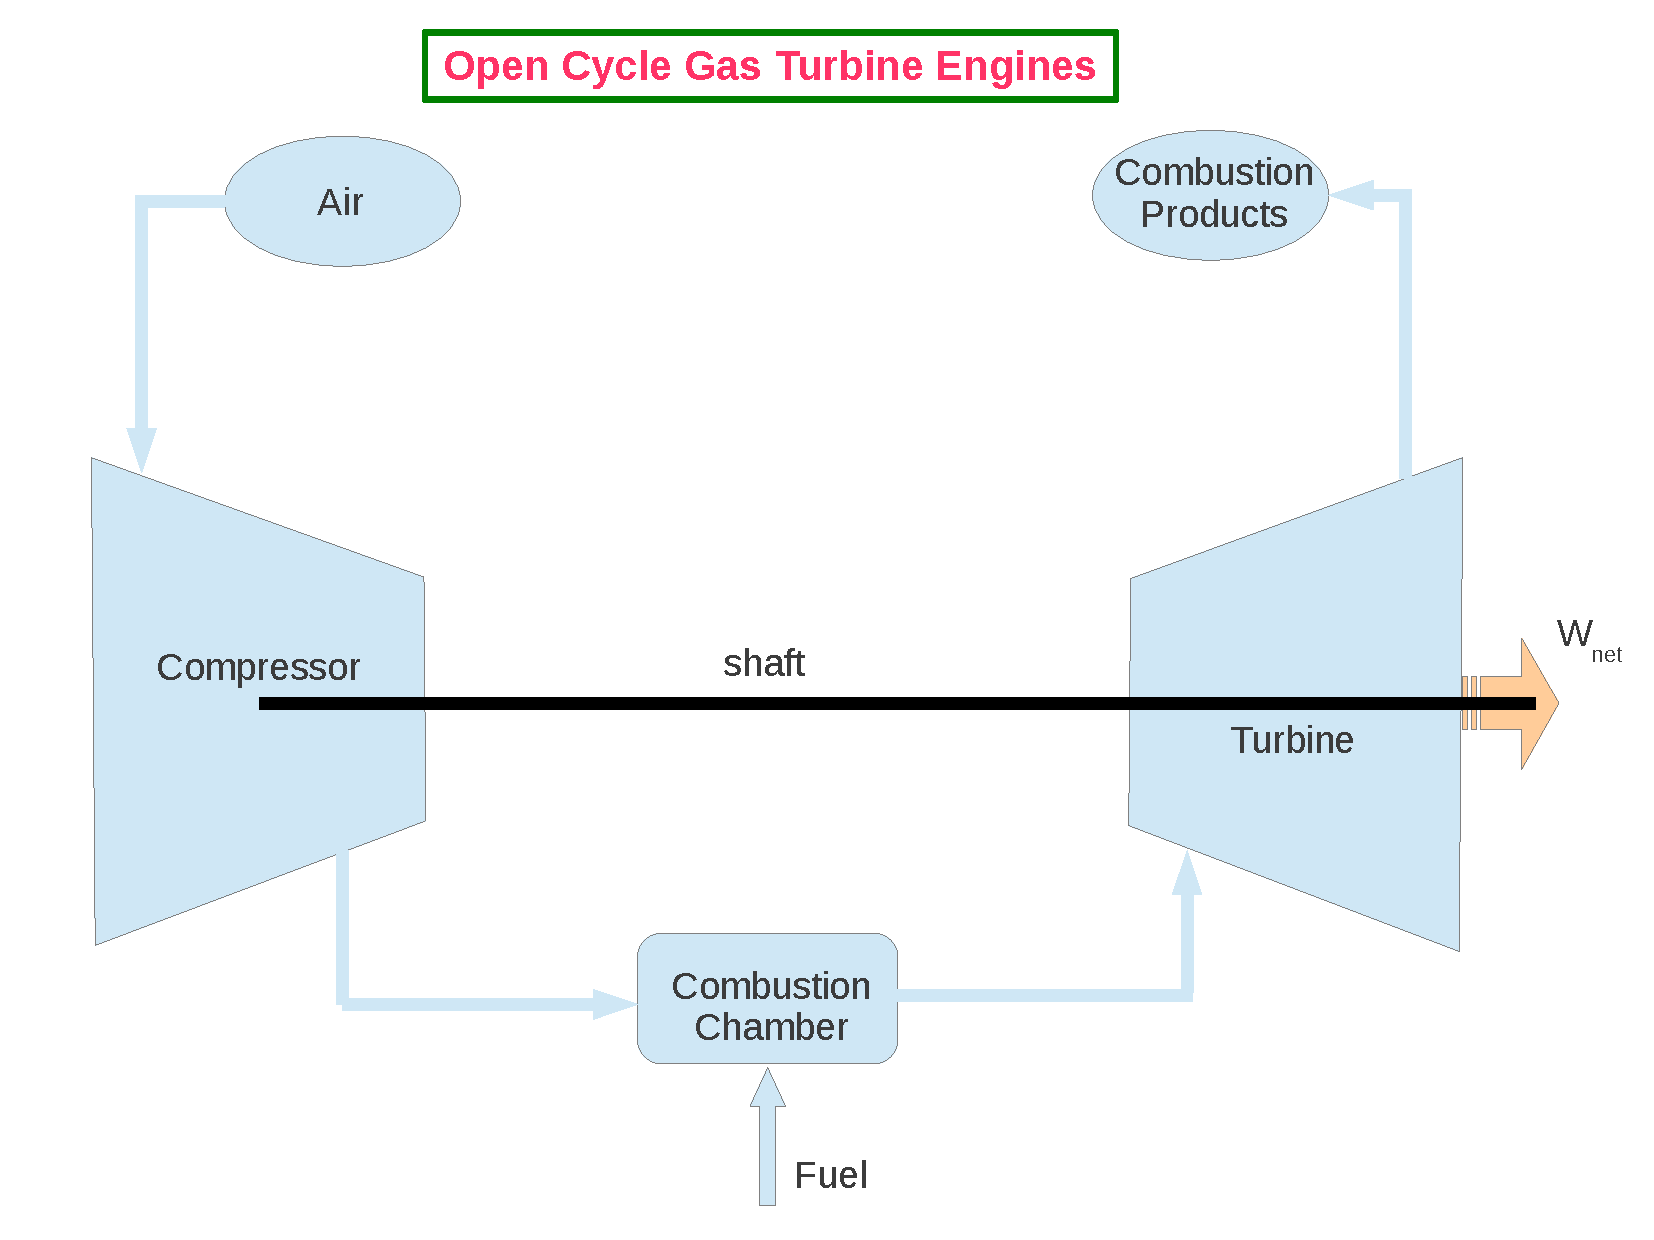
\includegraphics[width=5.8cm,clip]{./Pics/Open_Gas_Turbine_Engines}
         \end{center}
       \end{figure}} 
       \begin{enumerate}\setcounter{enumi}{7} \scriptsize
          \item<8-> In order to compare ideal and actual/real efficiencies, we introduce the relative efficiency:
             \visible<8->{\begin{equation}
                \textcolor{blue}{\eta_{\text{relative}}=\displaystyle\frac{\text{Actual Thermal Efficiency}}{\text{Air-Standard Efficiency}}}
             \end{equation}}
       \end{enumerate}
     \end{column}   
  \end{columns}  
\end{frame}


%%%
%%% SECTION
%%%
\section{Internal Combustion Engines}

%%%===            ===%%%
%%%=== SUBSECTION ===%%%
%%%===            ===%%%
\subsection{Reciprocating Engines}

%%%
%%% Slide
%%%
\begin{frame}
 \frametitle{Nomenclature}
 \begin{columns}
  \begin{column}[c]{0.5\linewidth}
   \begin{enumerate}[(1)]\scriptsize
    \item<1-> Components:
      \begin{enumerate}[(a)]\scriptsize
        \item<1-> \blue{Bottom Dead Center (BDC)}: position of the piston in which the volume becomes \red{maximum};
        \item<1-> \blue{Top Dead Center (TDC)}: position of the piston in which the volume becomes \red{minimum} (i.e., \underline{clearance volume});
        \item<1-> \blue{Bore}: diameter of the piston;
        \item<1-> The \blue{Intake Valve} is responsible to control the inflow of the air-fuel solution into the cylinder;
        \item<1-> The \blue{Exhaust Valve} lets the combustion gases leave the cylinder;
      \end{enumerate} 
    \item<2-> \blue{Stroke}: the largest distance that the piston can travel: $X_{\text{TDC}}-X_{\text{BDC}}$;
    \item<2-> \blue{Displacement Volume}: volume of the cylinder limited by $X_{\text{TDC}}$ and $X_{\text{BDC}}$
    \item<3-> \blue{Compression Ratio}: 
        \begin{equation}
           r = \frc{V_{\text{max}}}{V_{\text{min}}} = \frc{V_{\text{BDC}}}{V_{\text{TDC}}}
        \end{equation}
   \end{enumerate}
  \end{column}
  \begin{column}[c]{0.5\linewidth}
   \begin{figure}%
    \begin{center}
     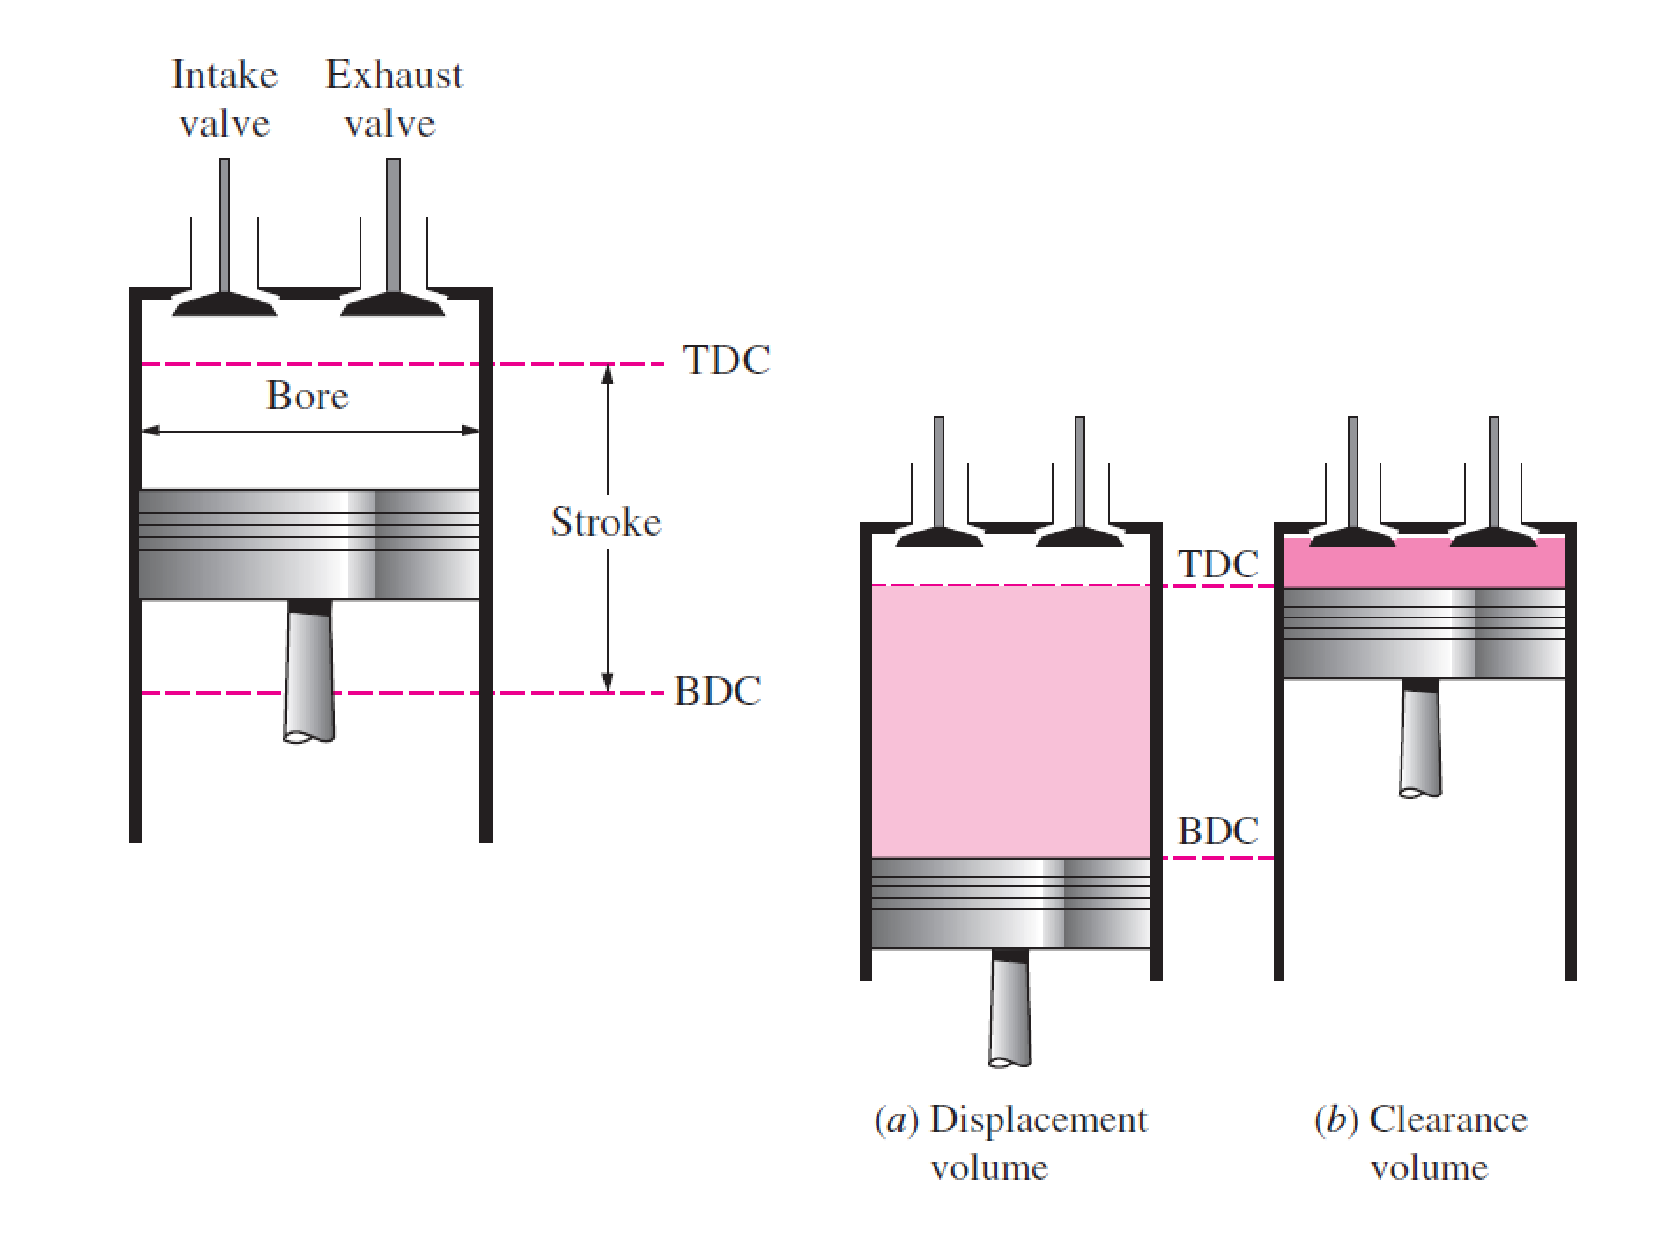
\includegraphics[width=6.2cm,clip]{./Pics/GasCycle_ReciprocatingEngine}
    \end{center}
   \end{figure} 
  \end{column}  
 \end{columns}
\begin{center}\scriptsize
\visible<1->{\red{Visualisation of reciprocating engines: \href{https://www.youtube.com/watch?v=LCGE5NbeOiw}{https://www.youtube.com/watch?v=LCGE5NbeOiw}}}\end{center}

\end{frame}

%%%
%%% Slide
%%%
\begin{frame}
 \frametitle{Nomenclature}
 \begin{columns}
  \begin{column}[c]{0.5\linewidth}
   \begin{enumerate}[(1)]\setcounter{enumi}{4} \scriptsize
     \item<1-> The \blue{Mean Effective Pressure (MEP)} of the cycle is a fictitious pressure that, if it acted on the piston during the entire power stroke, would {\it produce the same amount of net work as that produced during the actual cycle}:
        \visible<1->{\begin{eqnarray}
          && W_{\text{net}} = MEP \times \text{Piston area} \times \text{Stroke} \nonumber \\
          && MEP= \frc{W_{\text{net}}}{V_{\text{max}}-V_{\text{min}}}
        \end{eqnarray}} 
     \item<2-> MEP is used as a parameter to compare performances of reciprocating engines of equal size:  \blue{Larger MEP $\Longrightarrow$ larger $W_{\text{net}}$}. 
   \end{enumerate}
  \end{column}
  \begin{column}[c]{0.5\linewidth}
   \begin{figure}%
    \begin{center}
     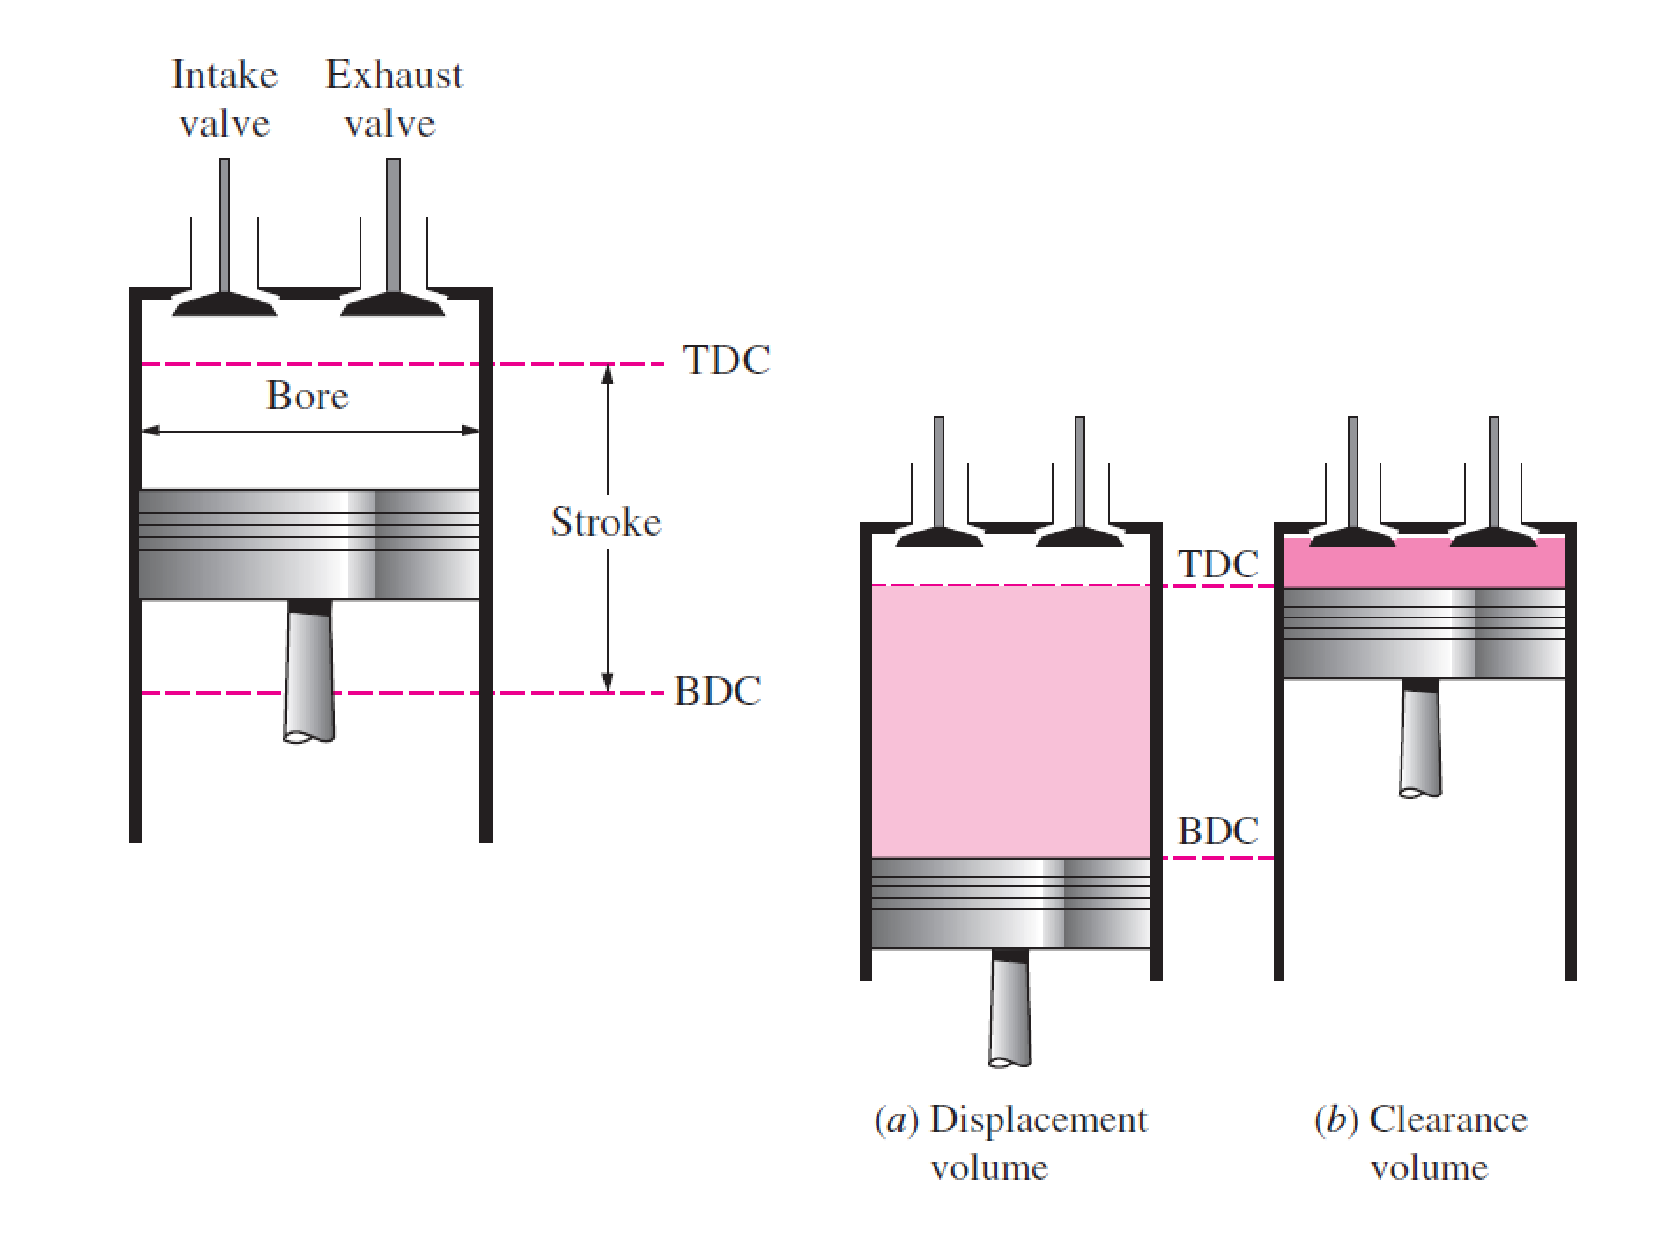
\includegraphics[width=6.2cm,clip]{./Pics/GasCycle_ReciprocatingEngine}
    \end{center}
   \end{figure} 
  \end{column}  
 \end{columns}
\end{frame}

%%%
%%% Slide
%%%
\begin{frame}
 \frametitle{Classification of Reciprocating Engines}
  \begin{columns}
   \begin{column}[c]{0.45\linewidth}\scriptsize
   
     \begin{enumerate}\scriptsize
      \item <2-> \blue{Spark Ignition (SI) Engines}: the combustion of the air–-fuel mixture is initiated by a spark plug (the mixture is at  \red{flash point} conditions);
       \begin{enumerate}\scriptsize
        %\item <4-> Fuel--air solution is compressed to $T<T_{\text{autoignition}}^{\text{fuel}}$ and combustion is initialised by a (electric) spark;
        \item <4-> Four stroke cycle: suction, compression, expansion (also called power or working) and exhaust;
        \item <5-> Two stroke cycle: compression and expansion;
       \end{enumerate}
      \item <3-> \blue{Compression Ignition (CI) Engines}: the air–-fuel mixture is self-ignited as a result of compressing the mixture above its self-ignition temperature.
       \begin{enumerate}\scriptsize
          \item <6-> \underline{Diesel cycle} is the ideal cycle for CI reciprocating engines;
          \item <7-> Strokes of the cycle: suction, compression, expansion and exhaust.
       \end{enumerate}
     \end{enumerate}
   \end{column}
   \begin{column}[c]{0.55\linewidth}
    \begin{figure}%
     \begin{center}
      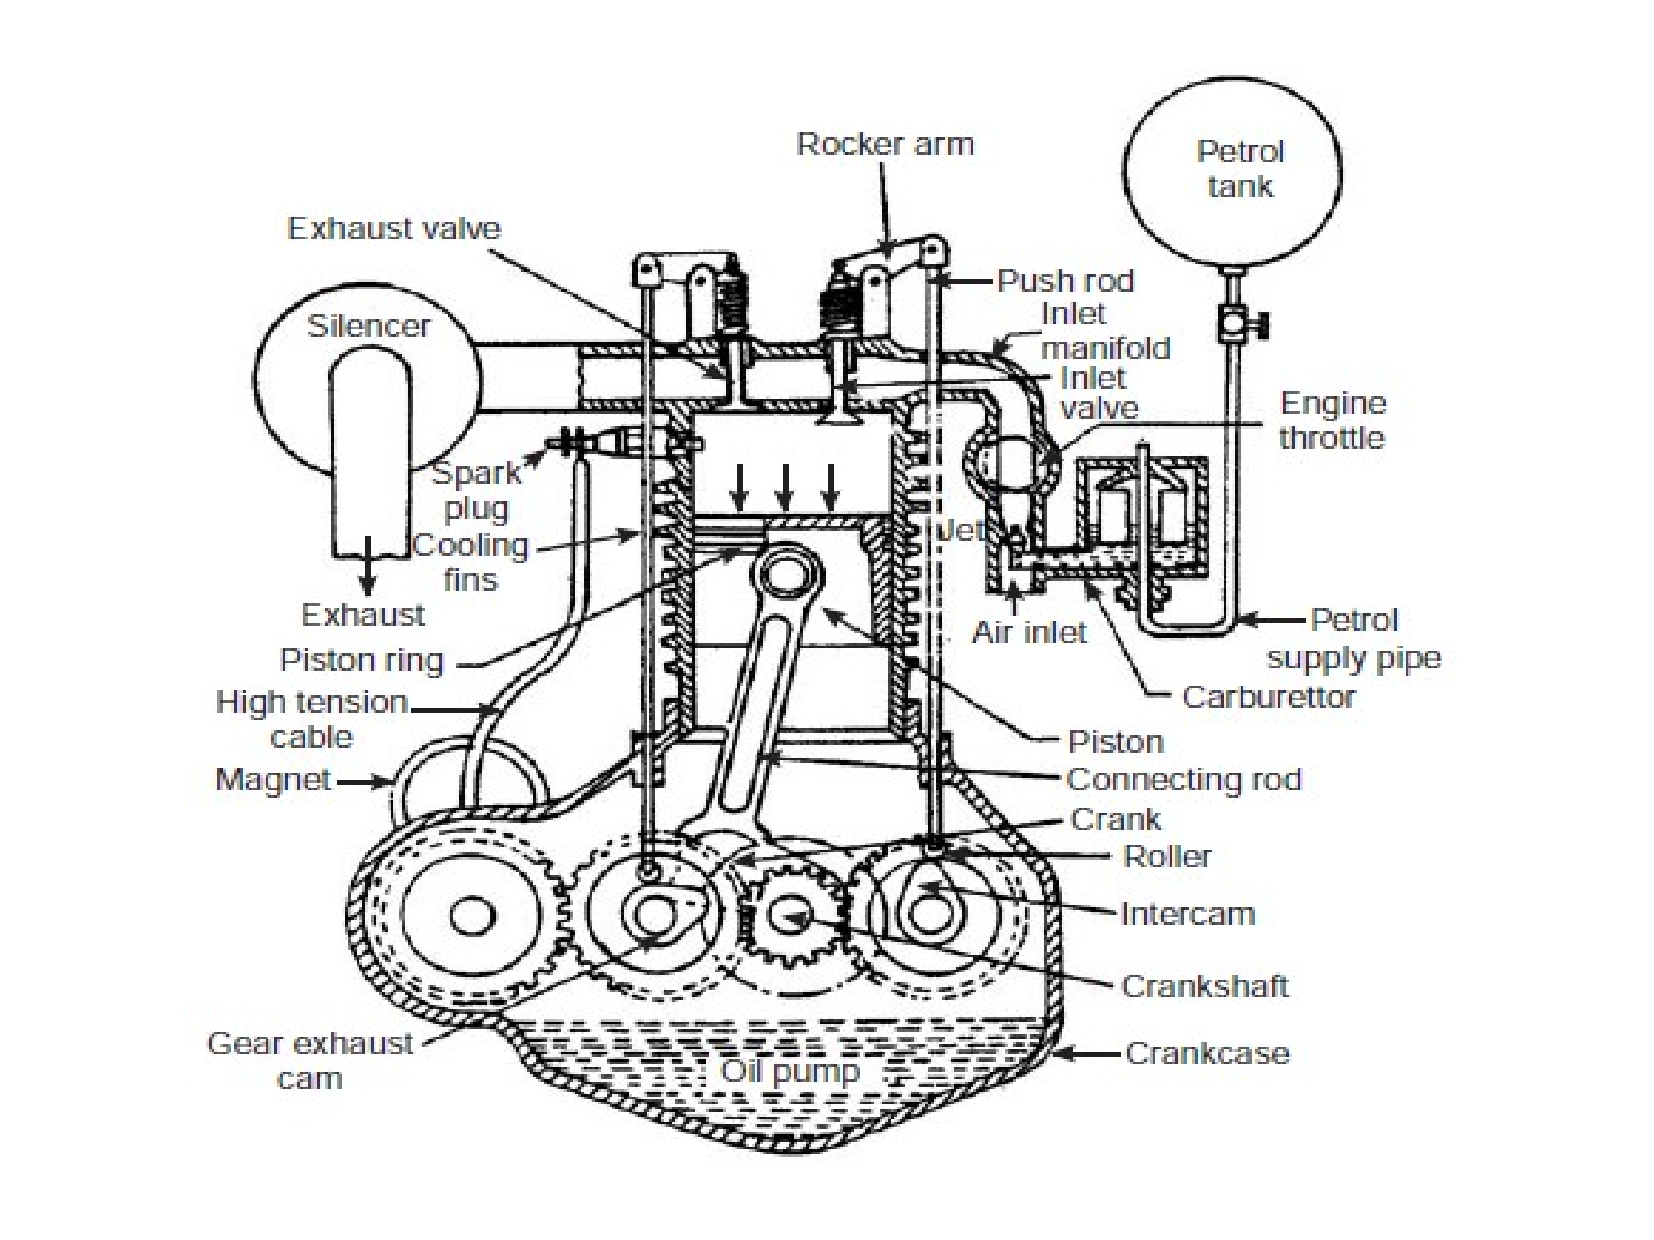
\includegraphics[width=7.5cm,clip]{./Pics/InternalCombustion_4Strokes}
      \scriptsize\caption{\scriptsize Air-cooled four-stroke petrol engine.}
     \end{center}
    \end{figure}  
   \end{column}  
  \end{columns}
\end{frame}


%%%===            ===%%%
%%%=== SUBSECTION ===%%%
%%%===            ===%%%
\subsection{Ideal Carnot Cycle}
%%%
%%% Slide
%%%
\begin{frame}
 \frametitle{Carnot Cycle}
 \begin{columns}
  \begin{column}[c]{0.45\linewidth}
   \begin{enumerate}[(1)] \scriptsize
     \item<1-> \blue{Carnot cycle} has the highest possible efficiency and, similarly from previous lectures, consists of four stages:
     \begin{itemize}\scriptsize
       \item<1-> {\bf 1-2}: Isothermal expansion; 
       \item<1-> {\bf 2-3}: Adiabatic expansion;
       \item<1-> {\bf 3-4}: Isothermal compression;
       \item<1-> {\bf 4-1}: Adiabatic compression.
     \end{itemize}\scriptsize
     \item <2-> The efficiency of the cycle is then given by
       \begin{eqnarray}
        \textcolor{blue}{\eta_{\text{Carnot}}} &=& \displaystyle\frac{\text{work done}}{\text{heat supplied}} \nonumber\\
                         &=& \displaystyle\frac{\text{heat supplied}-\text{heat rejected}}{\text{heat supplied}} \nonumber \\
                         &=& \displaystyle\frac{Q_{s}-Q_{r}}{Q_{s}} = \displaystyle\frac{T_{1}-T_{2}}{T_{1}} \nonumber  \\
                         &=&  \blue{1 - \frc{T_{2}}{T_{1}}}
       \end{eqnarray}
     \item<3-> The efficiency of the cycle can be readily enhanced if the $T_{2}$ decreases. And in the limit,
        \begin{displaymath}
           \lim_{T_{2} \to 0}\eta_{\text{Carnot}} = 1
        \end{displaymath}
   \end{enumerate}
  \end{column}
  \begin{column}[c]{0.55\linewidth}
   \begin{enumerate}[(1)]\setcounter{enumi}{3} \scriptsize
     \item<4-> We can not produce a system that can move
     \begin{enumerate}[(a)] \scriptsize
        \item<4-> very slow in the \blue{isothermal expansion} ($\lq$forward stroke') and;
        \item<4-> very fast during the remainder of the adiabatic expansion. 
     \end{enumerate}
     \item<5-> The cycle would become \red{unfeasible}.
   \end{enumerate} 
   \begin{figure}%
    \begin{center}
     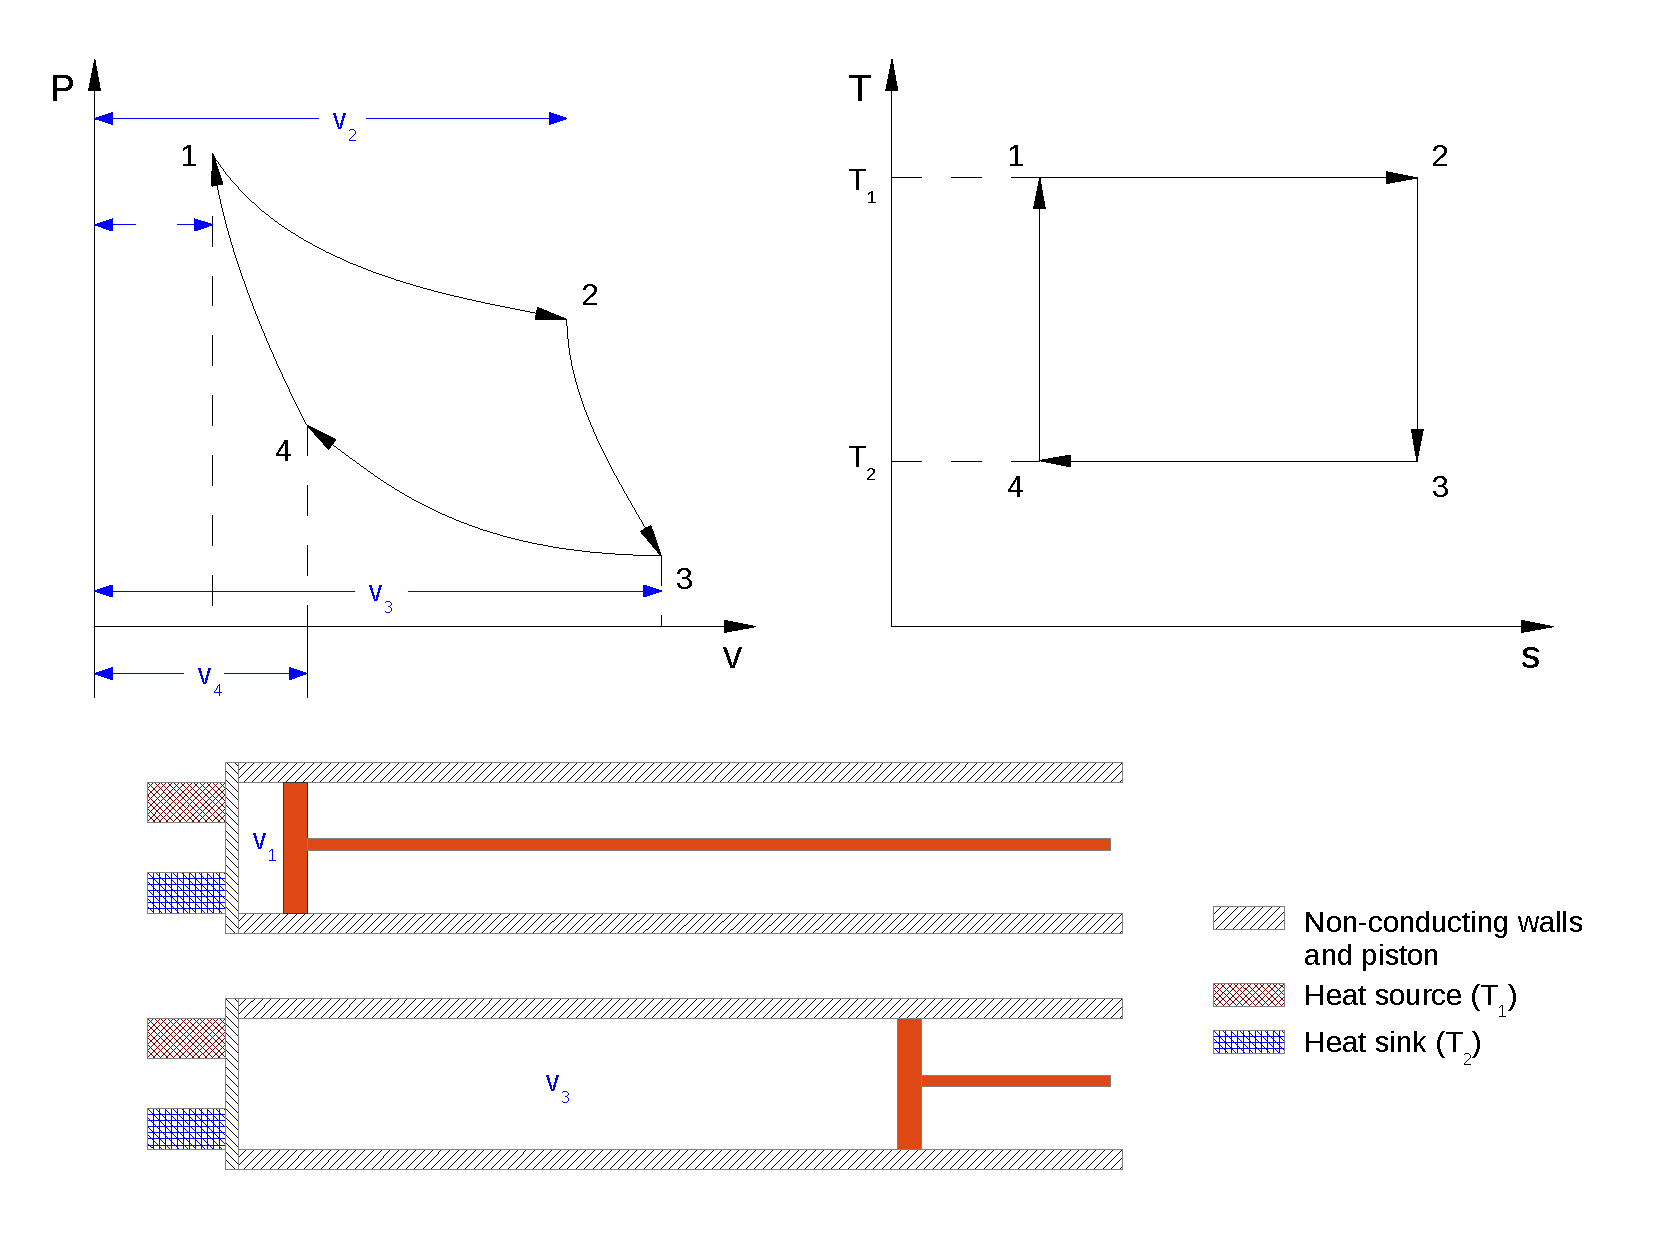
\includegraphics[width=6.5cm,clip]{./Pics/Carnot_Reciprocating}
    \end{center}
   \end{figure} 
  \end{column}  
 \end{columns} 
\end{frame}

%%%
%%% Slide
%%%
\begin{frame}
 \frametitle{Example 1: Carnot Cycle (Problem 1)}
     In a Carnot cycle, the maximum pressure and temperature are limited to 18 bar and 410$^{\circ}$C. The ratio of isentropic compression and isothermal expansion are 6 and 1.5, respectively. Assuming the volume of the air at the beginning of isothermal expansion is 0.18 m$^{3}$, determine:
       \begin{enumerate}[(a)]
          \item Temperature and pressures at all stages of the cycle; 
          \item Change in entropy $\left(\text{in kJ.K}^{-1}\right)$ during isothermal expansion. Entropy variation for ideal gases is given by
             \begin{displaymath}
                \frc{\Delta S}{R} = \int\limits_{T_{0}}^{T}\frc{C_{p}^{ig}}{R}\frc{d T}{T}-\ln\frc{P}{P_{0}};
             \end{displaymath}
          \item Mean thermal efficiency of the cycle; 
          \item Mean effective pressure (MEP) of the cycle and;
          \item Theoretical power if there are 210 working cycles per minute.
       \end{enumerate}
\end{frame}



%%%===            ===%%%
%%%=== SUBSECTION ===%%%
%%%===            ===%%%
\subsection{Otto Cycle (Constant Volume)}

%%%
%%% Slide
%%%
\begin{frame}
 \frametitle{Four-Strokes Internal Combustion Engines}
  \begin{columns}
   \begin{column}[c]{0.4\linewidth}
    \begin{enumerate}[(1)]\scriptsize
     \item<1-> Fuel--air solution is compressed to a \blue{temperature just below the auto--ignition temperature of the fuel} and combustion is initialised by an electrical spark;
     \item<2-> \blue{Suction stroke (SS):} also called \blue{intake stroke}. The mixture is injected through the intake valve (IV). The exhaust valve (EV) remains closed during this stage;
     \item<3-> \red{Compression stroke (CS):} whereas IV and EV remain closed, pressure and temperature of the solution rise. Near the end of CS, the fuel is ignited by an electric spark, leading to the combustion of the fuel (consumption of carbon);
     \item<4-> \blue{Expansion stroke (WS):} also called \blue{power} or \blue{working} stroke. IV and EV remain closed and near the completion of the this stroke, the \blue{EV} is opened and the pressure in the cylinder push most of the gases out of the cylinder;
    \end{enumerate}
   \end{column}
   \begin{column}[c]{0.6\linewidth}
    \begin{figure}%
     \begin{center}
      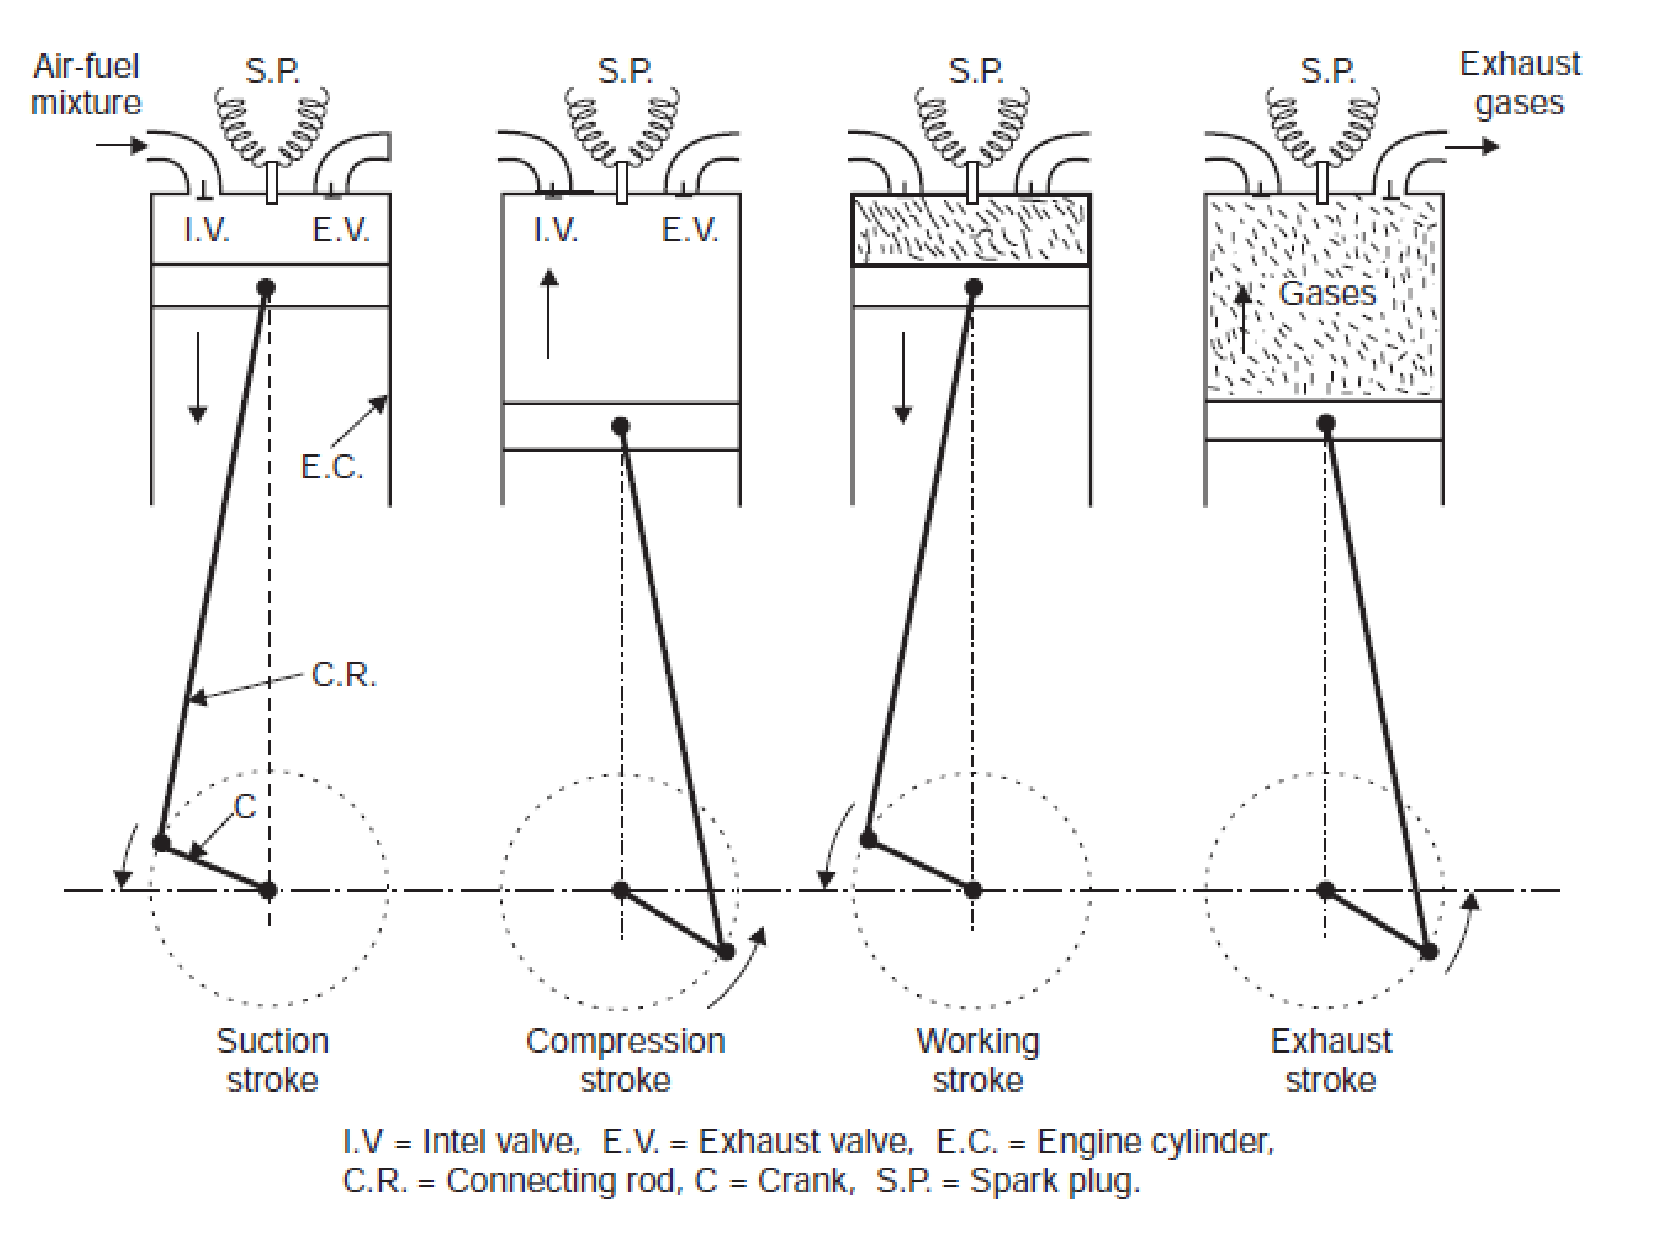
\includegraphics[width=6.5cm,clip]{./Pics/InternalCombustion_4Strokes_Otto}
      %\caption{Air-cooled four-stroke petrol engine.}
     \end{center}
    \end{figure}  
    \begin{enumerate}[(1)]\setcounter{enumi}{4}\scriptsize
      \item<5-> \red{Exhaust stroke (ES):} all remaining gases are removed from the cylinder. While the IV remains closed the \blue{piston returns to the top dead centre (TDC)}.
    \end{enumerate}
   \end{column}  
  \end{columns}
\vspace{0.cm}\begin{center}\scriptsize
\visible<1->{\textcolor{red}{Visualisation of the 4-strokes engine: \href{http://www.animatedengines.com/otto.html}{http://www.animatedengines.com/otto.html} }}\end{center}
\end{frame}


%%%
%%% Slide
%%%
\begin{frame}
 \frametitle{Two-Strokes Internal Combustion Engines}
  \begin{columns}
   \begin{column}[c]{0.5\linewidth}
    \begin{enumerate}[(1)]\scriptsize
     \item<1-> In this class of engines, \blue{both suction and exhaust strokes are eliminated}, and valves are replaced by ports;
     \item<2-> Exhaust gases are driven out of the cylinder by the fresh intake of mixing fuel + air \blue{at the end of the expansion stroke};
     \item<3-> Piston moves upwards compressing the fuel mixture (\textcolor{blue}{L}) previously supplied by \textcolor{blue}{V}. Ignition occurs in the end of the stroke (max compression);
     \item<4-> Piston moves downwards due to the gases expansion and near the end of the stroke; 
     \item<5-> Piston uncovers the \textcolor{blue}{exhausted port (EP)} and the gases are allowed to escape. The \textcolor{blue}{transfer port (TP)} is uncovered and the fresh fuel enters the cylinder driving away the remaining exhausted gases;
    \end{enumerate}
   \end{column}
   \begin{column}[c]{0.5\linewidth}
    \begin{figure}%
     \begin{center}
      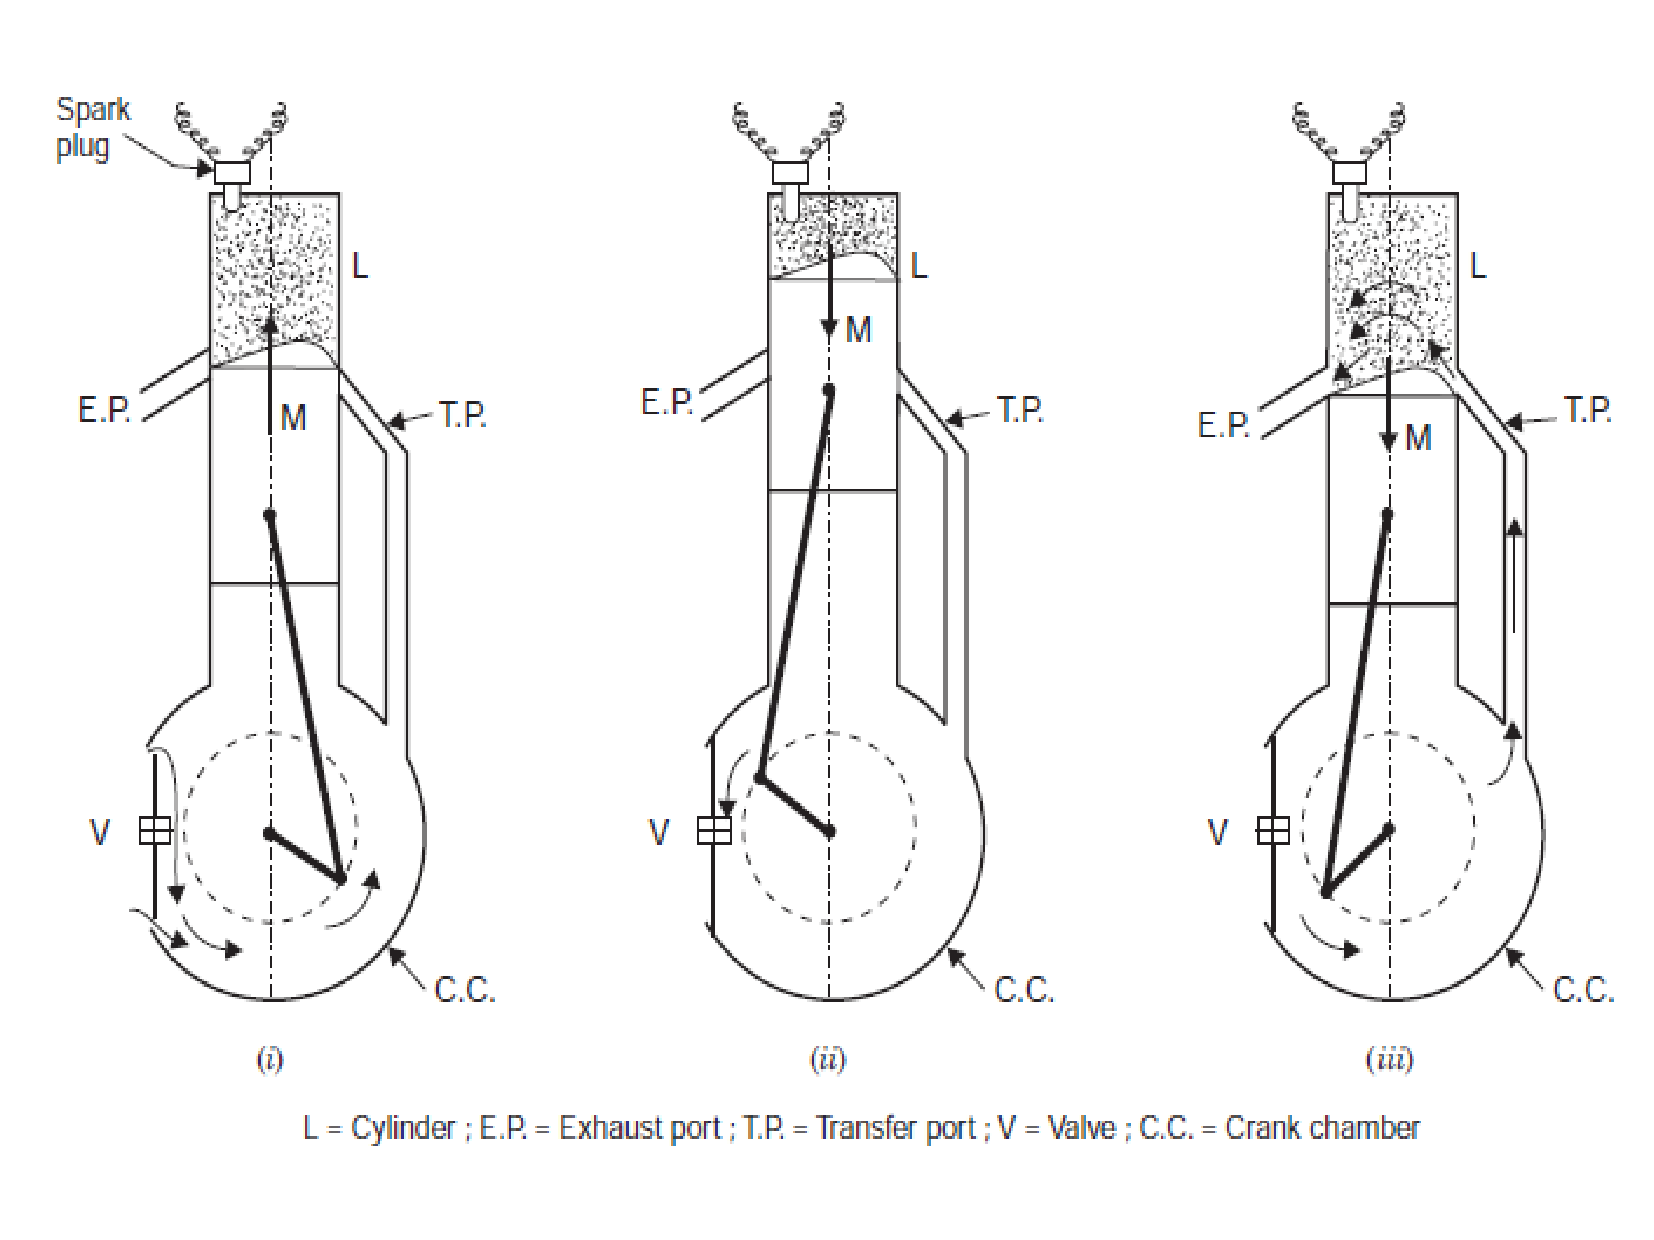
\includegraphics[width=6.cm,clip]{./Pics/InternalCombustion_2Strokes_Otto}
      %\caption{Air-cooled four-stroke petrol engine.}
     \end{center}
    \end{figure}  
   \end{column}  
  \end{columns}
\vspace{0.5cm}\begin{center}\scriptsize
\visible<1->{\textcolor{red}{Visualisation of the 2-strokes engine: \href{http://www.animatedengines.com/twostroke.html}{http://www.animatedengines.com/twostroke.html} }}\end{center}
\end{frame}


%%%
%%% Slide
%%%
\begin{frame}
 \frametitle{Actual and Ideal Otto Cycles}\scriptsize
    \red{Air-standard Otto cycle} is an ideal cycle that assumes the heat addition occurs instantaneously while the piston is at TDC.
    \begin{figure}%
     \begin{center}
      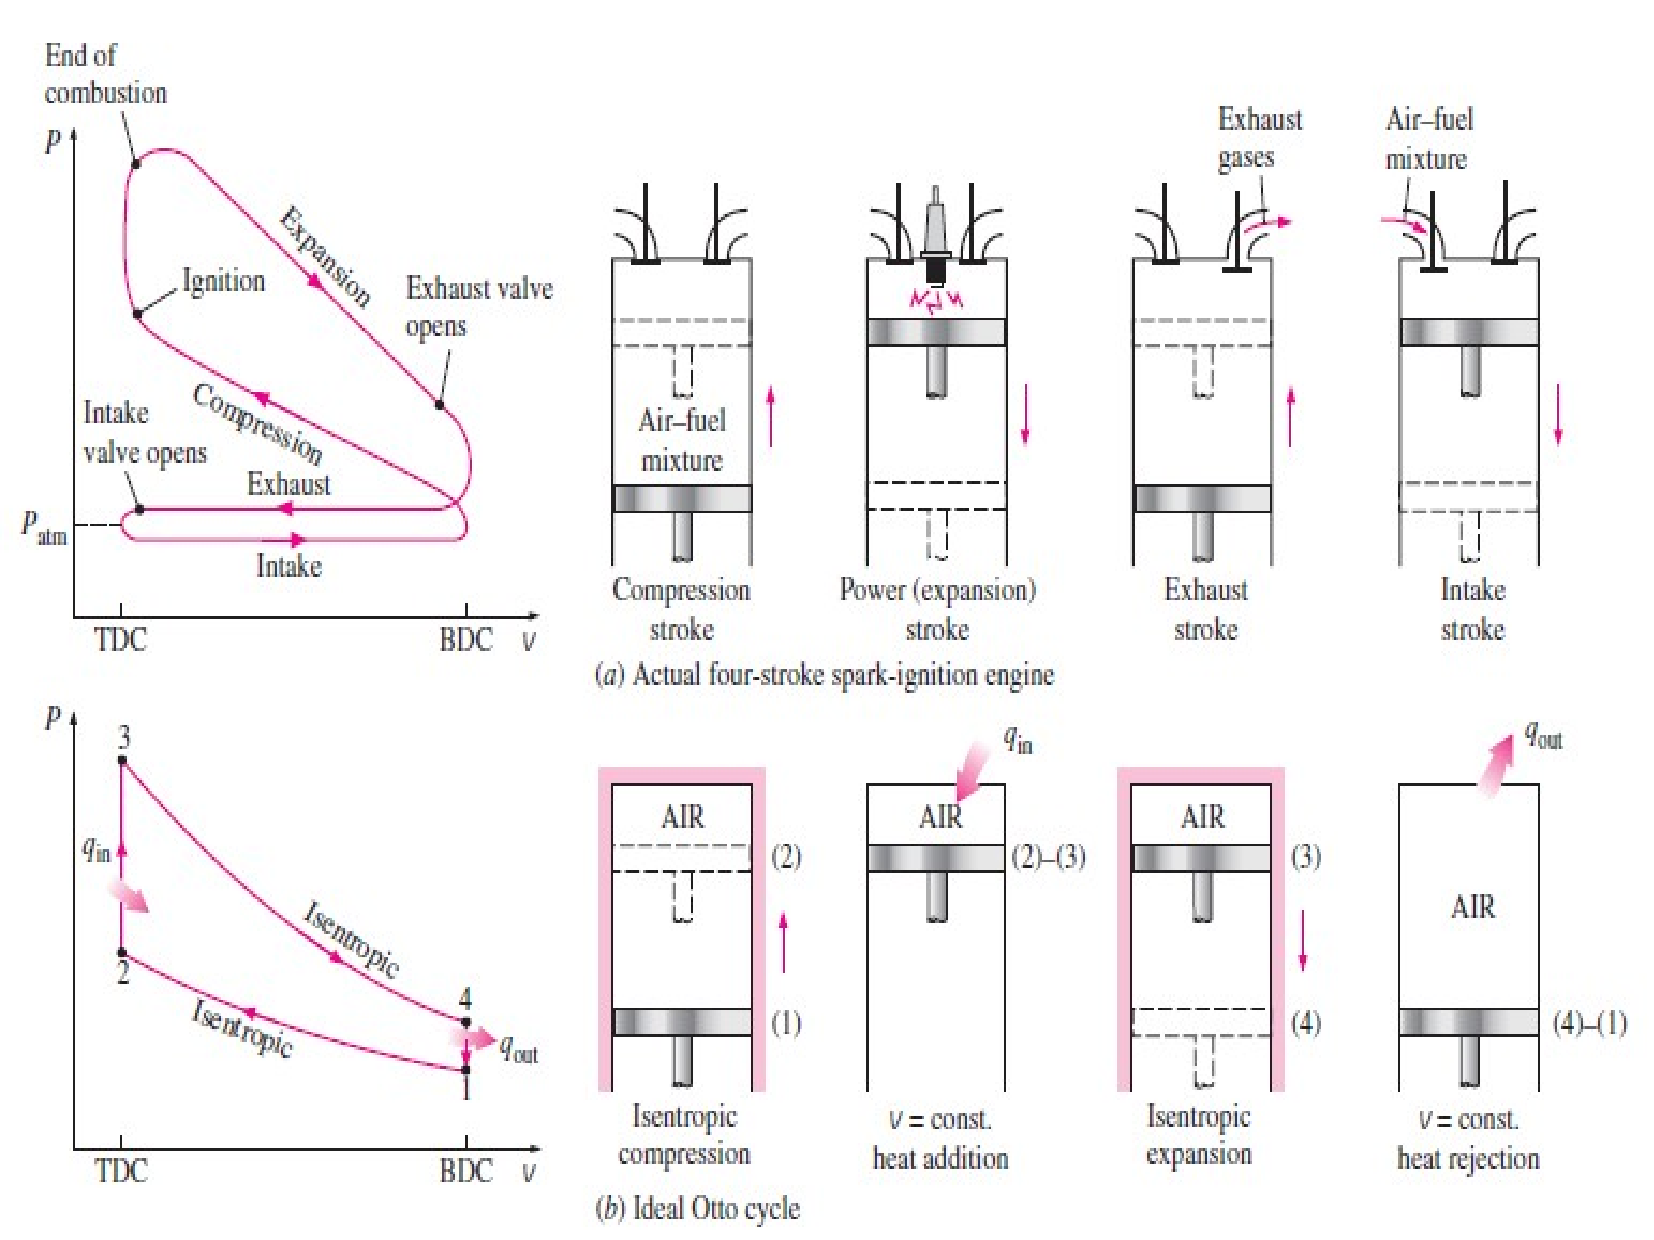
\includegraphics[width=9.cm,clip]{./Pics/InternalCombustion_IdealOttoCycle}
     %\caption{Actual and ideal cycles in SI engines and their associated Pv diagrams.}
     \end{center}
    \end{figure} 
\end{frame}

%%%
%%% Slide
%%%
\begin{frame}
 \frametitle{Ideal Otto Cycles}
  \begin{columns}
   \begin{column}[c]{0.6\linewidth}
    \begin{enumerate}[(1)]\scriptsize
      \item<1-> Four strokes:
      \begin{enumerate}[(a)]\scriptsize
         \item<1-> {\bf 1-2}: Isentropic compression of air;
         \item<1-> {\bf 2-3}: Addition of heat, $Q_{in}$, at \blue{constant volume};
         \item<1-> {\bf 3-4}: Isentropic expansion;
         \item<1-> {\bf 4-1}: Rejection of heat, $Q_{out}$, at \blue{constant volume}.
      \end{enumerate}
      \item<2-> Since ideal Otto cycle is composed of \blue{internally reversible processes}, areas on the {\it Ts} and {\it Pv} diagrams can be interpreted as \blue{heat and work}. Therefore, the energy balance for 1 kg of air is:
      \item<3-> Heat supplied at constant volume:
         \visible<3->{\begin{displaymath}
            Q_{in} = C_{v}\left(T_{3}-T_{2}\right)
         \end{displaymath}}
      \item<4-> Heat rejected at constant volume:
         \visible<3->{\begin{displaymath}
            Q_{out} = C_{v}\left(T_{4}-T_{1}\right)
         \end{displaymath}}
      \item<5-> Net Work = Heat supplied - Heat rejected
         \visible<3->{\begin{displaymath}
            W_{\text{net}}=C_{v}\left(T_{3}-T_{2}\right) - C_{v}\left(T_{4}-T_{1}\right)
         \end{displaymath}} 
    \end{enumerate}
   \end{column}
   \begin{column}[c]{0.4\linewidth}
    \begin{figure}%
     \begin{center}
      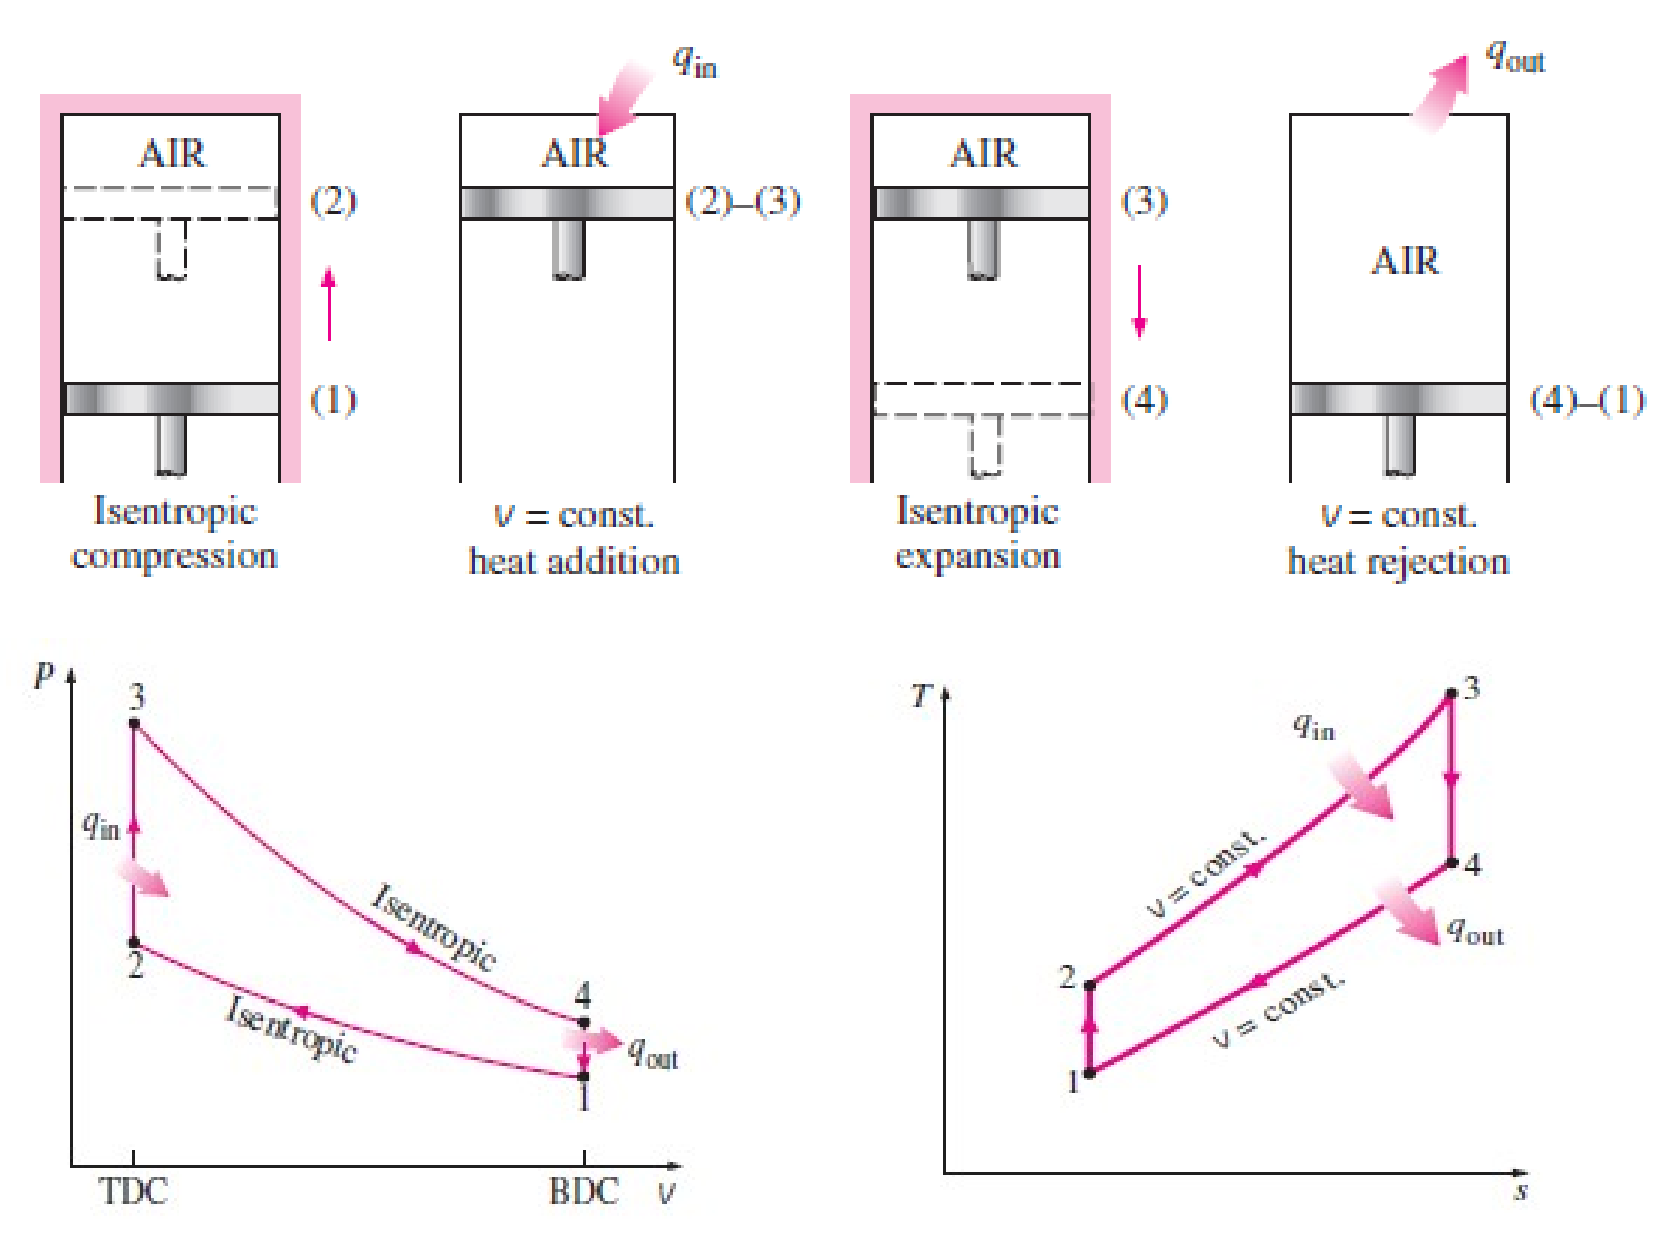
\includegraphics[width=5.cm,clip]{./Pics/InternalCombustion_IdealOttoCycle2}
     \end{center}
    \end{figure}  
    \begin{enumerate}[(1)]\setcounter{enumi}{5}\scriptsize
      \item<6-> Efficiency:
         \visible<3->{\begin{equation}
            \eta_{\text{Otto}} = \frc{W_{\text{net}}}{Q_{\text{in}}} = 1 - \frc{T_{4}-T_{1}}{T_{3}-T_{2}} \label{OttoEfficiency1}
         \end{equation}} 
    \end{enumerate}
   \end{column}  
  \end{columns}
\end{frame}

%%%
%%% Slide
%%%
\begin{frame}
 \frametitle{Ideal Otto Cycles}
  \begin{columns}
   \begin{column}[c]{0.6\linewidth}
    \begin{enumerate}[(1)]\setcounter{enumi}{6}\scriptsize
      \item<1-> Compression $\left(\text{r}_{c}\right)$ and expansion $\left(\text{r}_{e}\right)$ ratios:
         \visible<1->{\begin{displaymath}
            r_{c} =\frc{V_{1}}{V_{2}}=r \;\;\;\text{ and }\;\;\; r_{e} =\frc{V_{4}}{V_{3}}=r
         \end{displaymath}}
      \item<2-> \blue{1-2} and \blue{3-4} are \red{isentropic}, therefore
         \visible<2->{\begin{displaymath}
            \frc{T_{2}}{T_{1}}=\left(\frc{V_{1}}{V_{2}}\right)^{\gamma-1}=r^{\gamma-1}\;\;\;\text{ and }\;\;\;\frc{T_{3}}{T_{4}}=\left(\frc{V_{4}}{V_{3}}\right)^{\gamma-1}=r^{\gamma-1}
         \end{displaymath}
         where $\gamma = \frc{C_{p}}{C_{v}}$ is the specific heat ratio.}
      \item<3-> As V$_{2}$=V$_{3}$ and V$_{1}$=V$_{4}$, replacing T$_{2}$ and T$_{3}$ in Eqn.~\ref{OttoEfficiency1} for Otto efficiency as a function of the compression ratio:
         \visible<3->{\begin{equation}
            \eta_{\text{Otto}} = 1 - \frc{1}{r^{\gamma-1}}
         \end{equation}
         This expression is called the \blue{air-standard efficiency of the Otto cycle}.}
      \item<4-> With the \blue{pressure ratio} $\left(r_{p} = \frc{P_{3}}{P_{2}} = \frc{P_{4}}{P_{1}}\right)$, the \blue{MEP} is
    \end{enumerate}
   \end{column}
   \begin{column}[c]{0.4\linewidth}
    \begin{figure}%
     \begin{center}
      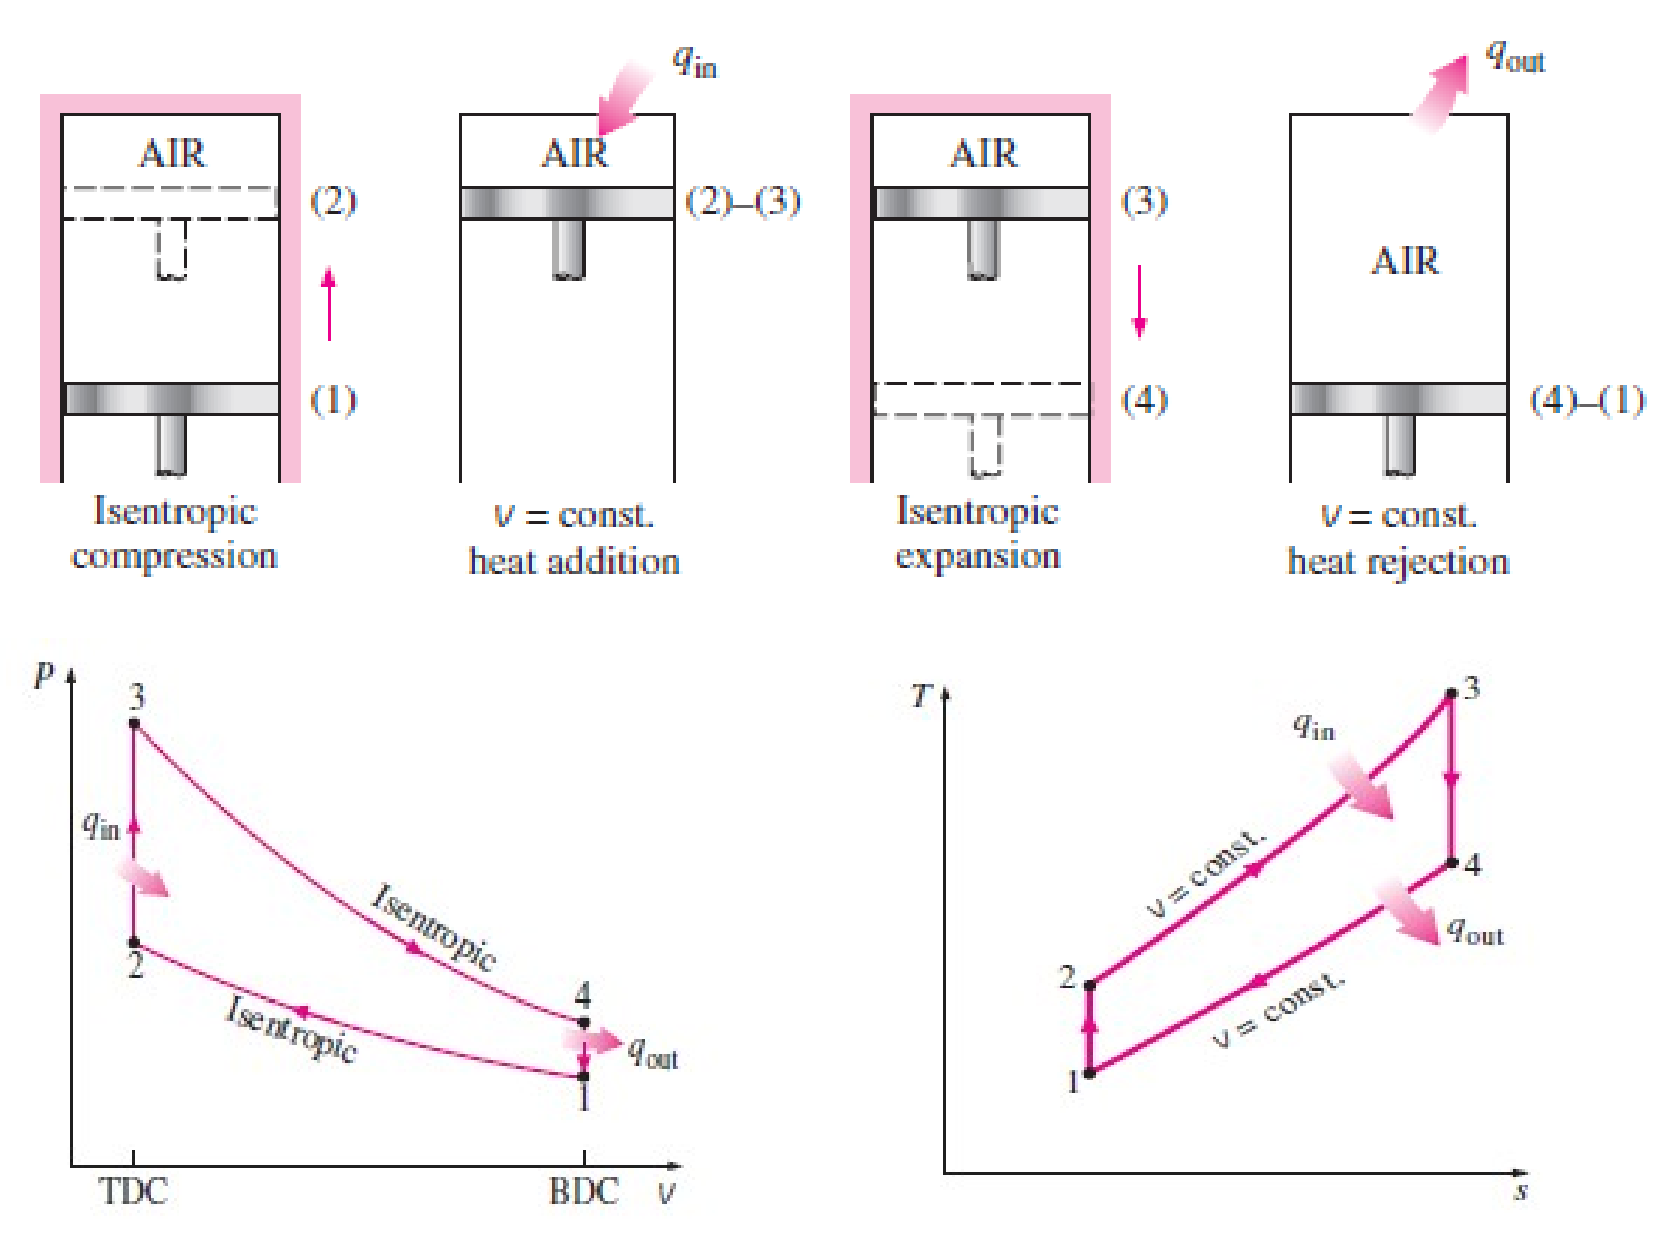
\includegraphics[width=5.cm,clip]{./Pics/InternalCombustion_IdealOttoCycle2}
     \end{center}
    \end{figure}  
    \visible<4->{\begin{equation}\scriptsize
       MEP = \frc{P_{1}r\left[\left(r^{\gamma-1} - 1\right)\left(r_{p}-1\right)\right]} {\left(\gamma-1\right)\left(r-1\right)}
    \end{equation}}
   \end{column}  
  \end{columns}
\end{frame}

%%%===            ===%%%
%%%=== SUBSECTION ===%%%
%%%===            ===%%%
\subsection{Diesel Cycle (Constant Pressure)}
%%%
%%% Slide
%%%
\begin{frame}
 \frametitle{Ideal Diesel Cycles}
  \begin{columns}
   \begin{column}[c]{0.6\linewidth}
    \begin{enumerate}[(1)]\scriptsize
     \item<1-> The Diesel cycle is the ideal cycle for \blue{compression-ignition} reciprocating engines;
     \item<2-> \blue{Only air is compressed} in the {\it compression stroke} -- eliminating the possibility of autoignition;
     \item<3-> Combustion starts on contact as the fuel is injected into the hot air -- \blue{$T>T^{\text{fuel}}_{\text{auto-ignition}}$};
     \item<4-> \underline{Spark plug and carburetor} are replaced by \underline{fuel injector};
     \item<5-> Diesel engines can be designed to operate at \blue{much higher compression ratios} -- typically 12$\leq$r$\leq$24.
     \item<6-> Fuel injection starts when the piston approaches \blue{TDC} and;
     \item<6-> Continues during the first part of the expansion stroke;
     \item<7-> Combustion process occurs over a longer interval and, therefore the \underline{cycle can be approximated} as a \red{constant-pressure heat-addition process};
     \item<8-> \red{this is the only difference between Otto and Diesel cycles}.
     \item<9-> Cycle:
        \begin{enumerate}[(a)]\scriptsize
          \item<10-> {\bf 1-2}: Isentropic compression $\left(\text{PV}^{\gamma}=\text{constant}\right)$;
          \item<10-> {\bf 2-3}: Heat addition at \underline{constant pressure};
          \item<10-> {\bf \red{3}}: \red{point of cut-off};
          \item<10-> {\bf 3-4}: Isentropic expansion;
          \item<10-> {\bf 4-1}: Heat rejection at \underline{constant volume};
        \end{enumerate}
    \end{enumerate}
   \end{column}
   \begin{column}[c]{0.4\linewidth}
    \begin{figure}%
     \begin{center}
      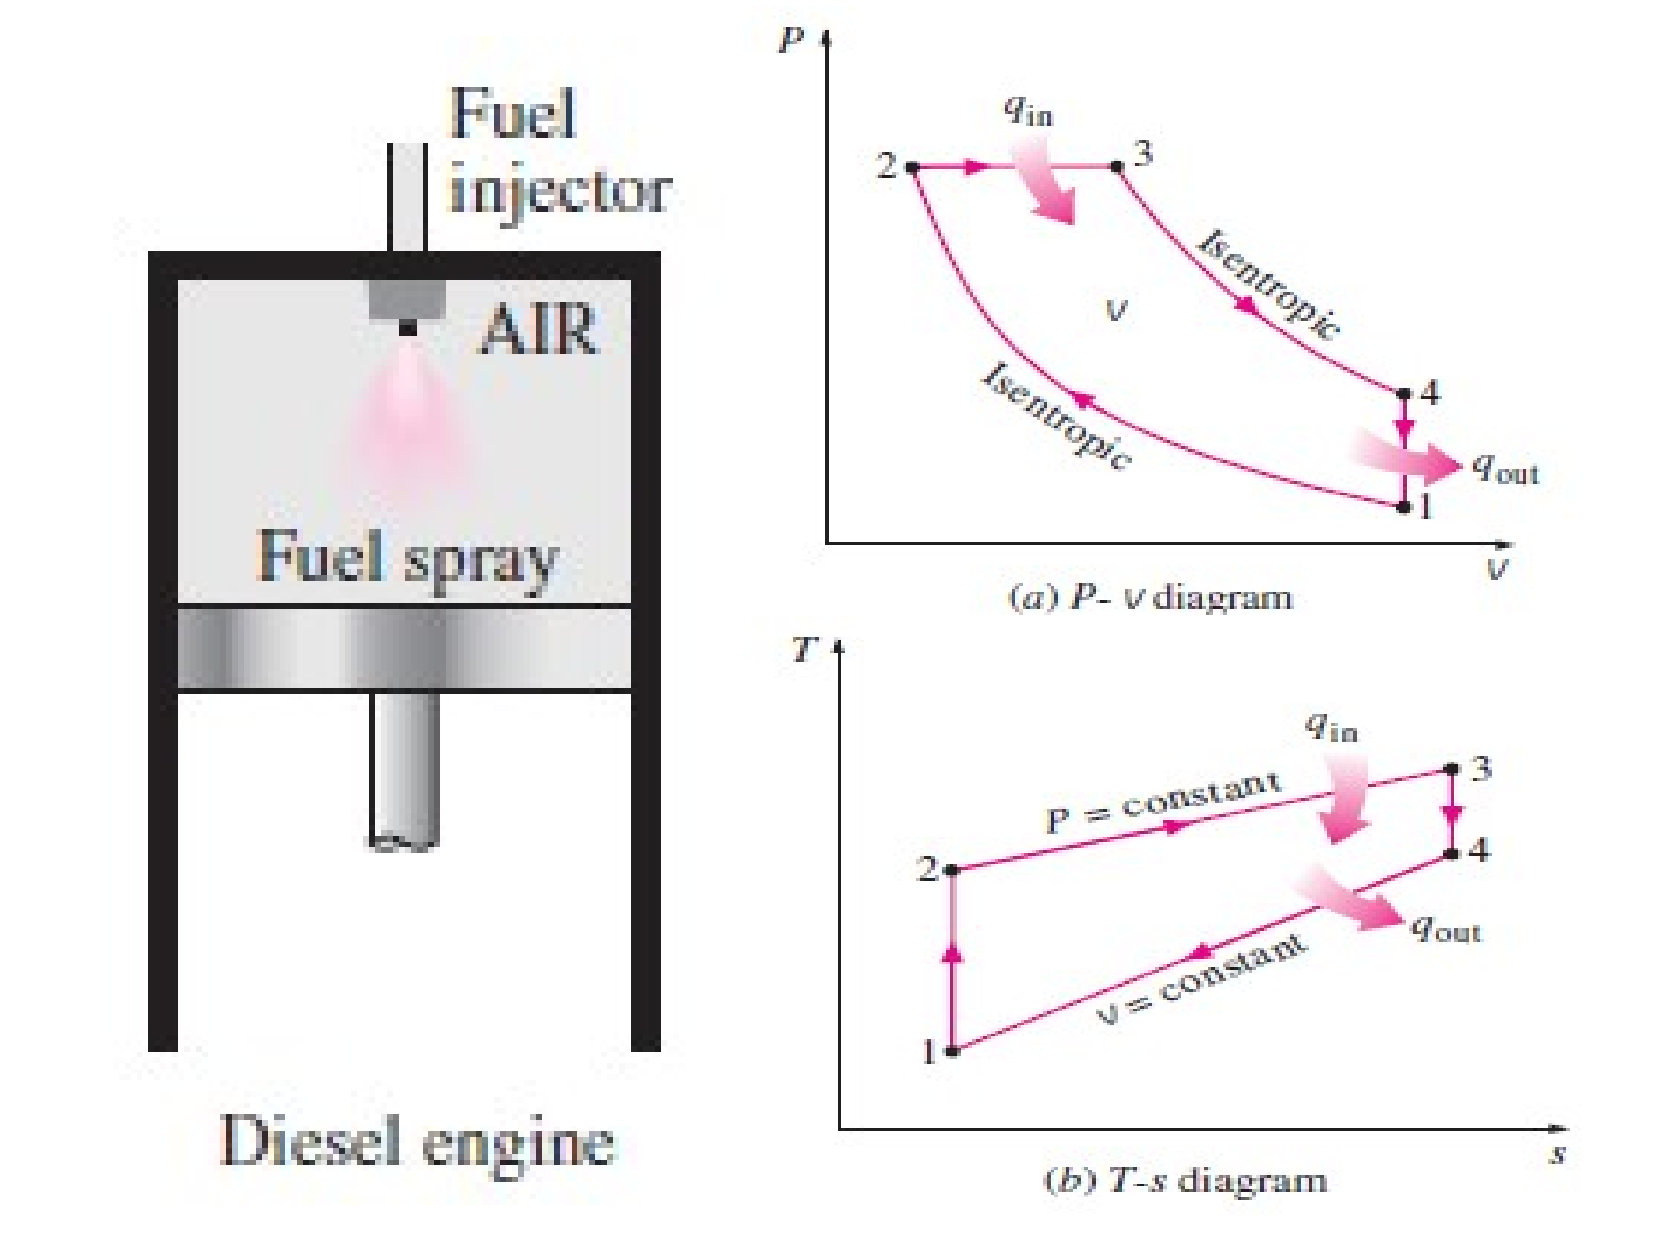
\includegraphics[width=5.cm,clip]{./Pics/InternalCombustion_IdealDieselCycle}
     \end{center}
    \end{figure}   
   \end{column}  
  \end{columns}
\end{frame}

%%%
%%% Slide 
%%%
\begin{frame}
 \frametitle{{\it Pv} and {\it Ts} Diagrams: Ideal Otto and Diesel Cycles}
    \begin{figure}%
     \begin{center}
      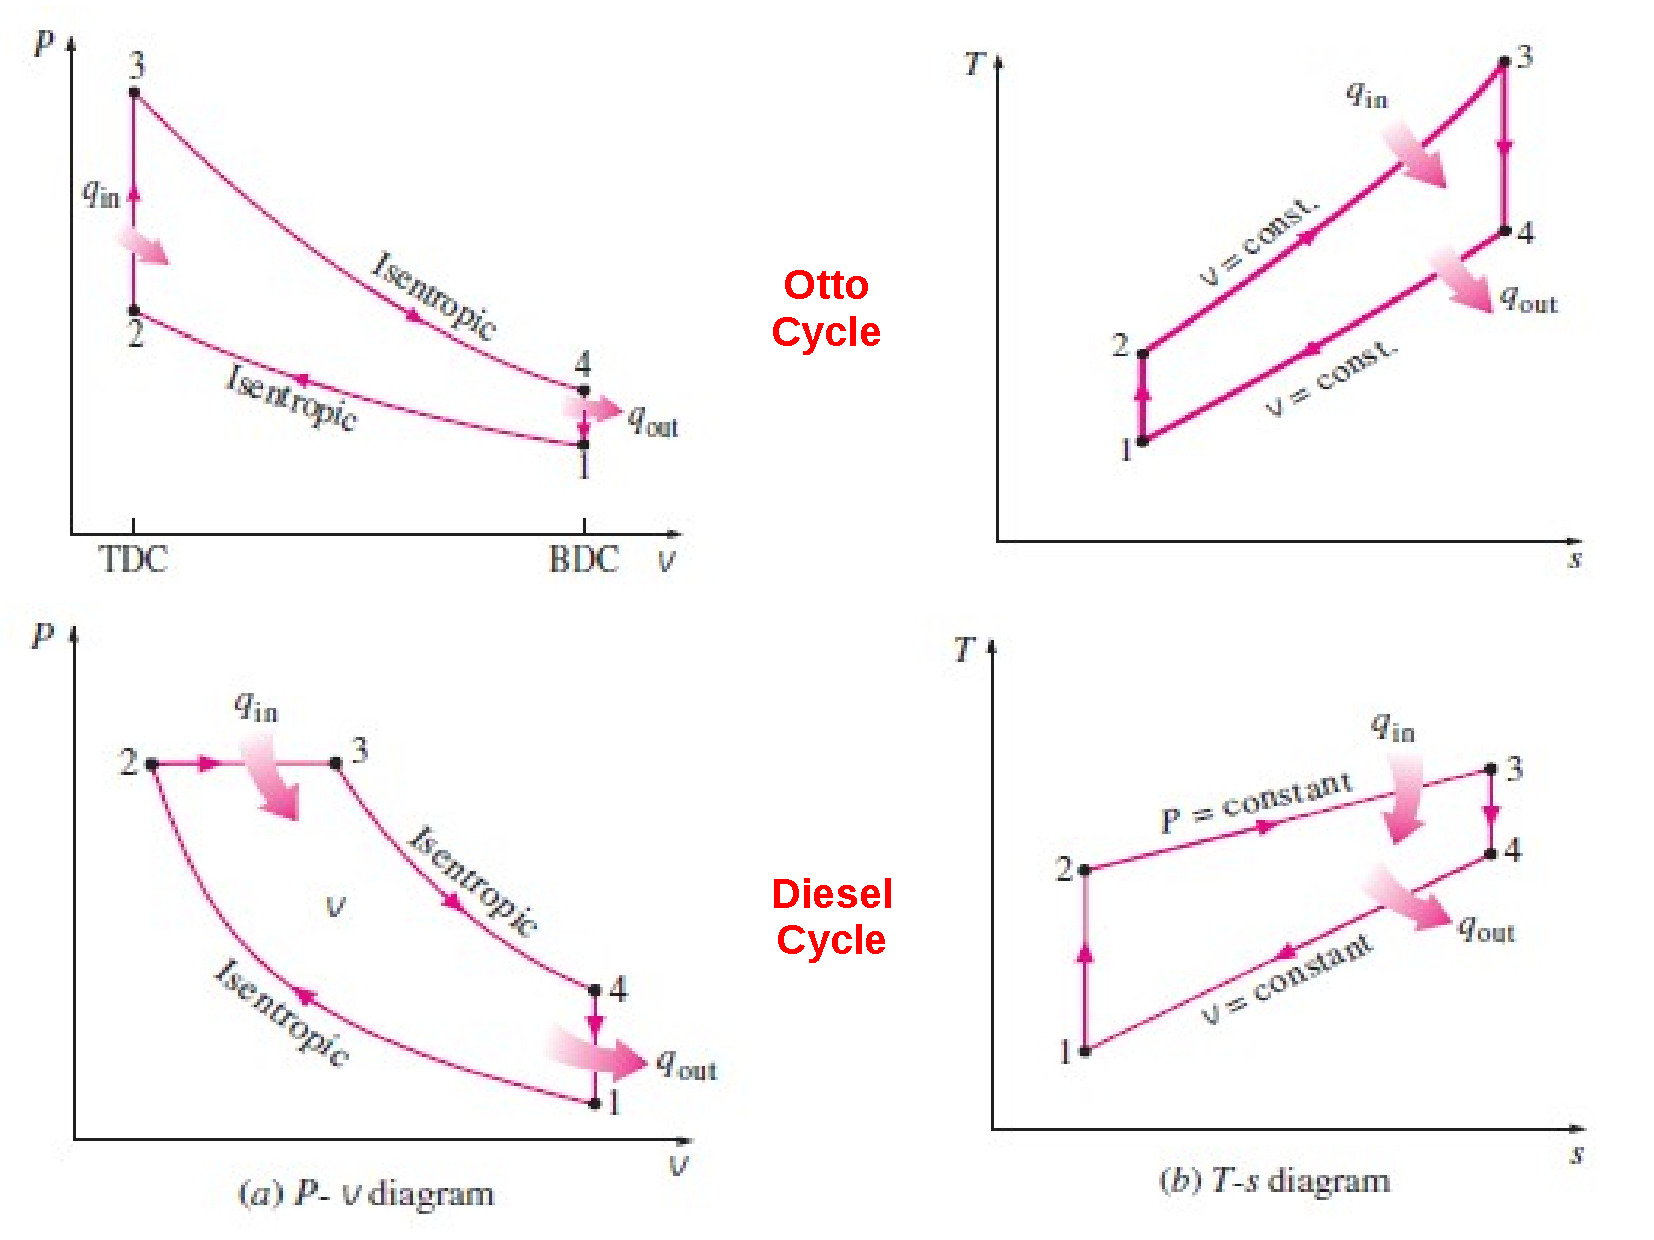
\includegraphics[width=10.cm,clip]{./Pics/InternalCombustion_IdealOttoxDieselCycles}
     \end{center}
    \end{figure}   
\end{frame}

%%%
%%% Slide
%%%
\begin{frame}
 \frametitle{Ideal Diesel Cycles}
  \begin{columns}
   \begin{column}[c]{0.5\linewidth}
    \begin{enumerate}\setcounter{enumi}{10}\scriptsize
     \item<1-> \blue{Assuming 1 kg of air:}
     \item<1-> Heat supplied at constant pressure: $Q_{s}=C_{p}\left(T_{3}-T_{2}\right)$;
     \item<1-> Heat rejected at constant volume: $Q_{r}=C_{v}\left(T_{4}-T_{1}\right)$;
     \item<1-> Work done: $W_{net}=C_{p}\left(T_{3}-T_{2}\right)-C_{v}\left(T_{4}-T_{1}\right)$.
     \item<2-> Efficiency: 
       \visible<2->{\begin{eqnarray}\scriptsize
         \eta_{\text{Diesel}}&=&\frc{C_{p}\left(T_{3}-T_{2}\right)-C_{v}\left(T_{4}-T_{1}\right)}{C_{p}\left(T_{3}-T_{2}\right)} \nonumber \\
                          &=& 1 - \frc{T_{4}-T_{1}}{\gamma\left(T_{3}-T_{2}\right)}
       \end{eqnarray}}
     \item<3-> For compression $\left(r\right)$ and \red{cut-off} ratios $\left(\rho\right)$:
       \visible<3->{\begin{displaymath}
           r=\frc{V_{1}}{V_{2}}\;\;\;\text{ and }\;\;\;\rho=\frc{\text{volume at cut-off}}{\text{clearence volume}}=\frc{V_{3}}{V_{2}}
       \end{displaymath}}
     \item<4-> Isentropic compression \textcolor{blue}{1--2}:
    \end{enumerate}
   \end{column}
   \begin{column}[c]{0.5\linewidth}\scriptsize
     \visible<4->{\begin{displaymath}\scriptsize
        \frc{T_{2}}{T_{1}}=\left(\frc{V_{1}}{V_{2}}\right)^{\gamma-1}=r^{\gamma-1} \Rightarrow T_{2}=T_{1}r^{\gamma-1}
     \end{displaymath}}
     \begin{enumerate}\setcounter{enumi}{16}\scriptsize
        \item<5-> Heat addition at constant pressure \blue{2-3}:
          \visible<5->{\begin{displaymath}
             \frc{T_{3}}{T_{2}}=\frc{V_{3}}{V_{2}}=\rho \Rightarrow T_{3}=\rho T_{2}=\rho T_{1} r^{\gamma-1}
          \end{displaymath}}
     \end{enumerate}
    \begin{figure}%
     \begin{center}
      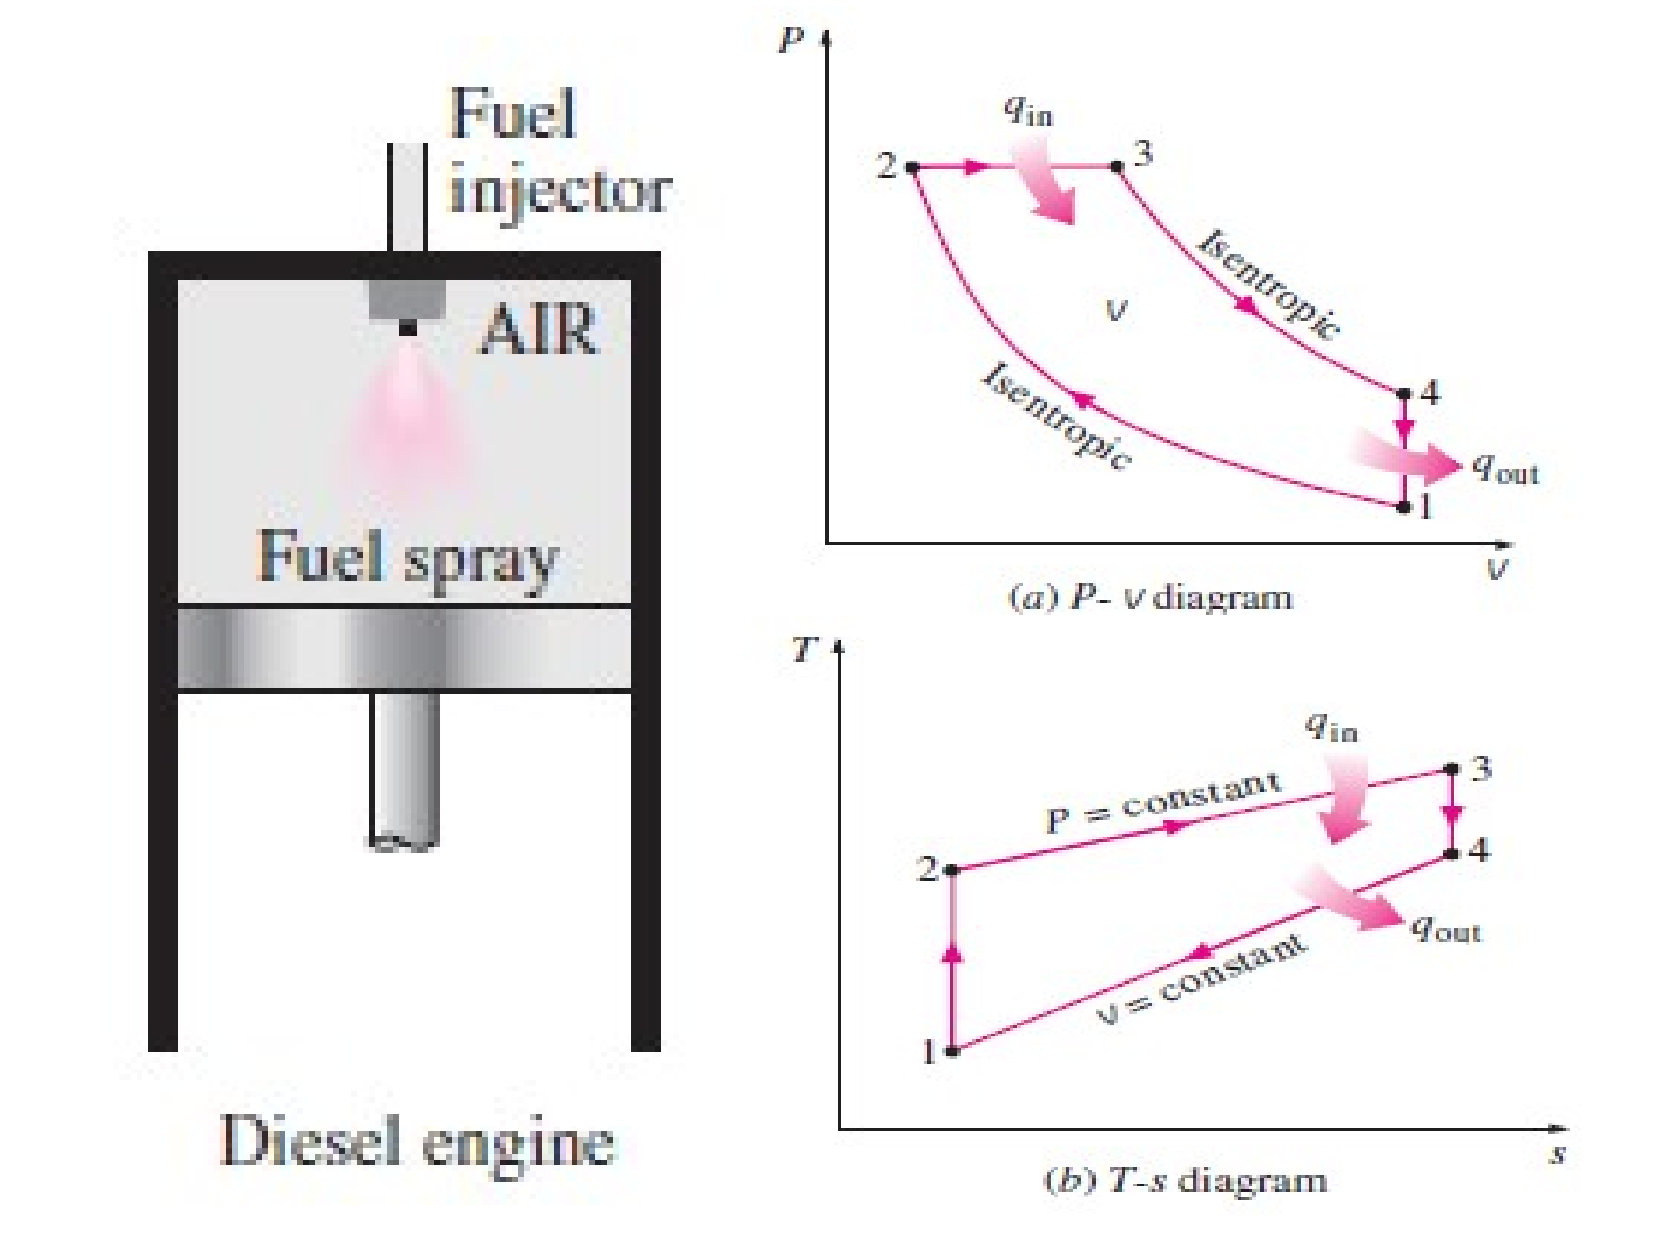
\includegraphics[width=4.cm,clip]{./Pics/InternalCombustion_IdealDieselCycle}
     \end{center}
    \end{figure}   
   \end{column}  
  \end{columns}
\end{frame}

%%%
%%% Slide
%%%
\begin{frame}
 \frametitle{Ideal Diesel Cycles}
    \begin{enumerate}\setcounter{enumi}{17}\scriptsize
       \item<1-> Isentropic expansion \blue{3-4}:
          \visible<1->{\begin{displaymath}
             \frc{T_{3}}{T_{4}} = \left(\frc{V_{4}}{V_{3}}\right)^{\gamma-1} = \left(\frc{V_{1}}{V_{3}}\right)^{\gamma-1}  = \left(\frc{V_{1}}{V_{2}}\frc{V_{2}}{V_{3}}\right)^{\gamma-1}= \left(\frc{r}{\rho}\right)^{\gamma-1} \Longrightarrow \;\; T_{4} = T_{1}\rho^{\gamma}
          \end{displaymath}}
       \item<2-> Replacing $T_{i}$ in the efficiency expression:
          \visible<2->{\begin{equation}
            \eta_{\text{Diesel}}= 1 - \frc{T_{4}-T_{1}}{\gamma\left(T_{3}-T_{2}\right)} = 1 - \frc{\rho^{\gamma}-1}{\gamma r^{\gamma-1}\left(\rho-1\right)} =  1 -\frc{1}{r^{\gamma-1}}\left[\frc{\rho^{\gamma}-1}{\gamma\left(\rho-1\right)}\right]
          \end{equation}}
       \item<3-> As $\eta_{\text{Otto}} =1 - \frc{1}{r^{\gamma-1}}$, it is clear that (as $\rho>1$) the term in square-brackets is always greater than 1, therefore;
       \item<4-> \blue{$\eta_{\text{Otto}} > \eta_{\text{Diesel}}$} when both cycles operates on the same compression ratio ($r$);
       \item<5-> \blue{Cut-off ratio} decreases  $\Rightarrow$ $\eta_{\text{Diesel}}$ increases;
       \item<6-> If $\rho\to 1$ (using \href{http://people.goshen.edu/~adecelles/calculus_notes/4_4_lhospitals_rule.pdf}{\blue{Calculus L'H\^opital rule}}) $\Rightarrow$ term in the square-bracket $\to$ 1 and \blue{$\eta_{\text{Otto}} = \eta_{\text{Diesel}}$}. 
       \item<7-> \textcolor{blue}{Net work} for diesel cycle can be define (as a function of $P$ and $V$) as,
         \visible<7->{\begin{displaymath}
            W_{\text{net}} = \displaystyle\frac{P_{1}V_{1}r^{\gamma-1}\left[\gamma\left(\rho-1\right)-r^{1-\gamma}\left(\rho^{\gamma}-1\right)\right]}{\gamma-1}
         \end{displaymath}}
       \item<8-> And the MEP can be expressed as
         \visible<8->{\begin{equation}
           MEP = \displaystyle\frac{P_{1}r^{\gamma}\left[\gamma\left(\rho-1\right)-r^{1-\gamma}\left(\rho^{\gamma}-1\right)\right]}{\left(\gamma-1\right)\left(r-1\right)}
         \end{equation}}
 \end{enumerate}
\end{frame}

%%%
%%% Slide
%%%
\begin{frame}
 \frametitle{Example 2: Diesel Engine (Problem 3)}
     An engine with 200 mm cylinder diameter and 300 mm stroke works on ideal Diesel cycle. The initial pressure and temperature of air are 1 bar and 27$^{\text{o}}$C, repectively. The cut-off is 8$\%$ of the stroke. Calculate: 
       \begin{enumerate}[(a)]
         \item pressures and temperatures at all stages; 
         \item theoretical air-standard efficiency; 
         \item MEP; 
         \item power of the engine if the working cycles per minute are 380. 
       \end{enumerate}
 Assume that the compression ratio ($r$) is 15 and the working fluid is air.
\end{frame}



%%%
%%% SECTION
%%%
\section{Brayton Gas-Turbine Cycles}


%%%===            ===%%%
%%%=== SUBSECTION ===%%%
%%%===            ===%%%
\subsection{Introduction}

%%%
%%% Slide
%%%
\begin{frame}
 \frametitle{Introduction}
 \begin{columns}
  \begin{column}[c]{0.6\linewidth} 
   \begin{enumerate}[(1)]\scriptsize
    \item<1-> Also called \blue{Joule cycle}, it is a \blue{constant pressure cycle} initially designed for perfect gasses;
    \item<2-> Gas turbines usually operate on an open cycle: 
    \item<2-> Fresh air at ambient conditions is drawn into the compressor, where the temperature and pressure are raised;
    \item<3-> The \blue{high-pressure air} stream is injected into the combustion chamber, where the \blue{fuel is burned at constant pressure}; 
    \item<3-> The \blue{high-temperature combustion gasses} are directed into the \blue{turbine} where they \blue{expand isentropically to the atmospheric pressure};
    \item<3-> The exhaust gases leaving the turbine are discarded (not recirculated) $\Longrightarrow$ \red{Open Cycle};
    \item<4-> However, we can simplify the open cycle by assuming \blue{air-standard} assumptions where;
    \item<4-> \blue{The combustion stage is replaced by a constant-pressure heat-addition stage from an external source} and;
    \item<4-> \blue{The exhaust stage is replaced by a constant-pressure heat-rejection stage to the ambient air}.
   \end{enumerate}
  \end{column}
  \begin{column}[c]{0.4\linewidth}
   \begin{figure}%
     \vbox{
        \visible<1->{\hbox{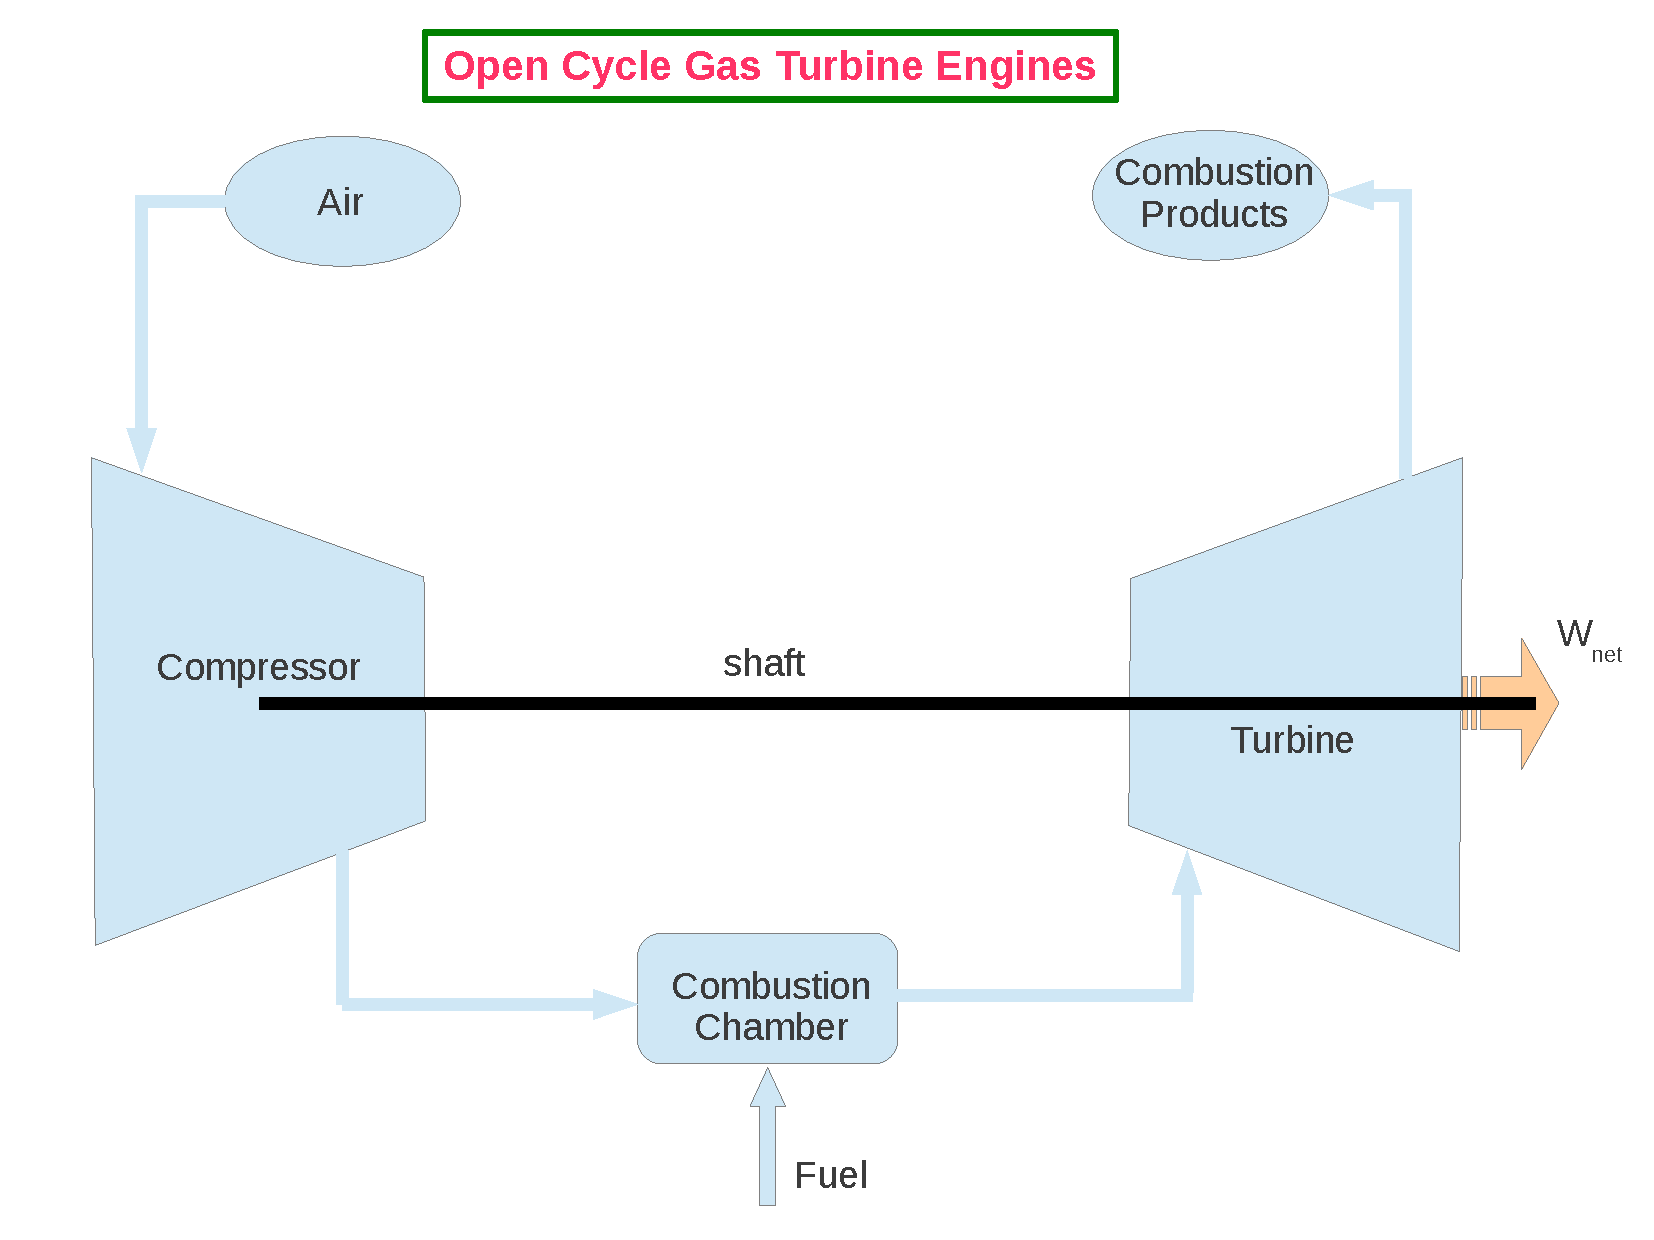
\includegraphics[width=3.8cm,clip]{./Pics/Open_Gas_Turbine_Engines} }}
        \visible<4->{\hbox{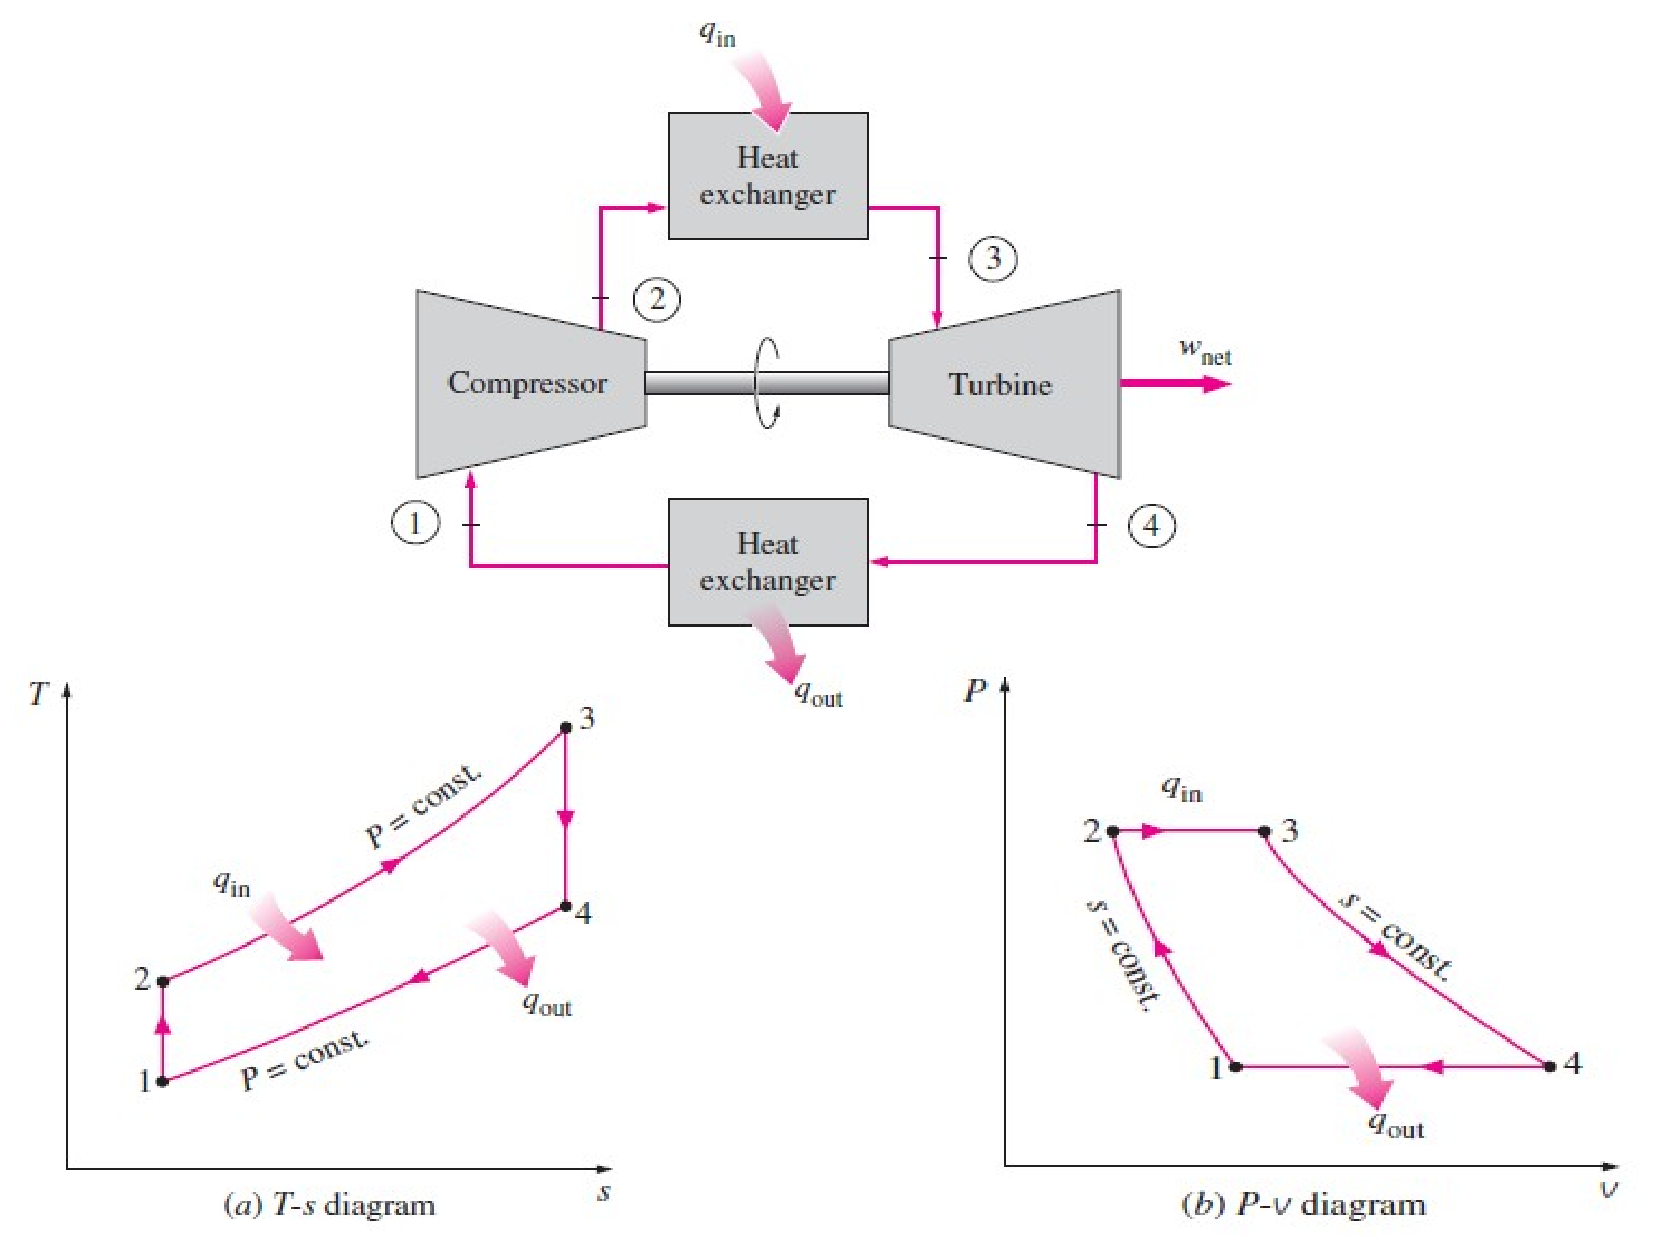
\includegraphics[height=4.5cm,width=4.5cm,clip]{./Pics/Brayton_cycle1}}}
     }
   \end{figure}  
  \end{column}  
 \end{columns}
\end{frame}



%%%===            ===%%%
%%%=== SUBSECTION ===%%%
%%%===            ===%%%
\subsection{Ideal Brayton Cycle}

%%%
%%% Slide
%%%
\begin{frame}
 \frametitle{Brayton Cycle -- Internally Reversible Processes}
 \begin{columns}
  \begin{column}[c]{0.5\linewidth} 
   \begin{enumerate}[(1)]\scriptsize
    \item<1-> Cycle (assuming 1 kg of air):
       \begin{enumerate}[(a)]\scriptsize
         \item<1->{\bf 1-2}: Isentropic compression of air (no heat flow);
         \item<2->{\bf 2-3}: Heat addition at constant pressure (heat flows into the system increasing the volume),
            \visible<2->{\begin{displaymath}
                 Q_{in} = C_{p}\left(T_{3}-T_{2}\right)
            \end{displaymath}}
         \item<3->{\bf 3-4}: Isentropic expansion (no heat flow);
         \item<4->{\bf 4-1}: Heat removal from the system at constant pressure (volume decreases), 
            \visible<4->{\begin{displaymath}
                 Q_{out} = C_{p}\left(T_{4}-T_{1}\right)
            \end{displaymath}}
       \end{enumerate}
    \item<5-> Net work:
       \visible<5->{\begin{displaymath}
           W_{\text{net}}=C_{p}\left[\left(T_{3}-T_{2}\right)-\left(T_{4}-T_{1}\right)\right]
       \end{displaymath}}
    \item<6-> Air-standard Brayton Efficiency:
   \end{enumerate}
  \end{column}
  \begin{column}[c]{0.5\linewidth}
    \begin{center}
   \begin{figure}%
     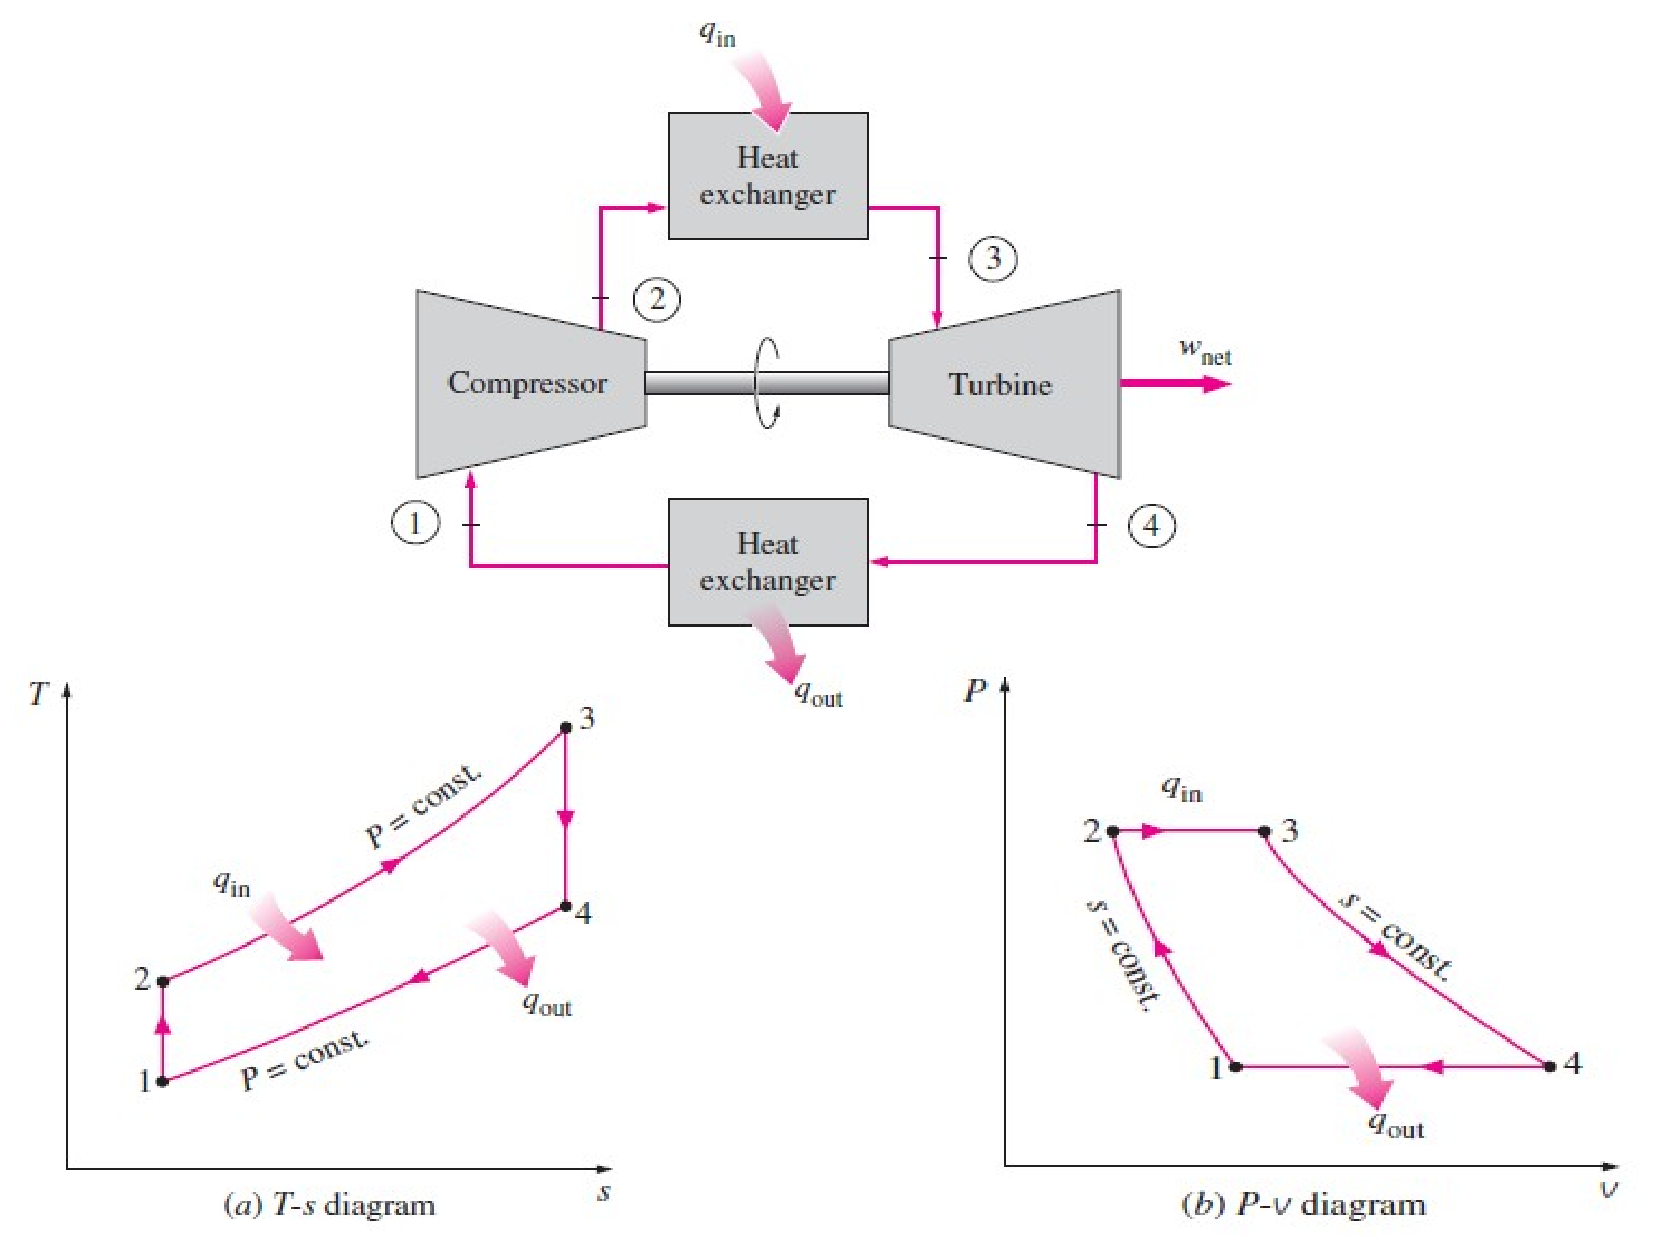
\includegraphics[height=5.cm,width=5.5cm,clip]{./Pics/Brayton_cycle1}
   \end{figure}  
    \end{center} 
       \scriptsize\visible<6->{\begin{equation}
          \scriptsize\eta_{\text{Brayton}}= \frc{\text{Net Work}}{\text{Heat Received}}= 1 - \frc{T_{3}-T_{1}}{T_{3}-T_{2}}\label{eqn:braytonefficiency}
       \end{equation}}
  \end{column}  
 \end{columns}
\end{frame}

%%%
%%% Slide
%%%
\begin{frame}
 \frametitle{Brayton Cycle -- Internally Reversible Processes}
 \begin{columns}
  \begin{column}[c]{0.5\linewidth} 
   \begin{enumerate}[(1)]\setcounter{enumi}{3}\scriptsize
    \item<1-> From the isentropic expansion (3-4) and compression (1-2), we can obtain $T_{2}$ and $T_{3}$:
       \visible<1->{\begin{displaymath}
          T_{2} = T_{1} r_{p}^{\left(\gamma-1\right)/\gamma} \text{ and } T_{3} = T_{4}r_{p}^{\left(\gamma-1\right)/\gamma}
       \end{displaymath}
       with pressure ratio $r_{p}=P_{2}/P_{1}$.}
    \item<2-> Replacing $T_{i}$ in the $\eta_{\text{Brayton}}$ expression (Eqn.~\ref{eqn:braytonefficiency}), we can rewrite the air-standard efficiency,
       \visible<2->{\begin{equation}
           \eta_{\text{Brayton}} = 1 - \frc{1}{r_{p}^{\left(\gamma-1\right)/\gamma}}
       \end{equation}}
    \item<3-> This expression shows that the \blue{efficiency} of the ideal Brayton cycle \blue{increases with the pressure ratio, $r_{p}$};
    \item<4-> Upper pressure limit is constrained by the limiting temperature of the material of the turbine:
   \end{enumerate}
  \end{column}
  \begin{column}[c]{0.5\linewidth}
    \begin{center}
   \begin{figure}%
     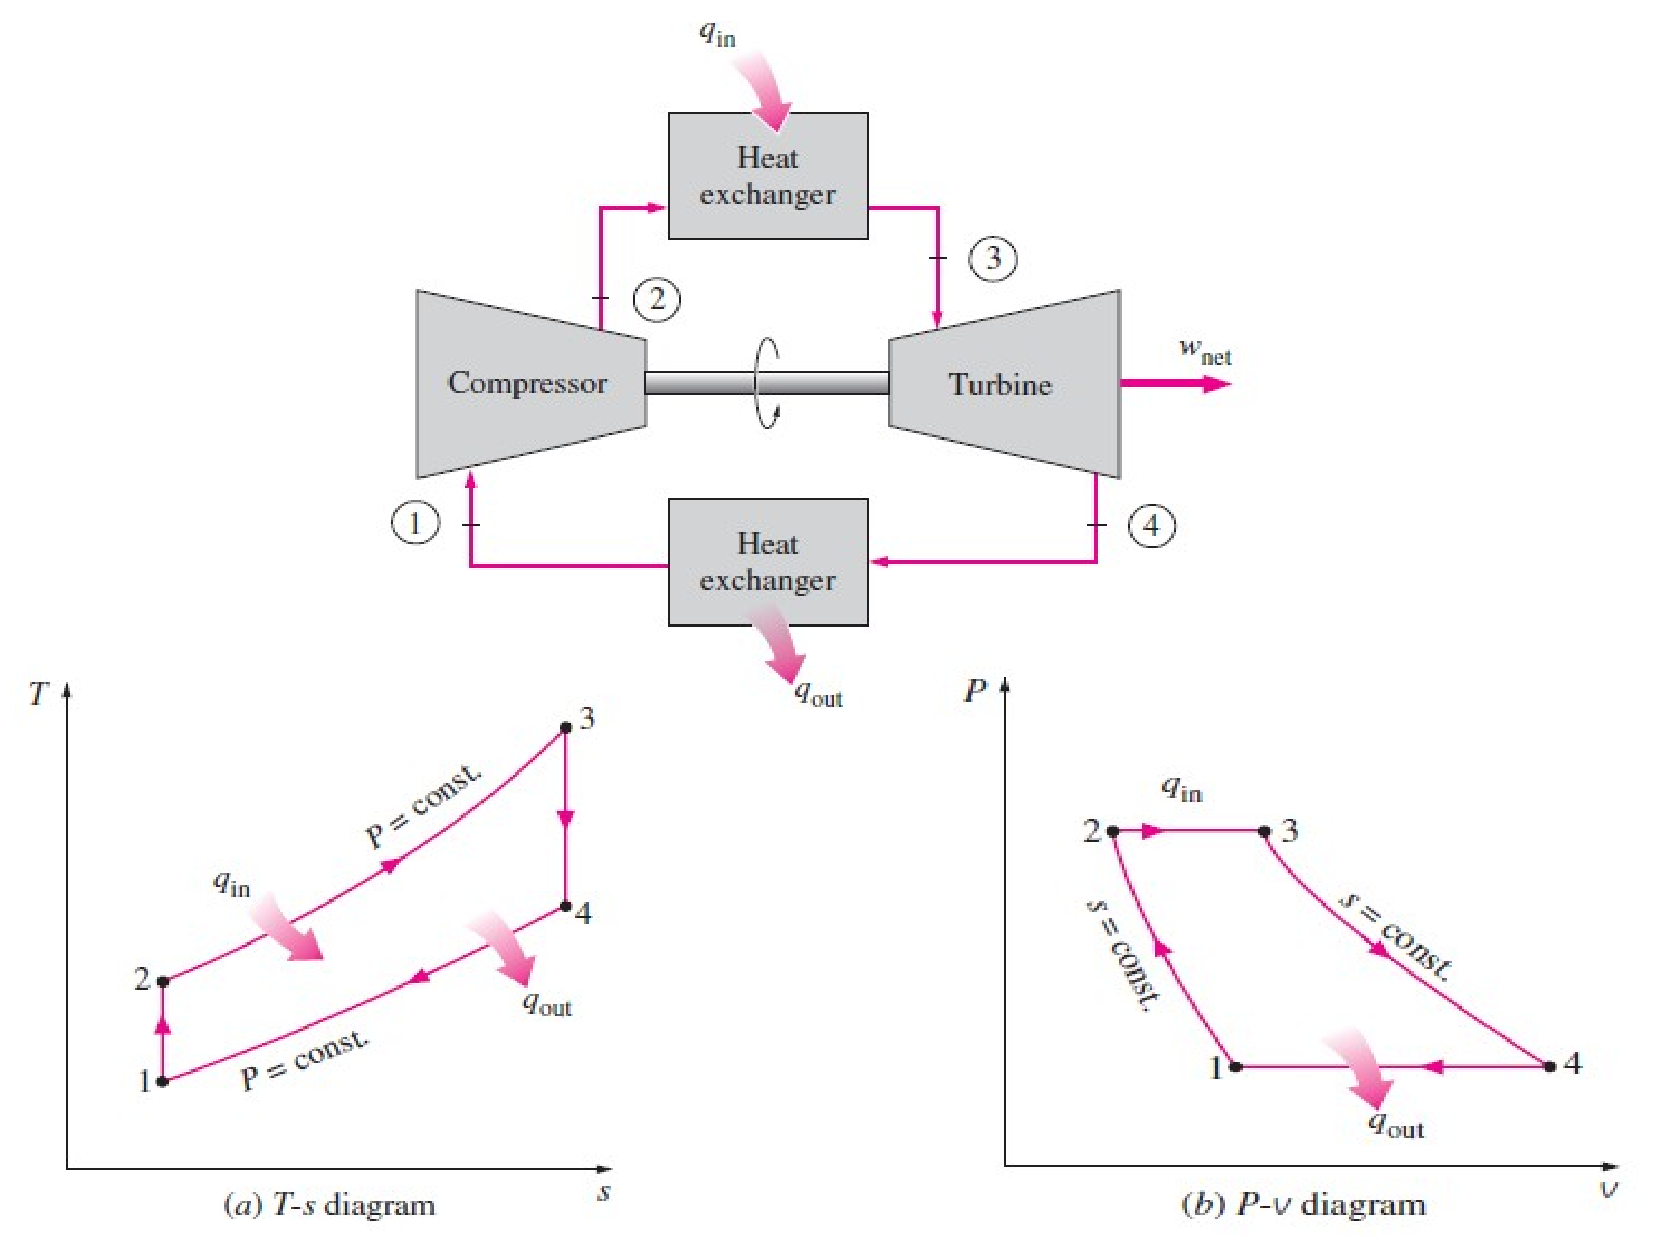
\includegraphics[height=5.cm,width=5.5cm,clip]{./Pics/Brayton_cycle1}
   \end{figure}  
    \end{center} 
  \end{column}  
 \end{columns}
       \visible<4->{\begin{center}
          \scriptsize\blue{Thermodynamics} $\Longleftrightarrow$ \green{Heat Transfer}  $\Longleftrightarrow$ \red{Material Sciences}
       \end{center}}
\end{frame}



%%%
%%% Slide
%%%
\begin{frame}
 \frametitle{Brayton Cycle -- Thermal Analysis}
 \begin{columns}
  \begin{column}[c]{0.5\linewidth} 
   \begin{enumerate}[(1)]\setcounter{enumi}{7}\scriptsize
    \item<1-> We can easily prove it by using the previously defined net work $\left(W_{\text{net}}\right)$:
       \visible<1->{\begin{eqnarray}
            W_{\text{net}}&=&C_{p}\left[\left(T_{3}-T_{2}\right)-\left(T_{4}-T_{1}\right)\right]\nonumber \\
                   &=&C_{p}\left[\left(T_{3}-T_{4}\right)-\left(T_{2}-T_{1}\right)\right] \nonumber \\
                   &=&C_{p}\left[T_{3}\left(1-\frc{T_{4}}{T_{3}}\right)-T_{1}\left(\frc{T_{2}}{T_{1}}-1\right)\right] \nonumber
       \end{eqnarray}}
    \item<2-> Since $\frc{T_{3}}{T_{4}}=r_{p}^{\left(\gamma-1\right)/\gamma}=\frc{T_{2}}{T_{1}}$, assuming $\gamma$ is constant and defining $\phi=\frc{\gamma-1}{\gamma}$,
        \visible<2->{\begin{displaymath}
           W_{\text{net}} = C_{p}\left[T_{3}\left(1-r_{p}^{-\phi}\right)-T_{1}\left(r_{p}^{\phi}-1\right)\right]
        \end{displaymath}}
    \item<3-> In order to obtain the \red{maximum net work}, we should differentiate $W_{\text{net}}$ with respect to $r_{p}$,
        \visible<2->{\begin{displaymath}
            \frc{d}{d r_{p}}W_{\text{net}}= C_{p} \left[ T_{3} \frc{\phi}{r_{p}\left(\phi+1\right)}-T_{1}\phi r_{p}^{\phi-1}\right]=0
        \end{displaymath}}
   \end{enumerate}
  \end{column}
  \begin{column}[c]{0.5\linewidth}
    \begin{center}
   \begin{figure}%
     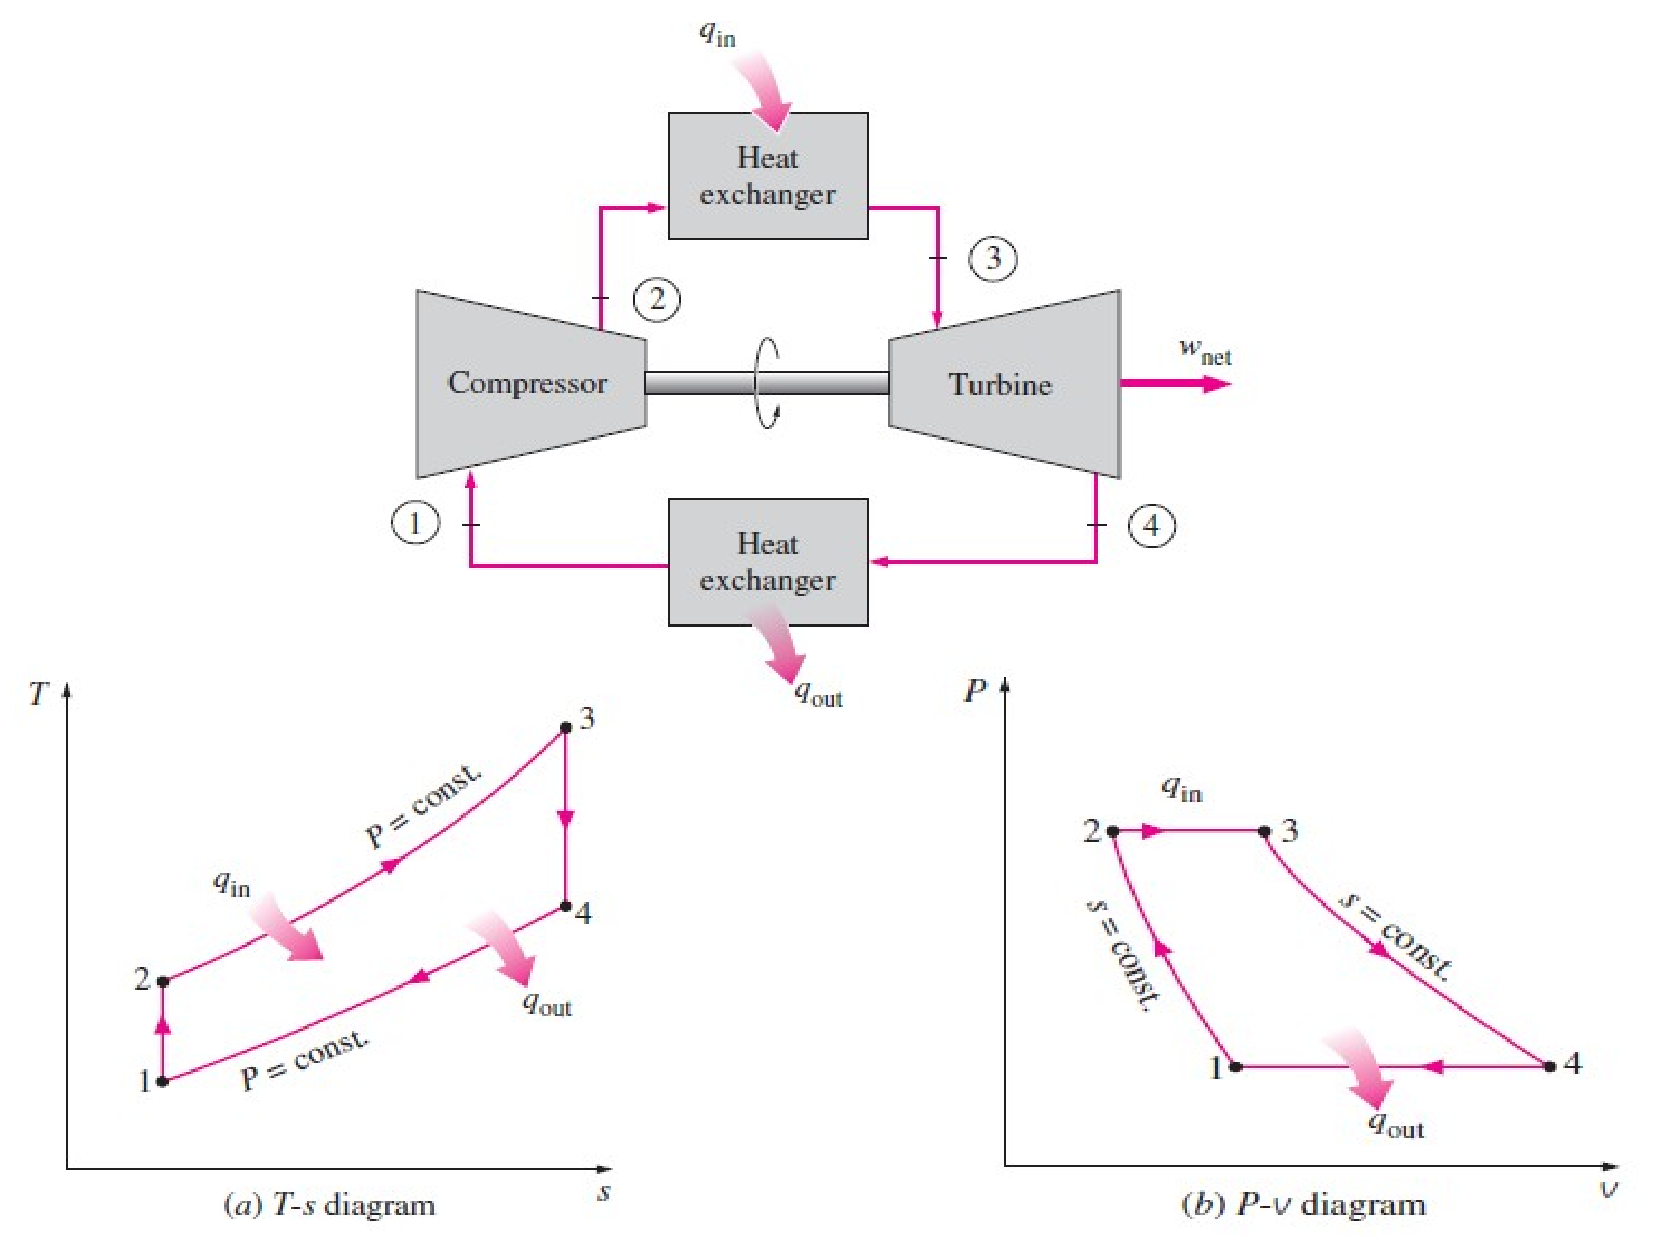
\includegraphics[height=5.cm,width=5.5cm,clip]{./Pics/Brayton_cycle1}
   \end{figure}  
    \end{center} 
  \end{column}  
 \end{columns}
\end{frame}

%%%
%%% Slide
%%%
\begin{frame}
 \frametitle{Thermal Analysis}
 \begin{columns}
  \begin{column}[c]{0.4\linewidth} 
    \begin{enumerate}[(1)]\setcounter{enumi}{10}\scriptsize
       \item<1-> This expression can be simplified to 
         \visible<1->{\begin{displaymath}
             r_{p}=\left(\frc{T_{3}}{T_{1}}\right)^{\frc{\gamma}{2\left(\gamma-1\right)}}
         \end{displaymath}}
       \item<2-> With $T_{1}$ being the minimum temperature of the system (i.e., inlet compressor temperature) and $T_{3}$ the maximum temperature that the turbine is able to withstand;
       \item<2-> For design purposes, we need to compromise between $r_{p}$ $\left(\text{and therefore }\eta_{\text{Brayton}}\right)$ and the net work output;
       \item<2-> With less work output per cycle $\Rightarrow$ Larger mass flow rate $\Rightarrow$ Larger system (for the same power output) $\Rightarrow$ More expensive.
    \end{enumerate}
  \end{column}
  \begin{column}[c]{0.6\linewidth}
    \begin{center}
   \begin{figure}%
     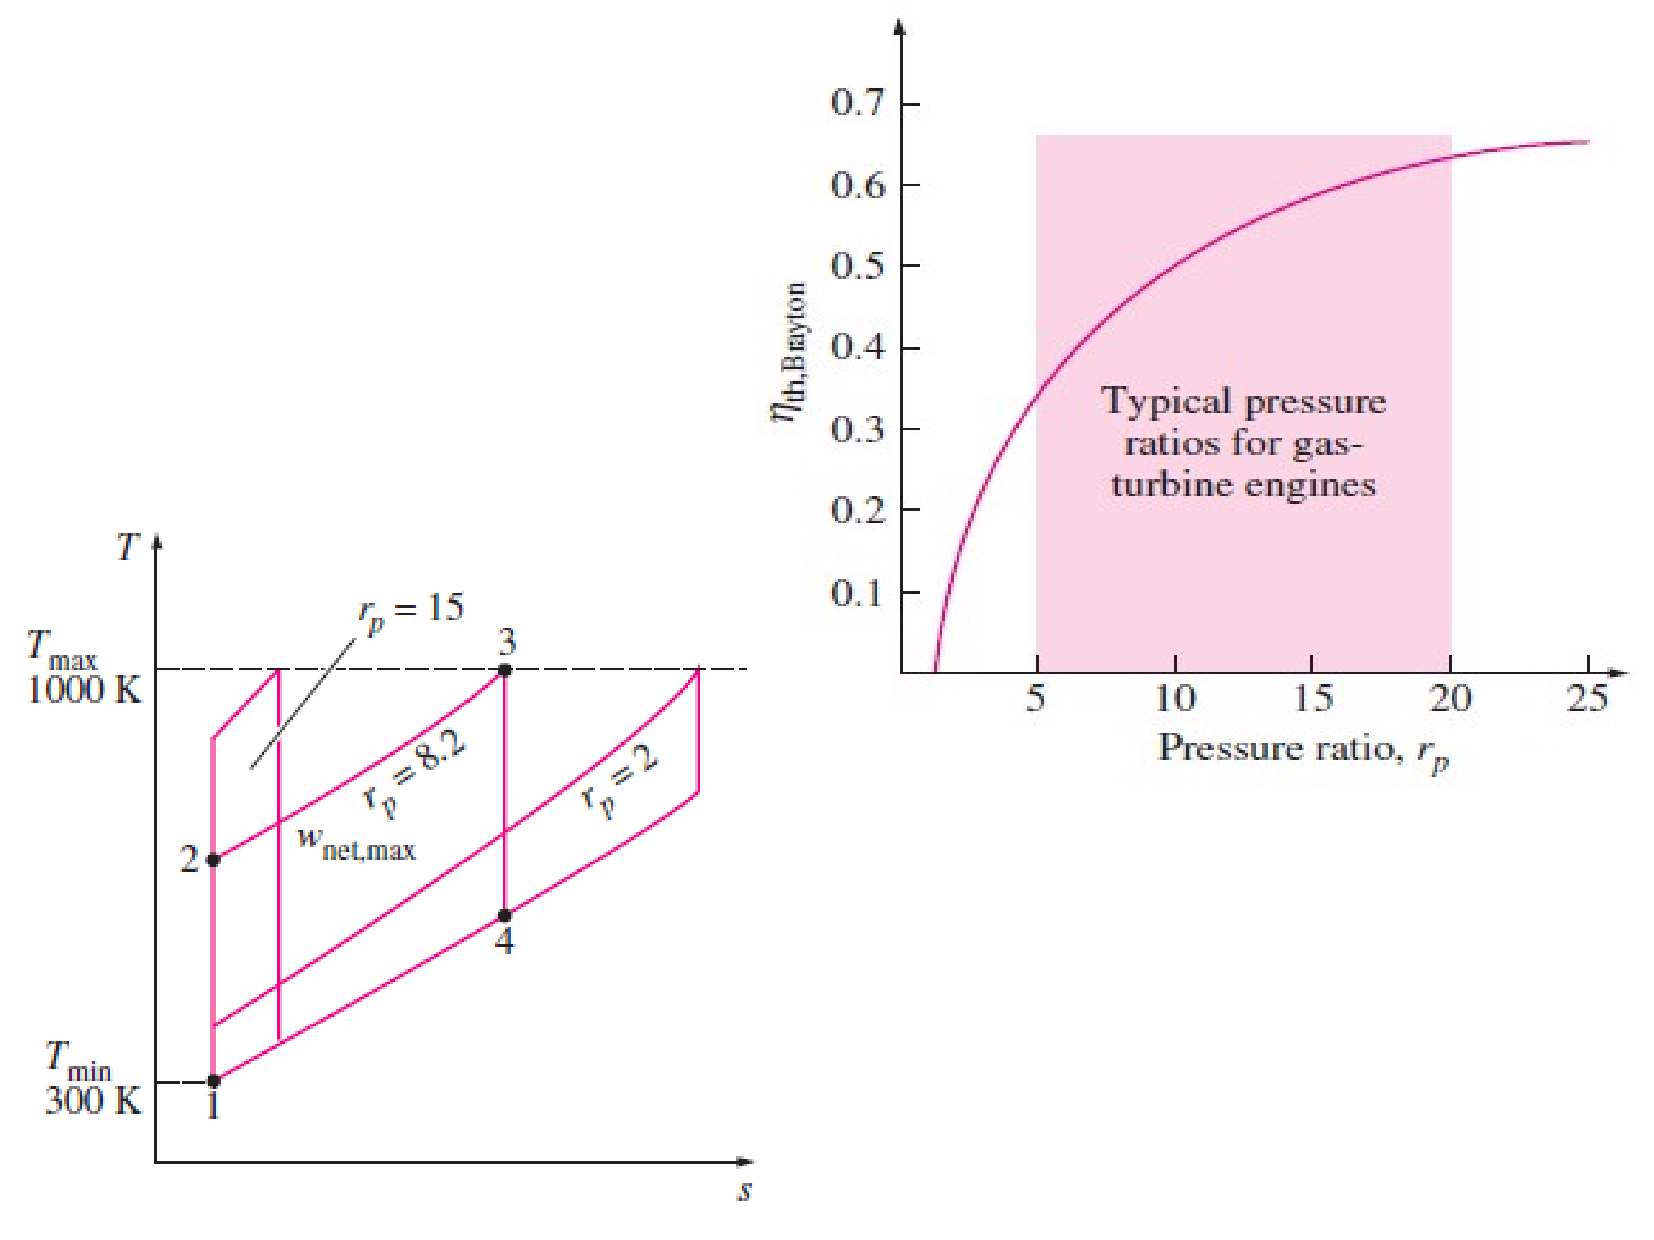
\includegraphics[height=6.cm,width=6.5cm,clip]{./Pics/Brayton_cycle2}
   \end{figure}  
    \end{center}
  \end{column}  
 \end{columns}
\end{frame}



%%%===            ===%%%
%%%=== SUBSECTION ===%%%
%%%===            ===%%%
\subsection{Actual Brayton Cycle}

%%%
%%% Slide
%%%
\begin{frame}
 \frametitle{Open Gas Turbine Cycle}
 \begin{columns}
  \begin{column}[c]{0.6\linewidth} 
    \begin{enumerate}[(1)]\scriptsize
      \item<1-> \red{Real Gas Turbines operate on Open Cycle};
      \item<2-> A rotary compressor and a turbine are mounted on a common shaft;
      \item<2-> Air is driven into a compressor and pumped into a combustion chamber;
      \item<2-> Energy is supplied by spraying fuel into the air stream and;
      \item<2-> The resulting hot gases expand through the turbine to the atmosphere.
      \item<3-> In order to obtain a net work output from the unit, the turbine must develop more gross work output than is required to drive the compressor and to overcome mechanical losses in the drive;
      \item<3-> \underline{The products of combustion coming out from the turbine} \underline{are exhausted to the atmosphere} as they cannot be reused. The working fluids (air and fuel) must be continuously replaced;
      \item<4-> If we neglect the pressure loss in the combustion chamber, the actual cycle becomes:
         \begin{enumerate}[(a)]\scriptsize
             \item<4-> \blue{1--2$^{\prime}$} Irreversible adiabatic compression
             \item<4-> \blue{2$^{\prime}$--3} Constant pressure heat supply in the combustion chamber;
             \item<4-> \blue{3--4$^{\prime}$} Irreversible adiabatic expansion;
             %\item<4-> \blue{1--2} Ideal isentropic compression and;
             %\item<4-> \blue{3--4} Ideal isentropic expansion.
        \end{enumerate}
 \end{enumerate}
  \end{column}
  \begin{column}[c]{0.4\linewidth}
    \begin{center}
   \begin{figure}%
     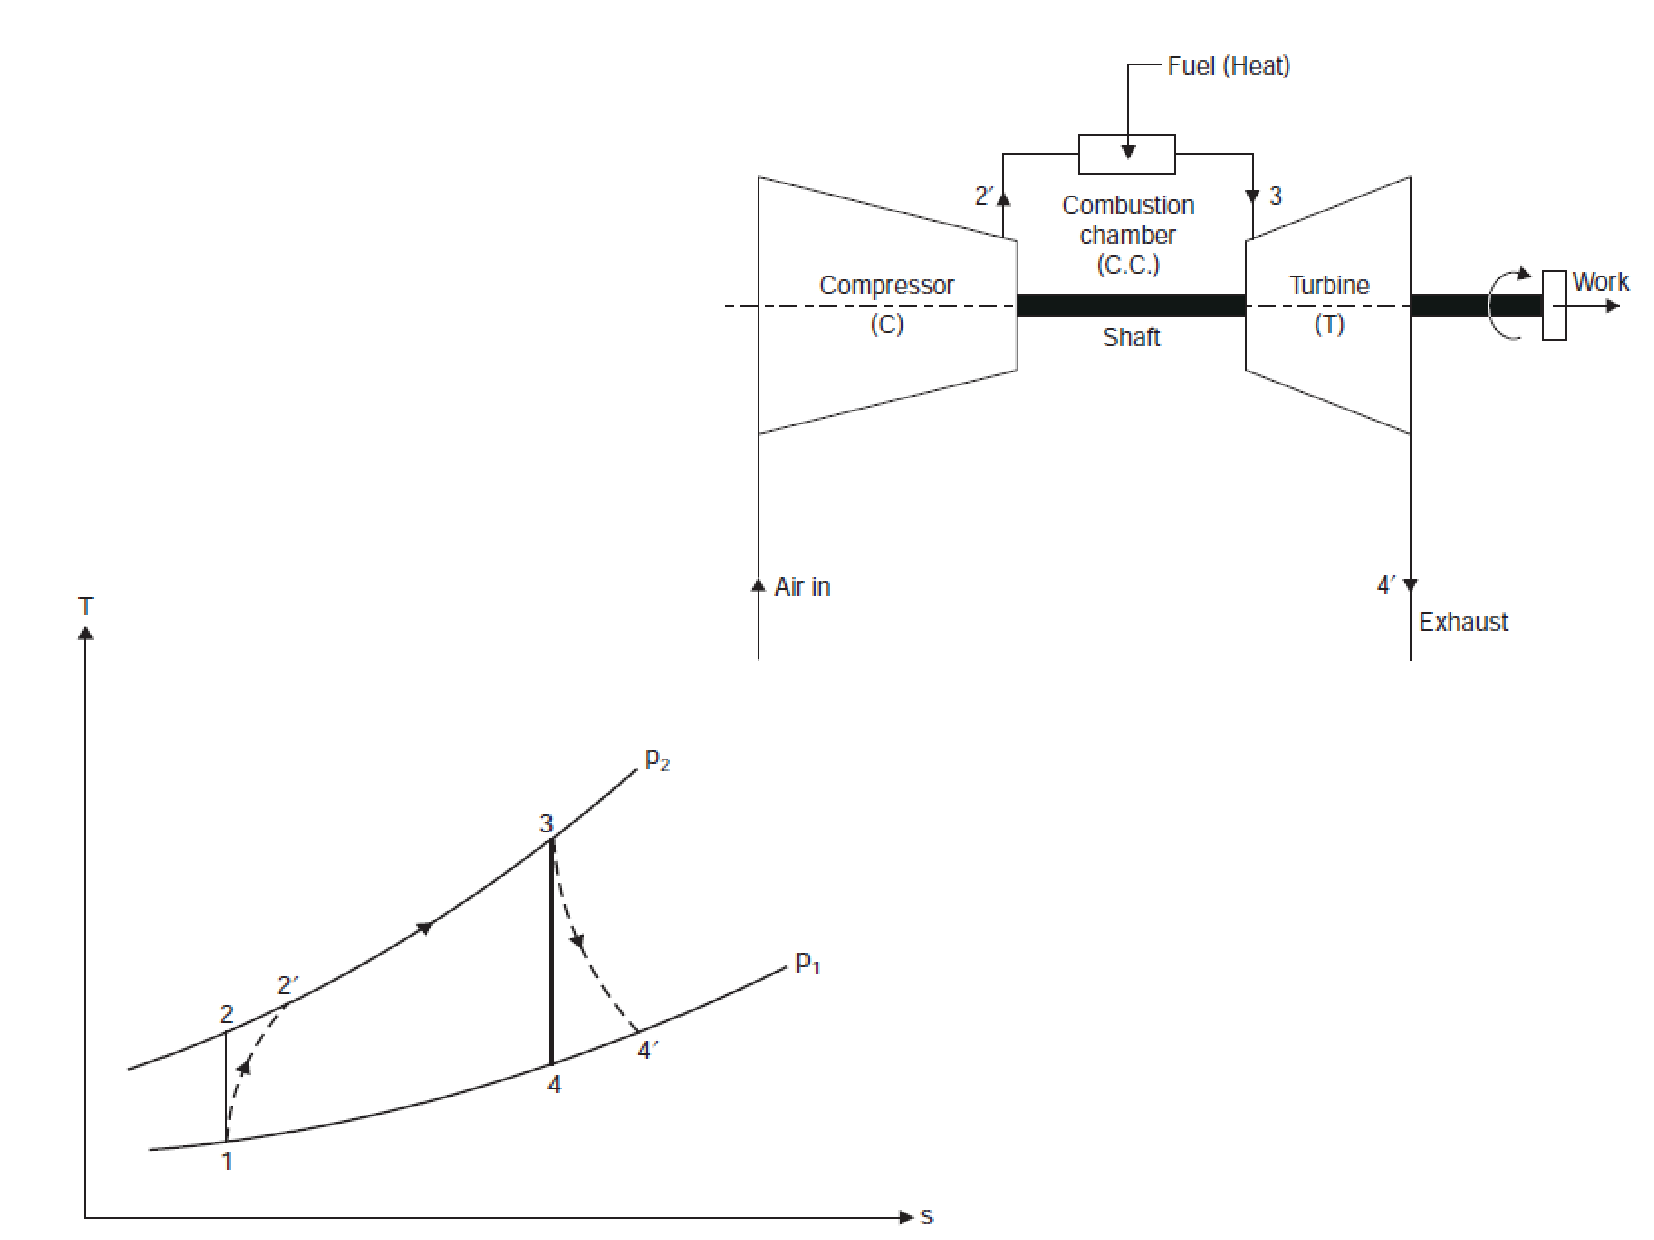
\includegraphics[height=5.cm,width=4.5cm,clip]{./Pics/Brayton_cycle3}
   \end{figure}  
    \end{center}
  \end{column}  
 \end{columns}
\end{frame}


%%%
%%% Slide
%%%
\begin{frame}
 \frametitle{Open Gas Turbine Cycle}
 \begin{columns}
  \begin{column}[c]{0.5\linewidth} 
    \begin{enumerate}[(1)]\setcounter{enumi}{8}\scriptsize
      \item<1-> \blue{We can still simplify the system by assuming that the change in the kinetic energy in various stages of the cycle is negligible if compared with the enthalpies changes;}
      \item<2-> Work input in the compressor: $C_{p}\left(T_{2}^{\prime}-T_{1}\right)$
      \item<2-> Heat supplied in the combustion chamber: $C_{p}\left(T_{3}-T_{2}^{\prime}\right)$
      \item<2-> Work output from the turbine: $C_{p}\left(T_{3}-T_{4}^{\prime}\right)$
      \item<2-> Net work: $W_{\text{net}}=C_{p}\left[\left(T_{3}-T_{4}^{\prime}\right) - \left(T_{2}^{\prime}-T_{1}\right)\right]$
      \item<3-> Thermal efficiency,
         \visible<3->{\begin{equation}
            \eta_{\text{Brayton}}^{\text{actual}} = \frc{\left(T_{3}-T_{4}^{\prime}\right) - \left(T_{2}^{\prime}-T_{1}\right)}{T_{3}-T_{2}^{\prime}}
         \end{equation}}
      \item<4-> Efficiency of the isentropic compressor:
         \visible<4->{\begin{eqnarray}
            \eta_{\text{Comp}}&=&\frc{\text{Work input in the isentropic compressor}}{\text{Actual work required}} \nonumber \\
                                          &=& \frc{T_{2}-T_{1}}{T_{2}^{\prime}-T_{1}}
         \end{eqnarray}}
 \end{enumerate}
  \end{column}
  \begin{column}[c]{0.4\linewidth}
    \begin{enumerate}[(1)]\setcounter{enumi}{15}\scriptsize
      \item<5-> Efficiency of the isentropic turbine:
         \visible<5->{\begin{eqnarray}
            \eta_{\text{Turb}} &=& \frc{\text{Actual work output}}{\text{Isentropic work output}} \nonumber \\
                                          &=& \frc{T_{3}-T_{4}^{\prime}}{T_{3}-T_{4}}
         \end{eqnarray}}
    \end{enumerate}\vspace{-.8cm}
    \begin{center}
   \begin{figure}%
     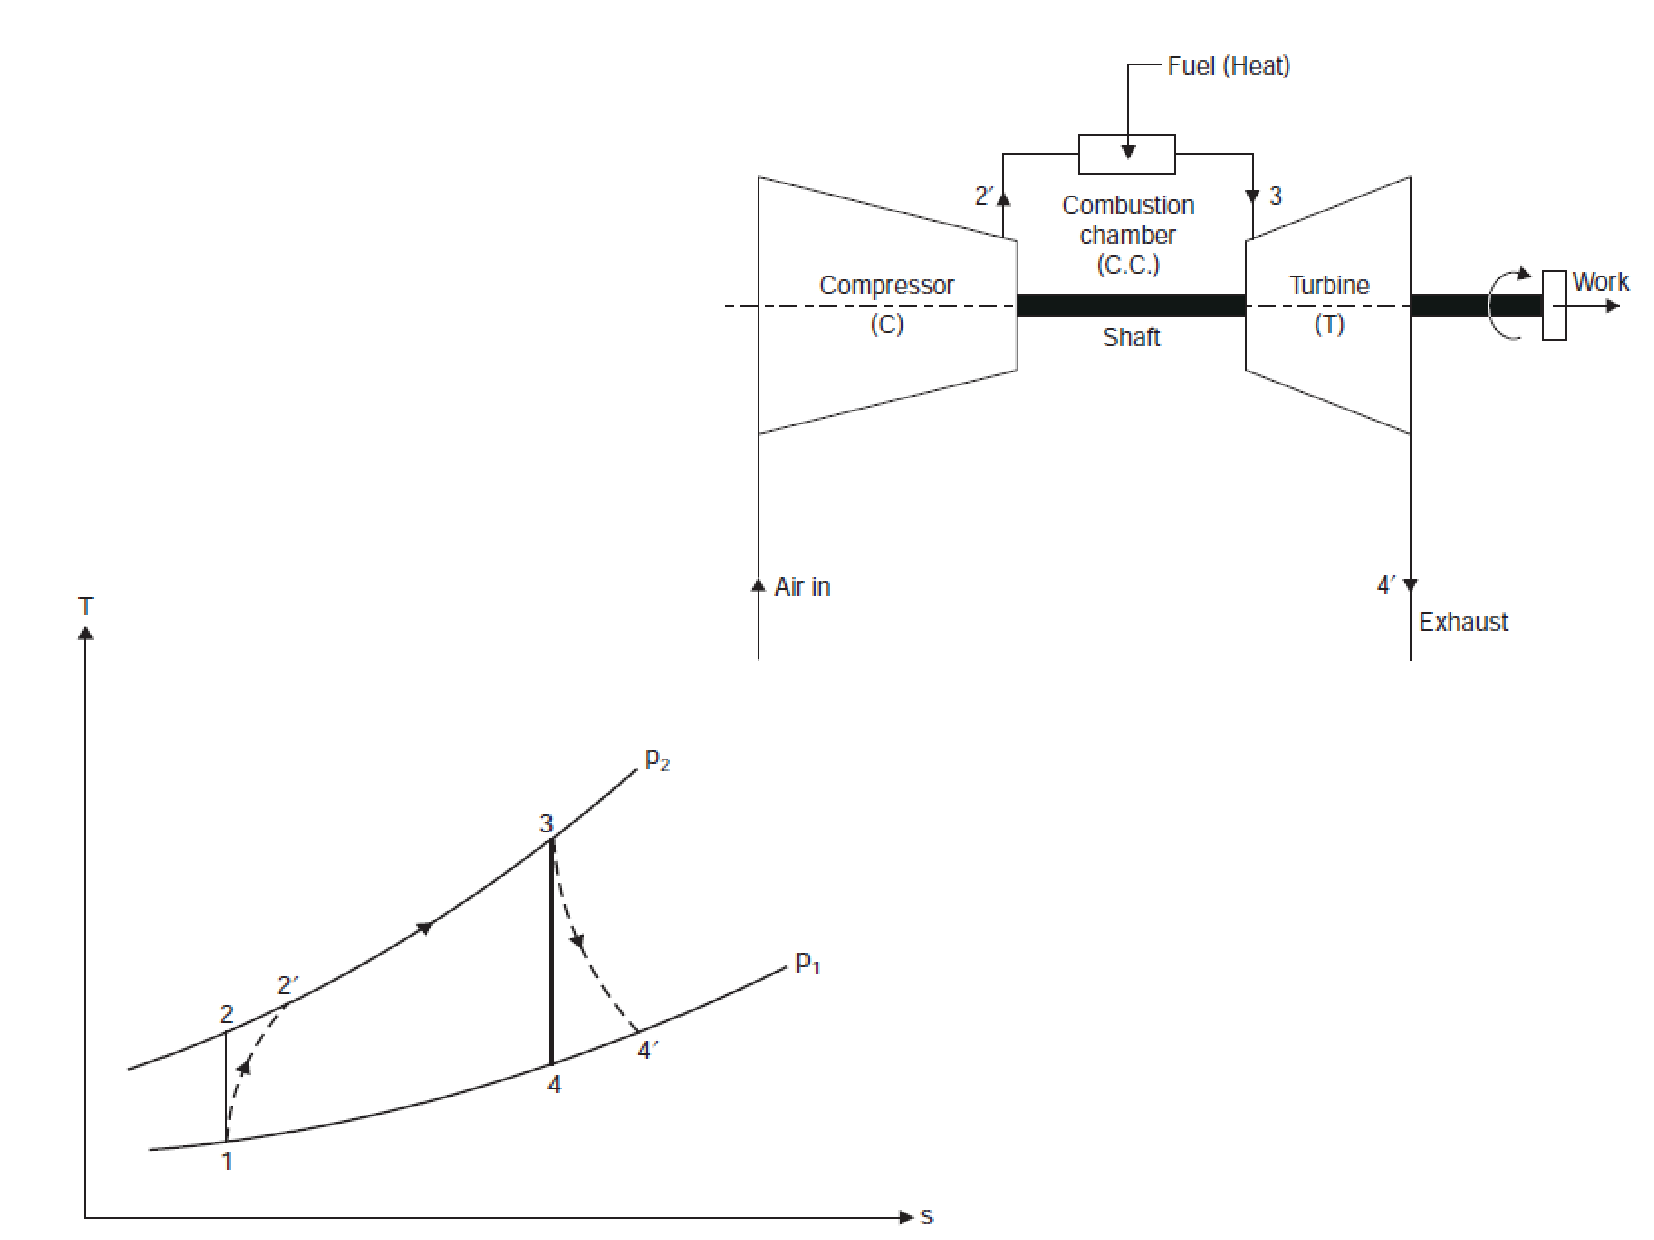
\includegraphics[height=4.5cm,width=4.5cm,clip]{./Pics/Brayton_cycle3}
   \end{figure}  
    \end{center}
  \end{column}  
 \end{columns}
\end{frame}

%%%
%%% Slide
%%%
\begin{frame}
 \frametitle{Improving the Efficiency: Brayton Cycle with Regeneration}
 \begin{columns}
   \begin{column}[c]{0.5\linewidth} 
      \begin{enumerate}[(1)]\scriptsize
        \item<1-> Temperature of the exhaust gasses leaving the turbine, $T_{4}$ is higher than the temperature leaving the compressor $T_{2}$ leading the combustion chamber;
        \item<2-> In order to improve the efficiency of the cycle we can use part of the heat from the $T_{4}$ fluid stream to increase the temperature of flow leaving the compressor;
        \item<3-> To this end, we can use a \textcolor{blue}{counter-flow heat exchanger}. This is also known as \textcolor{blue}{regenerator} or \textcolor{blue}{recuperator}.
        \item<4-> Notice that $T_{5^{\prime}}=T_{4}>T_{5}$
        \item<4-> The extent to which a regenerator approaches an ideal regenerator is called \textcolor{blue}{effectiveness}, $\varepsilon$
          \begin{displaymath}
             \varepsilon=\frc{Q_{\text{Regen}}^{\text{act}}}{Q_{\text{Regen}}^{\text{max}}} = \frc{h_{5}-h_{2}}{h_{4}-h_{2}}
          \end{displaymath}
        \item<5-> If we use the air-standard assumptions, the expression above becomes,
          \begin{displaymath}
            \varepsilon= \frc{T_{5}-T_{2}}{T_{4}-T_{2}}
          \end{displaymath}  
       \end{enumerate}
  \end{column}
  \begin{column}[c]{0.5\linewidth}
    \begin{center}
   \begin{figure}%
     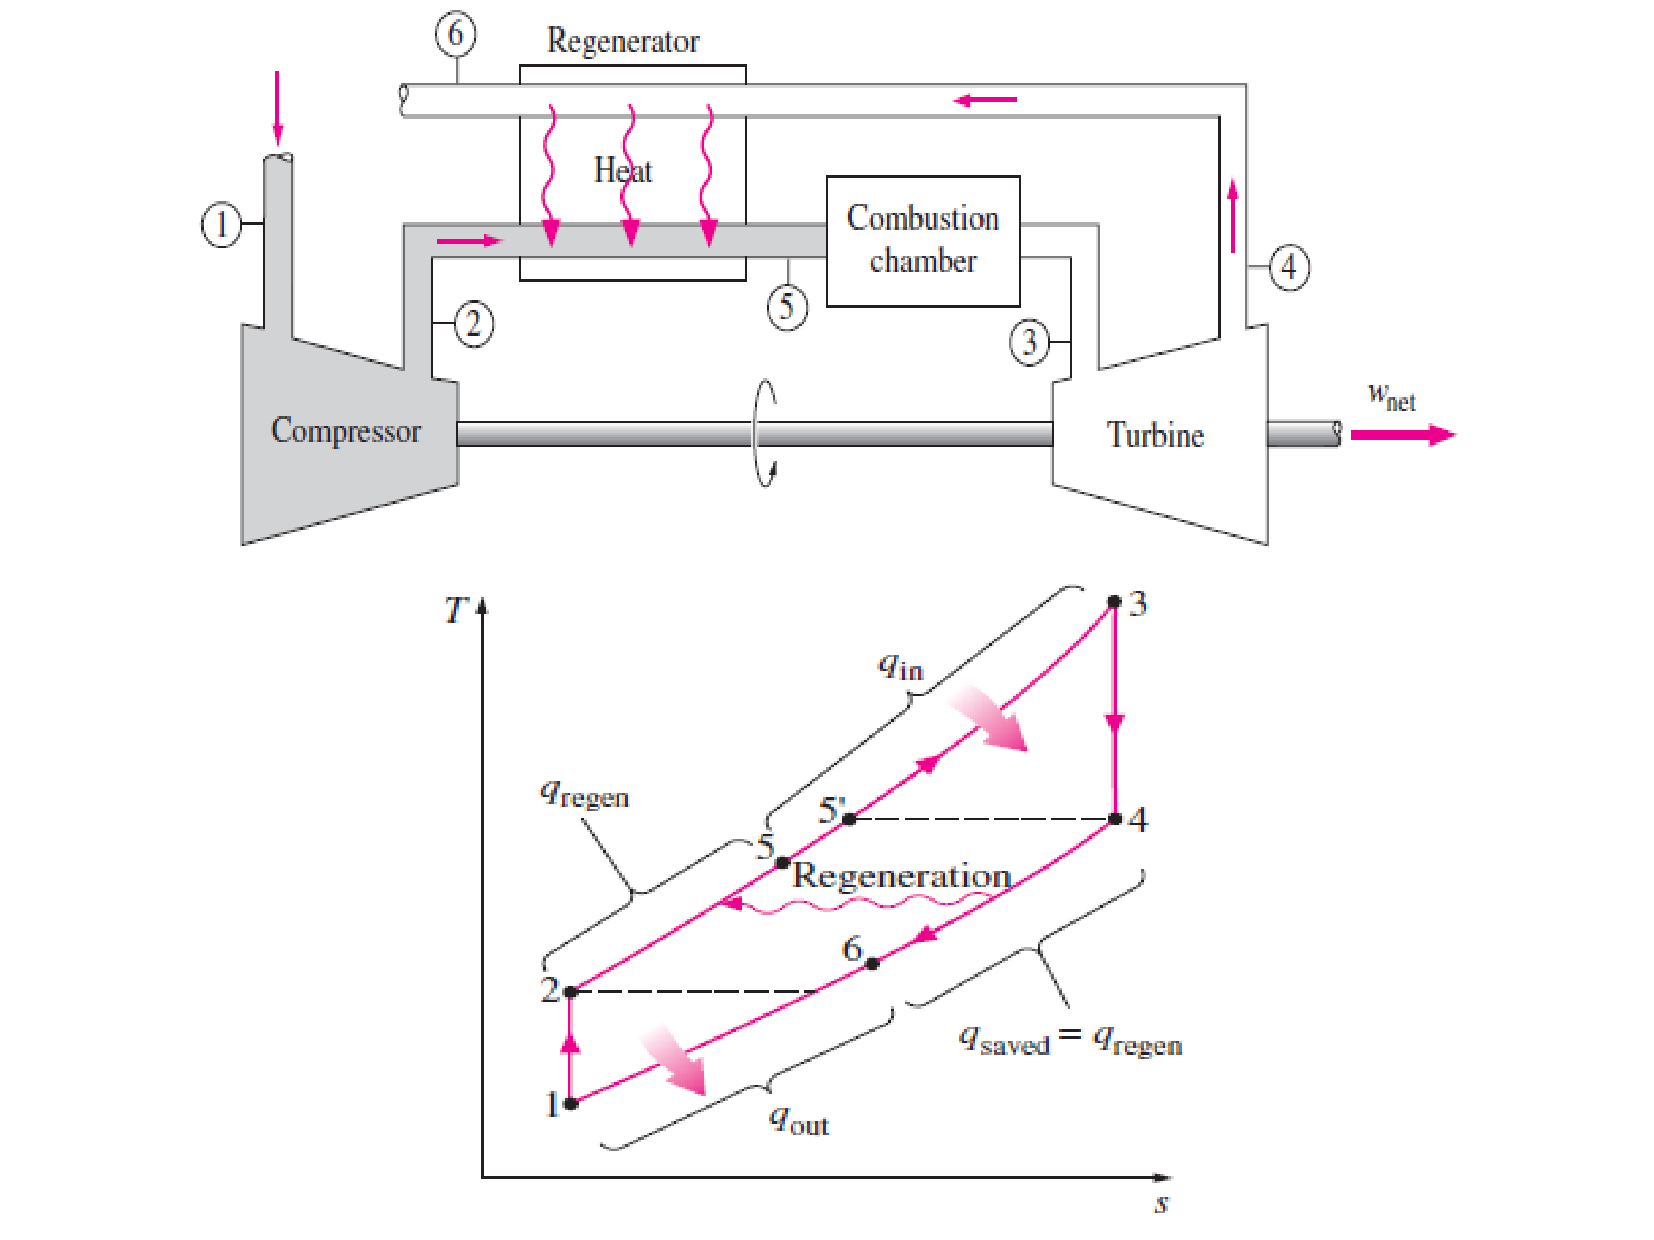
\includegraphics[height=5.cm,width=4.5cm,clip]{./Pics/Brayton_cycle4}
   \end{figure}  
    \end{center}
  \end{column}  
 \end{columns}
\end{frame}


%%%
%%% Slide
%%%
\begin{frame}
 \frametitle{Improving the Efficiency: Brayton Cycle with Regeneration}
 \begin{columns}
   \begin{column}[c]{0.5\linewidth} 
      \begin{enumerate}[(1)]\setcounter{enumi}{6}\scriptsize
        \item<1-> A regenerator with a higher effectiveness obviously saves a greater amount of fuel since it preheats the air to a higher temperature prior to combustion;
        \item<1-> The effectiveness of most regenerators used in practice is below 0.85;
        \item<2-> The thermal efficiency of the Brayton cycle with regenerator is
           \begin{equation}
             \eta_{\text{Brayton}}^{\text{Regen}}= 1 - \left[\frc{T_{1}}{T_{3}}\right] r_{p}^{\left(\gamma-1\right)/\gamma}
          \end{equation}
       \end{enumerate}
  \end{column}
  \begin{column}[c]{0.5\linewidth}
    \begin{center}
   \begin{figure}%
     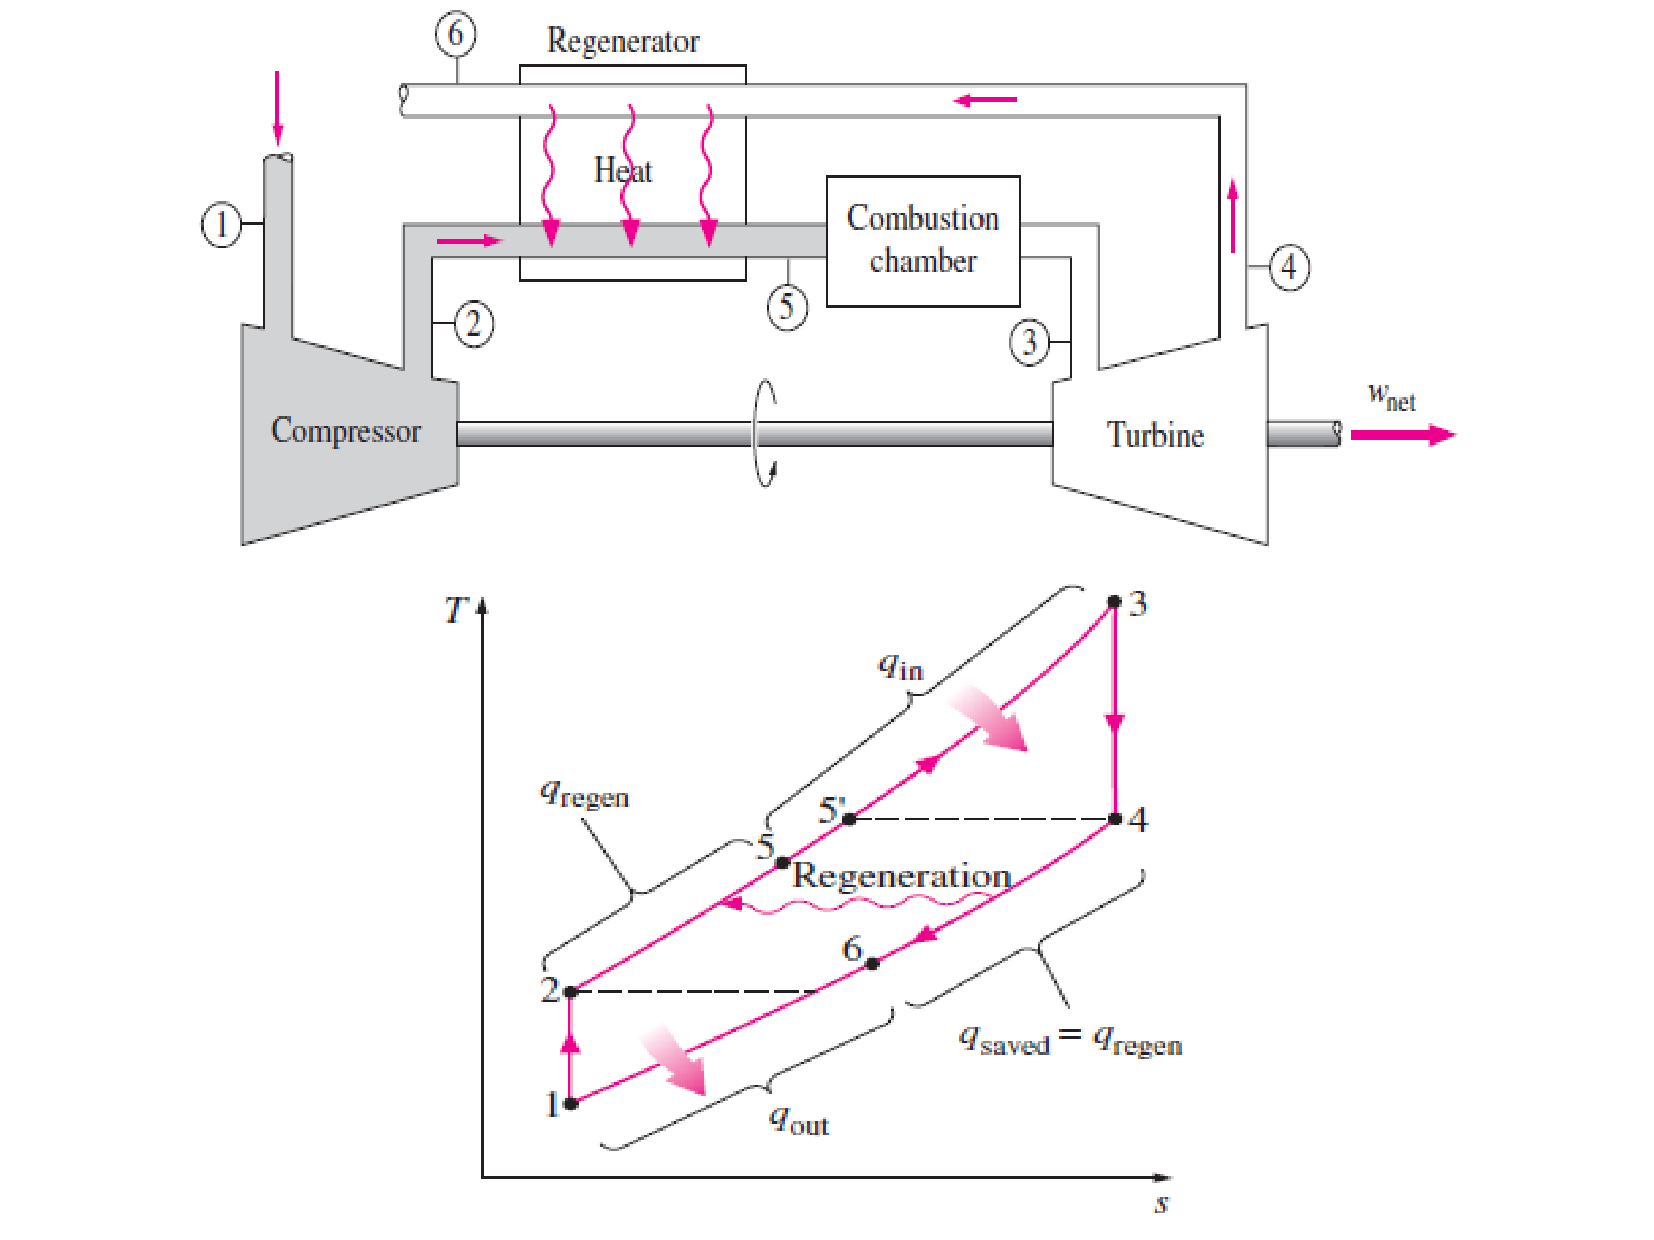
\includegraphics[height=5.cm,width=4.5cm,clip]{./Pics/Brayton_cycle4}
   \end{figure}  
    \end{center}
  \end{column}  
 \end{columns}
\end{frame}


%%%
%%% SECTION
%%%
\section{Summary}

%%%
%%% Slide
%%%
\begin{frame}
 \frametitle{Summary}
  In this Module we studied:
  \begin{enumerate}
   \item<1-> Vapour-based Power Cycles:
    \begin{enumerate}
     \item<3-> Ideal Carnot cycle;
     \item<3-> Rankine and Modified Rankine cycles;
     \item<3-> Components of the cycles (turbine, compressors, heat exchangers etc);
     \item<3-> Thermal analysis of the cycles based on First and Second Laws;
    \end{enumerate}

   \item<2-> Gas-based Power Cycles:
    \begin{enumerate}
     \item<4-> Internal Combustion:
      \begin{enumerate}
       \item<6-> Reciprocating engines;
       \item<6-> Ideal Carnot cycles;
       \item<6-> Otto and Diesel engines;
      \end{enumerate}
     \item<5-> External Combustion:
        \begin{enumerate}
         \item<7-> Brayton Gas Turbine Cycles;
         \item<7-> Thermal and sensitivity analysis of the cycles based on First and Second Laws.
        \end{enumerate}
    \end{enumerate}      

  \end{enumerate}
\end{frame} 



\end{document}
 

%      \vbox{
%         \hbox{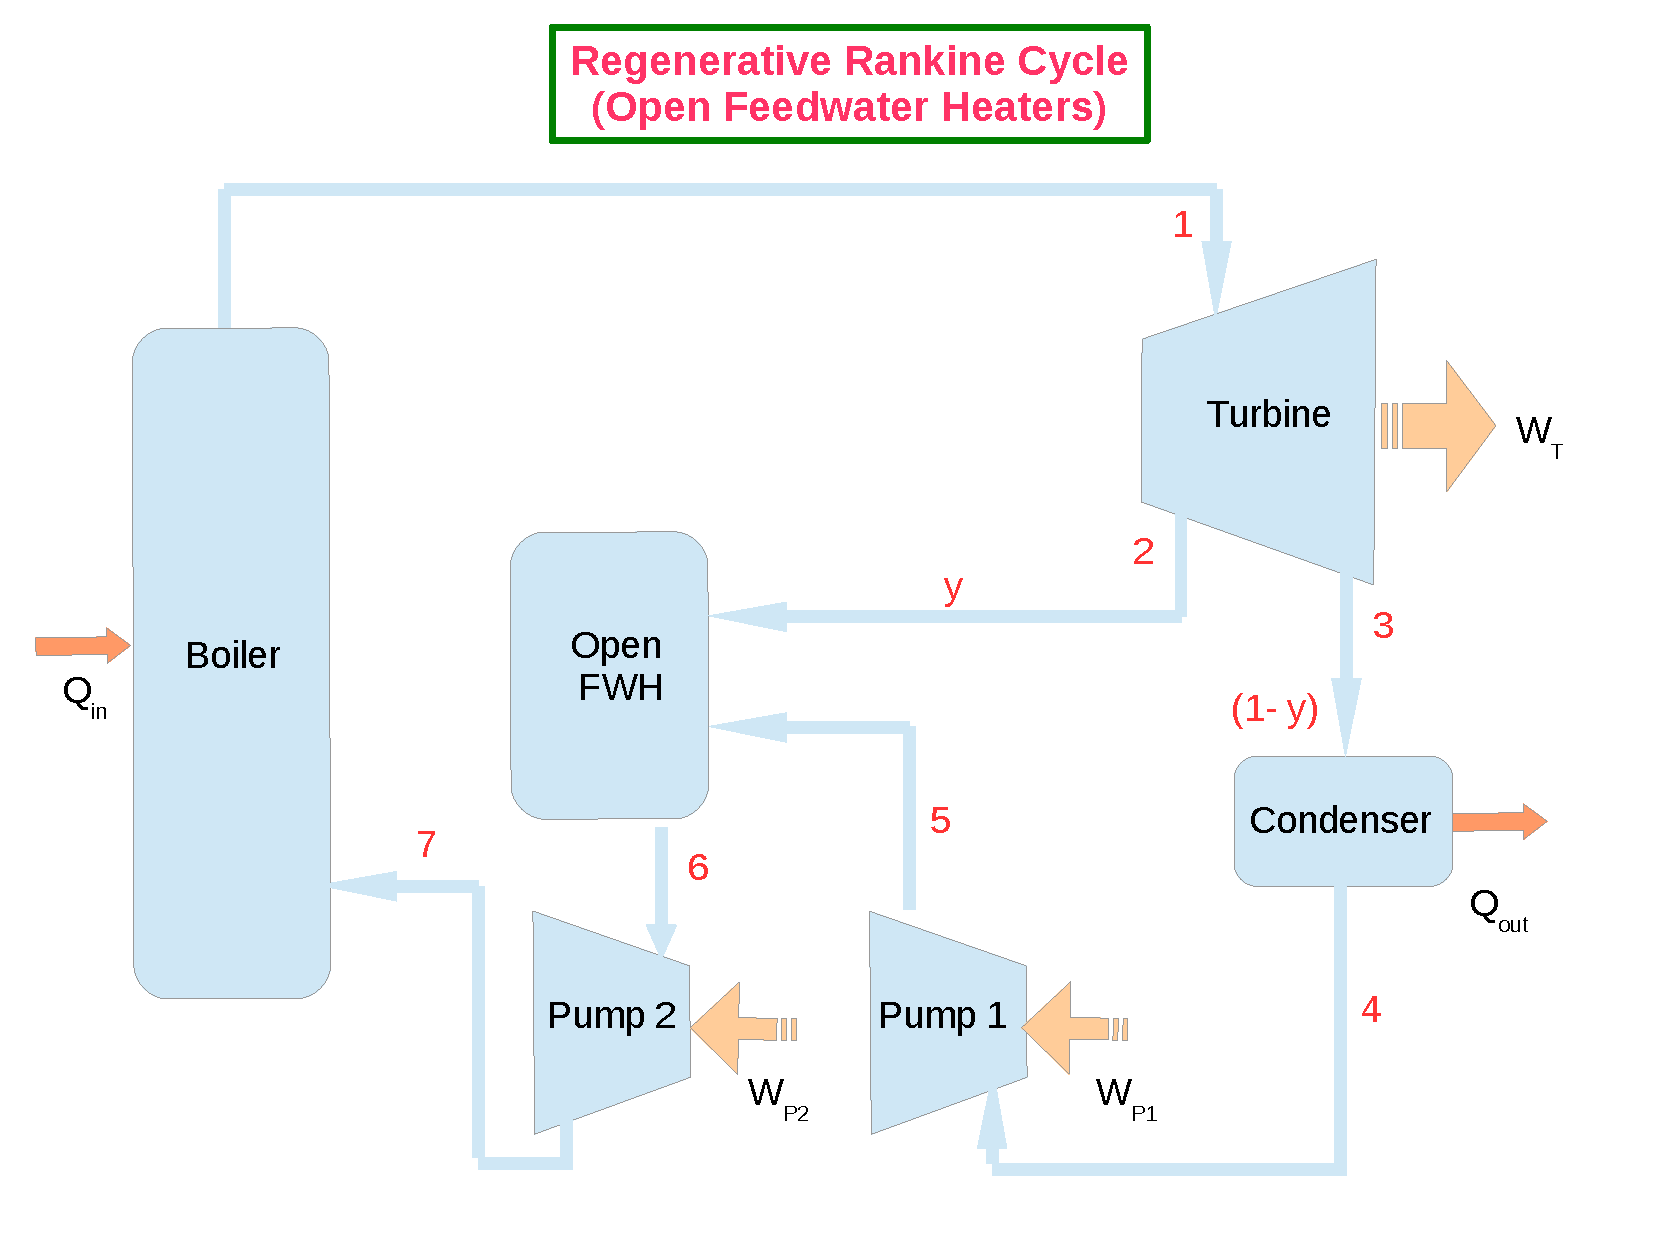
\includegraphics[width=6.cm,clip]{./Pics/RegenerativeOpen_RankineCycle}}
%         \vspace{-0.7cm}
%         \hbox{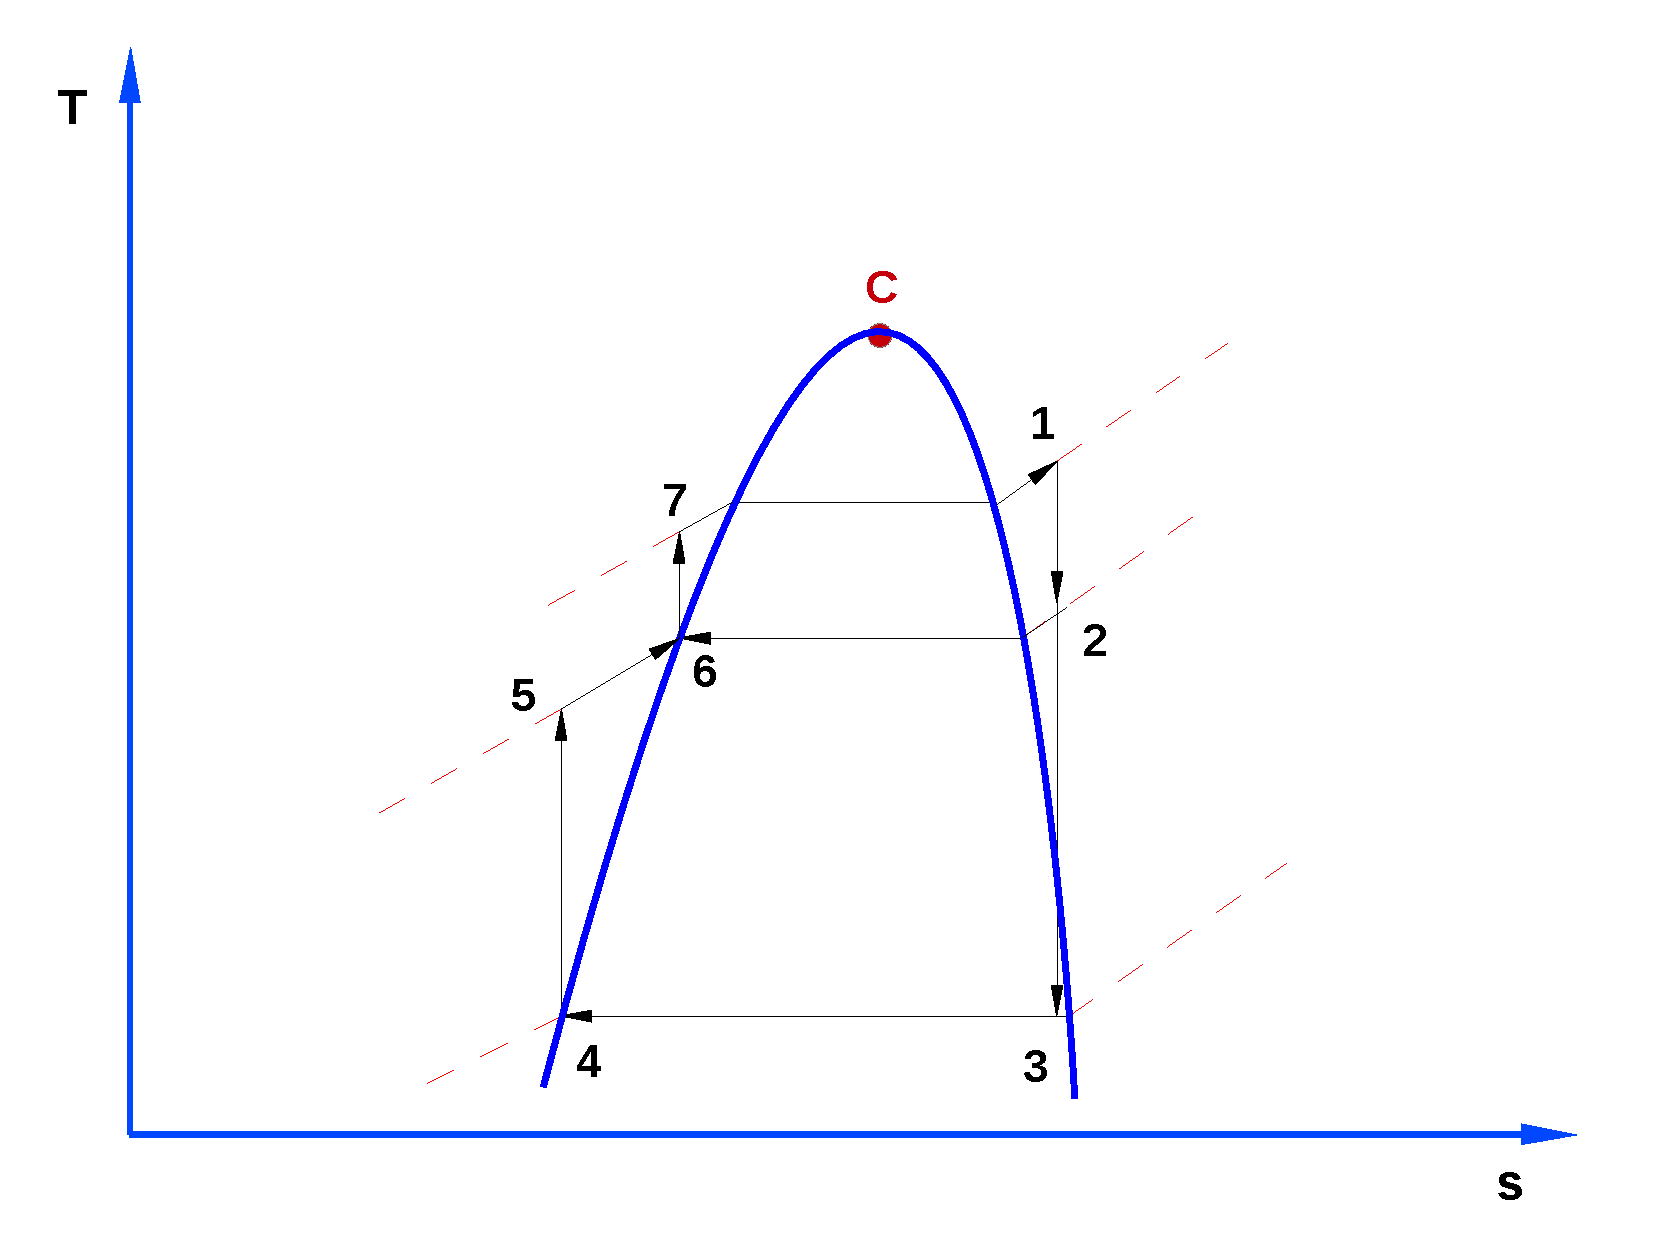
\includegraphics[width=6.cm,clip]{./Pics/RegenerativeOpen_RankineCycle_Diagram}}
%      }  
